\documentclass[
  man,
  longtable,
  nolmodern,
  notxfonts,
  notimes,
  draftfirst,
  colorlinks=true,linkcolor=blue,citecolor=blue,urlcolor=blue]{apa7}

\usepackage{amsmath}
\usepackage{amssymb}




\RequirePackage{longtable}
\RequirePackage{threeparttablex}

\makeatletter
\renewcommand{\paragraph}{\@startsection{paragraph}{4}{\parindent}%
	{0\baselineskip \@plus 0.2ex \@minus 0.2ex}%
	{-.5em}%
	{\normalfont\normalsize\bfseries\typesectitle}}

\renewcommand{\subparagraph}[1]{\@startsection{subparagraph}{5}{0.5em}%
	{0\baselineskip \@plus 0.2ex \@minus 0.2ex}%
	{-\z@\relax}%
	{\normalfont\normalsize\bfseries\itshape\hspace{\parindent}{#1}\textit{\addperi}}{\relax}}
\makeatother




\usepackage{longtable, booktabs, multirow, multicol, colortbl, hhline, caption, array, float, xpatch}
\setcounter{topnumber}{2}
\setcounter{bottomnumber}{2}
\setcounter{totalnumber}{4}
\renewcommand{\topfraction}{0.85}
\renewcommand{\bottomfraction}{0.85}
\renewcommand{\textfraction}{0.15}
\renewcommand{\floatpagefraction}{0.7}

\usepackage{tcolorbox}
\tcbuselibrary{listings,theorems, breakable, skins}
\usepackage{fontawesome5}

\definecolor{quarto-callout-color}{HTML}{909090}
\definecolor{quarto-callout-note-color}{HTML}{0758E5}
\definecolor{quarto-callout-important-color}{HTML}{CC1914}
\definecolor{quarto-callout-warning-color}{HTML}{EB9113}
\definecolor{quarto-callout-tip-color}{HTML}{00A047}
\definecolor{quarto-callout-caution-color}{HTML}{FC5300}
\definecolor{quarto-callout-color-frame}{HTML}{ACACAC}
\definecolor{quarto-callout-note-color-frame}{HTML}{4582EC}
\definecolor{quarto-callout-important-color-frame}{HTML}{D9534F}
\definecolor{quarto-callout-warning-color-frame}{HTML}{F0AD4E}
\definecolor{quarto-callout-tip-color-frame}{HTML}{02B875}
\definecolor{quarto-callout-caution-color-frame}{HTML}{FD7E14}

%\newlength\Oldarrayrulewidth
%\newlength\Oldtabcolsep


\usepackage{hyperref}




\providecommand{\tightlist}{%
  \setlength{\itemsep}{0pt}\setlength{\parskip}{0pt}}
\usepackage{longtable,booktabs,array}
\usepackage{calc} % for calculating minipage widths
% Correct order of tables after \paragraph or \subparagraph
\usepackage{etoolbox}
\makeatletter
\patchcmd\longtable{\par}{\if@noskipsec\mbox{}\fi\par}{}{}
\makeatother
% Allow footnotes in longtable head/foot
\IfFileExists{footnotehyper.sty}{\usepackage{footnotehyper}}{\usepackage{footnote}}
\makesavenoteenv{longtable}

\usepackage{graphicx}
\makeatletter
\newsavebox\pandoc@box
\newcommand*\pandocbounded[1]{% scales image to fit in text height/width
  \sbox\pandoc@box{#1}%
  \Gscale@div\@tempa{\textheight}{\dimexpr\ht\pandoc@box+\dp\pandoc@box\relax}%
  \Gscale@div\@tempb{\linewidth}{\wd\pandoc@box}%
  \ifdim\@tempb\p@<\@tempa\p@\let\@tempa\@tempb\fi% select the smaller of both
  \ifdim\@tempa\p@<\p@\scalebox{\@tempa}{\usebox\pandoc@box}%
  \else\usebox{\pandoc@box}%
  \fi%
}
% Set default figure placement to htbp
\def\fps@figure{htbp}
\makeatother


% definitions for citeproc citations
\NewDocumentCommand\citeproctext{}{}
\NewDocumentCommand\citeproc{mm}{%
  \begingroup\def\citeproctext{#2}\cite{#1}\endgroup}
\makeatletter
 % allow citations to break across lines
 \let\@cite@ofmt\@firstofone
 % avoid brackets around text for \cite:
 \def\@biblabel#1{}
 \def\@cite#1#2{{#1\if@tempswa , #2\fi}}
\makeatother
\newlength{\cslhangindent}
\setlength{\cslhangindent}{1.5em}
\newlength{\csllabelwidth}
\setlength{\csllabelwidth}{3em}
\newenvironment{CSLReferences}[2] % #1 hanging-indent, #2 entry-spacing
 {\begin{list}{}{%
  \setlength{\itemindent}{0pt}
  \setlength{\leftmargin}{0pt}
  \setlength{\parsep}{0pt}
  % turn on hanging indent if param 1 is 1
  \ifodd #1
   \setlength{\leftmargin}{\cslhangindent}
   \setlength{\itemindent}{-1\cslhangindent}
  \fi
  % set entry spacing
  \setlength{\itemsep}{#2\baselineskip}}}
 {\end{list}}
\usepackage{calc}
\newcommand{\CSLBlock}[1]{\hfill\break\parbox[t]{\linewidth}{\strut\ignorespaces#1\strut}}
\newcommand{\CSLLeftMargin}[1]{\parbox[t]{\csllabelwidth}{\strut#1\strut}}
\newcommand{\CSLRightInline}[1]{\parbox[t]{\linewidth - \csllabelwidth}{\strut#1\strut}}
\newcommand{\CSLIndent}[1]{\hspace{\cslhangindent}#1}





\usepackage{newtx}

\defaultfontfeatures{Scale=MatchLowercase}
\defaultfontfeatures[\rmfamily]{Ligatures=TeX,Scale=1}





\title{EEG-ECMR}


\shorttitle{EEG-ECMR}


\usepackage{etoolbox}






\author{Jordan B Gunn}



\affiliation{
{Department of Psychology, University of Cambridge}}




\leftheader{Gunn}

\date{2026-03-15}





\authornote{ 

\par{       }
}

\makeatletter
\let\endoldlt\endlongtable
\def\endlongtable{
\hline
\endoldlt
}
\makeatother
\RequirePackage{longtable}
\DeclareDelayedFloatFlavor{longtable}{table}

\urlstyle{same}



\makeatletter
\@ifpackageloaded{caption}{}{\usepackage{caption}}
\AtBeginDocument{%
\ifdefined\contentsname
  \renewcommand*\contentsname{Table of contents}
\else
  \newcommand\contentsname{Table of contents}
\fi
\ifdefined\listfigurename
  \renewcommand*\listfigurename{List of Figures}
\else
  \newcommand\listfigurename{List of Figures}
\fi
\ifdefined\listtablename
  \renewcommand*\listtablename{List of Tables}
\else
  \newcommand\listtablename{List of Tables}
\fi
\ifdefined\figurename
  \renewcommand*\figurename{Figure}
\else
  \newcommand\figurename{Figure}
\fi
\ifdefined\tablename
  \renewcommand*\tablename{Table}
\else
  \newcommand\tablename{Table}
\fi
}
\@ifpackageloaded{float}{}{\usepackage{float}}
\floatstyle{ruled}
\@ifundefined{c@chapter}{\newfloat{codelisting}{h}{lop}}{\newfloat{codelisting}{h}{lop}[chapter]}
\floatname{codelisting}{Listing}
\newcommand*\listoflistings{\listof{codelisting}{List of Listings}}
\makeatother
\makeatletter
\makeatother
\makeatletter
\@ifpackageloaded{caption}{}{\usepackage{caption}}
\@ifpackageloaded{subcaption}{}{\usepackage{subcaption}}
\makeatother

% From https://tex.stackexchange.com/a/645996/211326
%%% apa7 doesn't want to add appendix section titles in the toc
%%% let's make it do it
\makeatletter
\xpatchcmd{\appendix}
  {\par}
  {\addcontentsline{toc}{section}{\@currentlabelname}\par}
  {}{}
\makeatother

%% Disable longtable counter
%% https://tex.stackexchange.com/a/248395/211326

\usepackage{etoolbox}

\makeatletter
\patchcmd{\LT@caption}
  {\bgroup}
  {\bgroup\global\LTpatch@captiontrue}
  {}{}
\patchcmd{\longtable}
  {\par}
  {\par\global\LTpatch@captionfalse}
  {}{}
\apptocmd{\endlongtable}
  {\ifLTpatch@caption\else\addtocounter{table}{-1}\fi}
  {}{}
\newif\ifLTpatch@caption
\makeatother

\begin{document}

\maketitle


\setcounter{secnumdepth}{5}

\setlength\LTleft{0pt}


This document records our progress and key decisions as we build a
brain-based version of eCMR using EEG data from Zarubin et al.~(2020).

Prior analyses provide two anchors. First, emotionally negative items
are recalled more often than neutral items. Second, late positive
potential (LPP) amplitudes during study predict later recall for
emotional items but not neutral items. These patterns relate brain
signals and emotion to performance but do not specify mechanisms that
generate recall.

We address this with computational neurocognitive models that formalize
hypotheses about how LPPs interact with attention and context binding at
encoding. We simulate trials and score models by the likelihood they
assign to the full recalled set on each list, asking how probable the
observed data are under each mechanism as specified. Good fits provide
evidence that a mechanism can produce the behavior; poor fits indicate
that the specification is insufficient.

Our evaluation instantiates these hypotheses within the
retrieved-context framework of eCMR (Talmi et al., 2019), where
item--context associations guide recall. Emotional items receive a
learning boost and LPP modulates that boost, increasing their odds of
retrieval. We compare ways LPPs could modulate these processes and
assess which specification renders the observed recalled sets most
probable, moving beyond correlation toward mechanism.

\section{Data Preparation}\label{data-preparation}

Lists are analyzed as 20‑item sequences because the first two study
positions were removed during preprocessing by Zarubin et al to avoid
primacy confounds and cannot be recovered. As a result, each trial
contributes only the remaining 20 items to all analyses and modeling.

The primary analysis table is
\texttt{Single\_Trial\_Behavioural\_and\_EEG\_Data\_Z.csv}
(\texttt{Z:\textbackslash{}Talmi\ lab\ space\textbackslash{}Archive\textbackslash{}Secondary\_Data\_Analysis\_Zarubin\_From\_Robin\textbackslash{}Manuscript\textbackslash{}files\ from\ robin\ nov24\textbackslash{}}).
It omits study events that lack reliable EEG measurements, so we merged
it with the behavioral log \texttt{All\_Included\_Subjects.csv}
(\texttt{Z:\textbackslash{}Talmi\ lab\ space\textbackslash{}Archive\textbackslash{}Secondary\_Data\_Analysis\_Zarubin\_From\_Robin\textbackslash{}Data\textbackslash{}Behaviour\textbackslash{}Behaviour\_csv\_files\textbackslash{}})
to restore recall status for those events. Before merging, we verified
label consistency across sources and found no conflicts between recalled
vs not‑recalled designations.

The merged dataset comprises 6,840 study events from 342 list trials
with 20 analyzable items per list. Overall missingness is
\textasciitilde5\% and balanced across valence: 371 events (5.42\%) lack
EEG measurements, with negative lists contributing 125 of 2,266 events
(5.52\%; mean 0.37 ± 0.65 items missing per trial) and neutral lists
contributing 246 of 4,574 events (5.38\%; mean 0.72 ± 0.93 items missing
per trial). In total, 202 of 342 lists (59.1\%) include at least one
missing LPP value; among affected lists, 1.84 ± 1.01 items are missing
(median 2; maximum 6). Across participants, missing exposure ranges from
2 to 19 items (3.9--10\% of each person's 180 study events), so
imputation is methodologically substantive.

LPP amplitudes are imputed using within-person, within-trial
emotion‑matched means. For any study event still missing an LPP value
after merging, we fill that participant's average for items of the same
emotion within the same trial. This preserves within‑person,
within‑trial, and emotion‑specific structure and avoids borrowing
information across trials or valence conditions.

The dataset indicates which items were recalled but not their order.
Accordingly, model fitting must use loss functions defined over the
recalled set per trial, and analyses of recall structure require
order‑agnostic alternatives.

\section{Benchmark Analyses}\label{benchmark-analyses}

These benchmarks both define concrete targets for model development and
verify that data preparation preserved known effects. Unless noted,
error bars show 95\% bootstrap confidence intervals across participants,
computed by resampling participants with replacement 10,000 times and
taking the 2.5th and 97.5th percentiles of the resulting distribution as
confidence bounds.

\subsection{Emotional Items Are Recalled More
Often}\label{emotional-items-are-recalled-more-often}

The central behavioral pattern is the emotional enhancement of memory
(EEM): emotionally negative items are recalled more often than neutral
items. We benchmark EEM with a categorized serial position curve
(Category-SPC). For each study position (1-20), we tabulate recall rates
separately for emotional and neutral items. Emotional items are recalled
more often across all study positions, replicating the reference
analysis used in the Daw meeting slides and confirming our data
pipeline. Effect summary: mean recall difference (emotional -- neutral),
averaged across positions = 0.125, 95\%\,CI {[}0.090,\,0.162{]};
positions with emotional \textgreater{} neutral = 20/20.

\begin{figure}

\caption{\label{fig-reference_catspc}Recall rate by study position and
item type from reference materials (LEFT) and from the present dataset
(RIGHT).}

\begin{minipage}{0.50\linewidth}
\pandocbounded{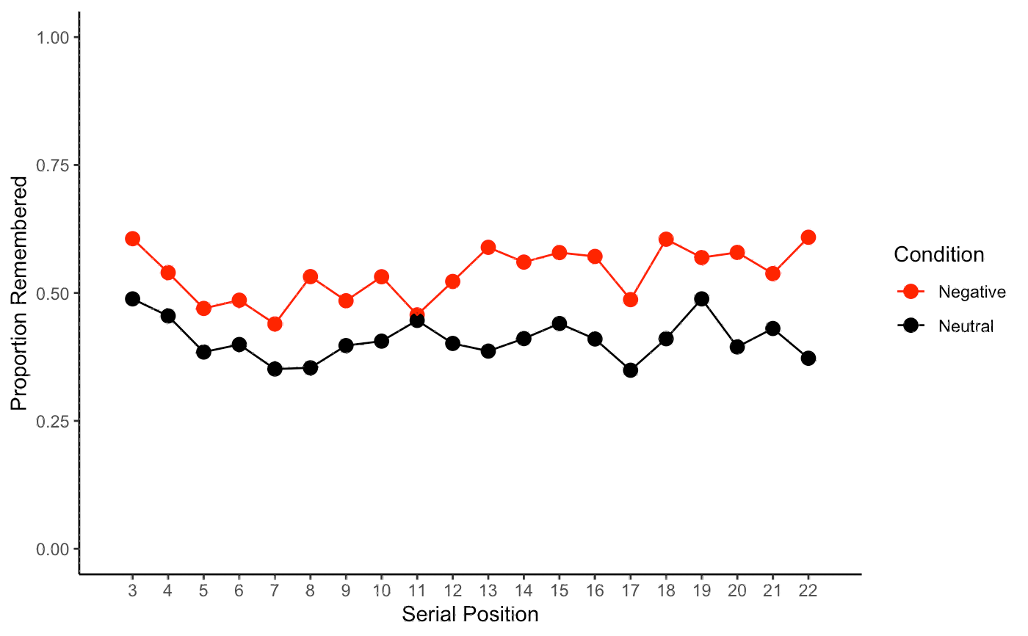
\includegraphics[keepaspectratio]{results/figures/daw_meeting_slide5.png}}\end{minipage}%
%
\begin{minipage}{0.50\linewidth}
\pandocbounded{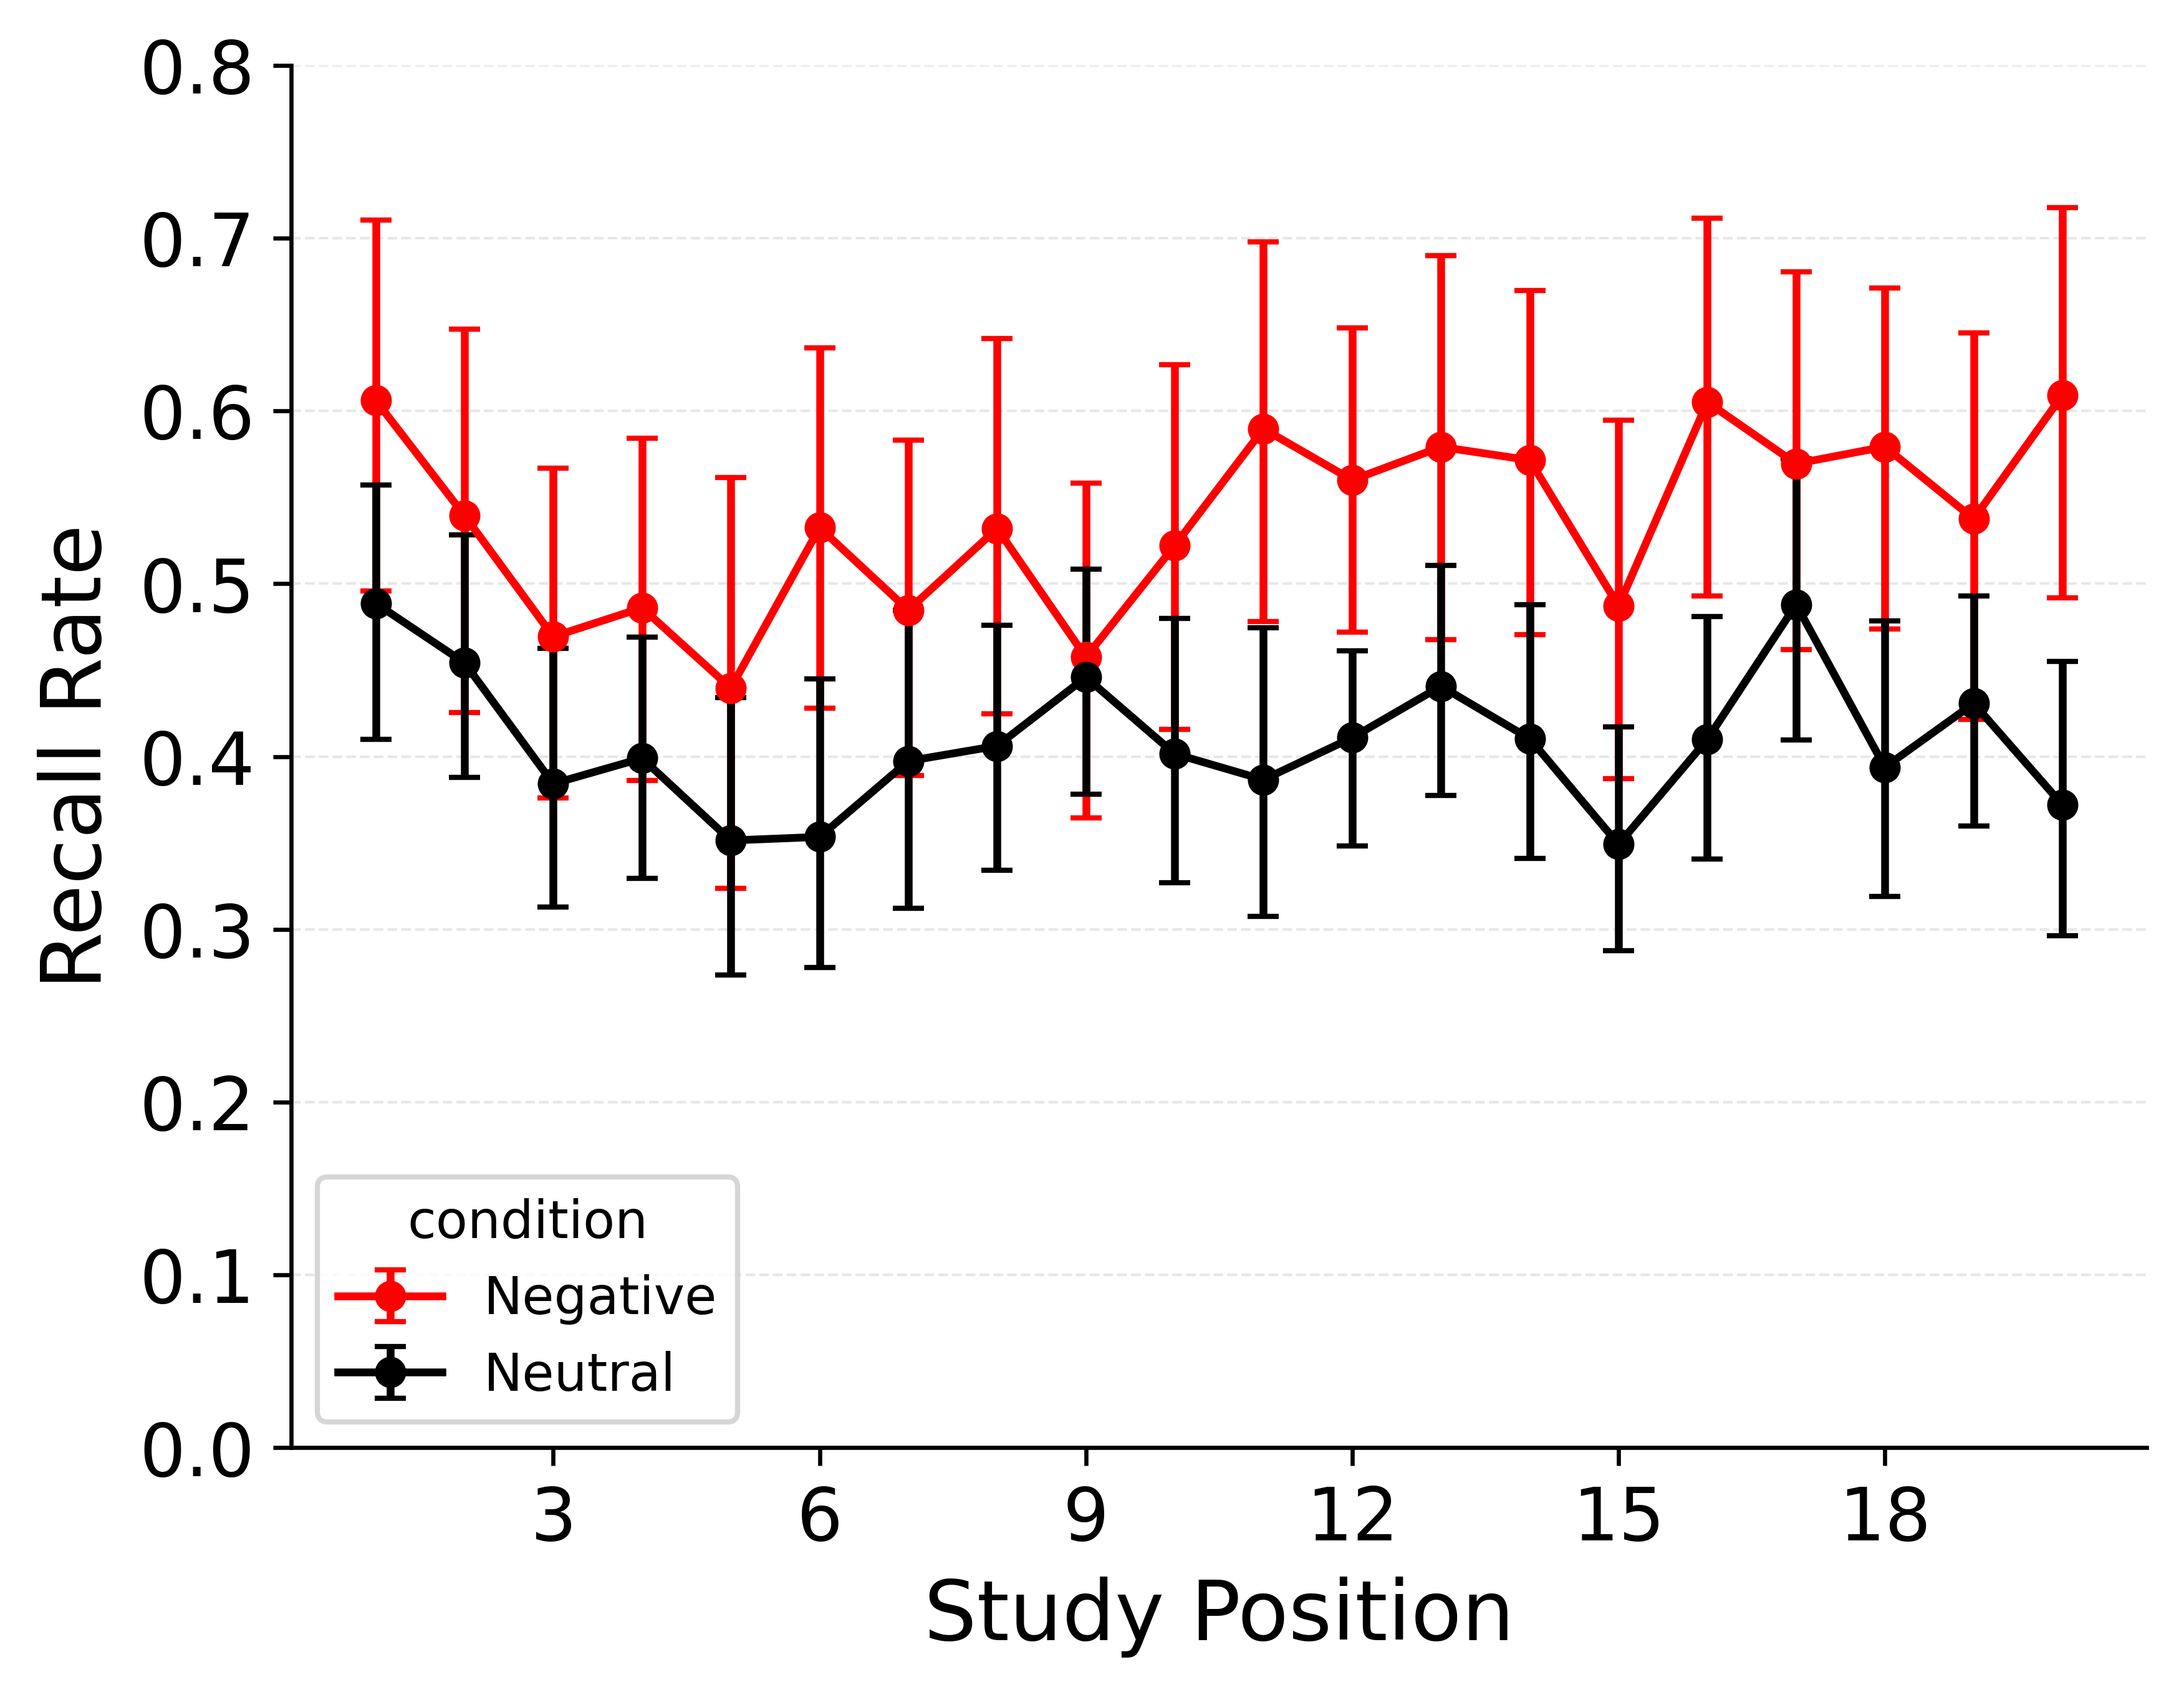
\includegraphics[keepaspectratio]{results/figures/analyses/reference_catspc.png}}\end{minipage}%

\end{figure}%

\subsection{LPP Is Higher for Emotional
Items}\label{lpp-is-higher-for-emotional-items}

We examine LPP amplitudes by study position and item type, separately
for Early LPP (400-700 ms) and Late LPP (700-1,000 ms). In both windows,
mean LPPs are higher for emotional items than for neutral items across
positions, but variability is large and position-wise means fluctuate,
so distributions overlap substantially. This motivates treating LPP and
item type as distinct signals. Effect summary: mean Early-LPP difference
(emotional - neutral) across positions = 0.405 µV, 95\% CI {[}0.280,
0.516{]}; Late-LPP difference = 0.354 µV, 95\% CI {[}0.219, 0.484{]};
standardized difference (Cohen's d\_Early, d\_Late) = 0.23, 0.18.

\begin{figure}

\caption{\label{fig-cat_lpp_spc}LPP by study position and item type.
Early window (LEFT), Late window (RIGHT).}

\begin{minipage}{0.50\linewidth}
\pandocbounded{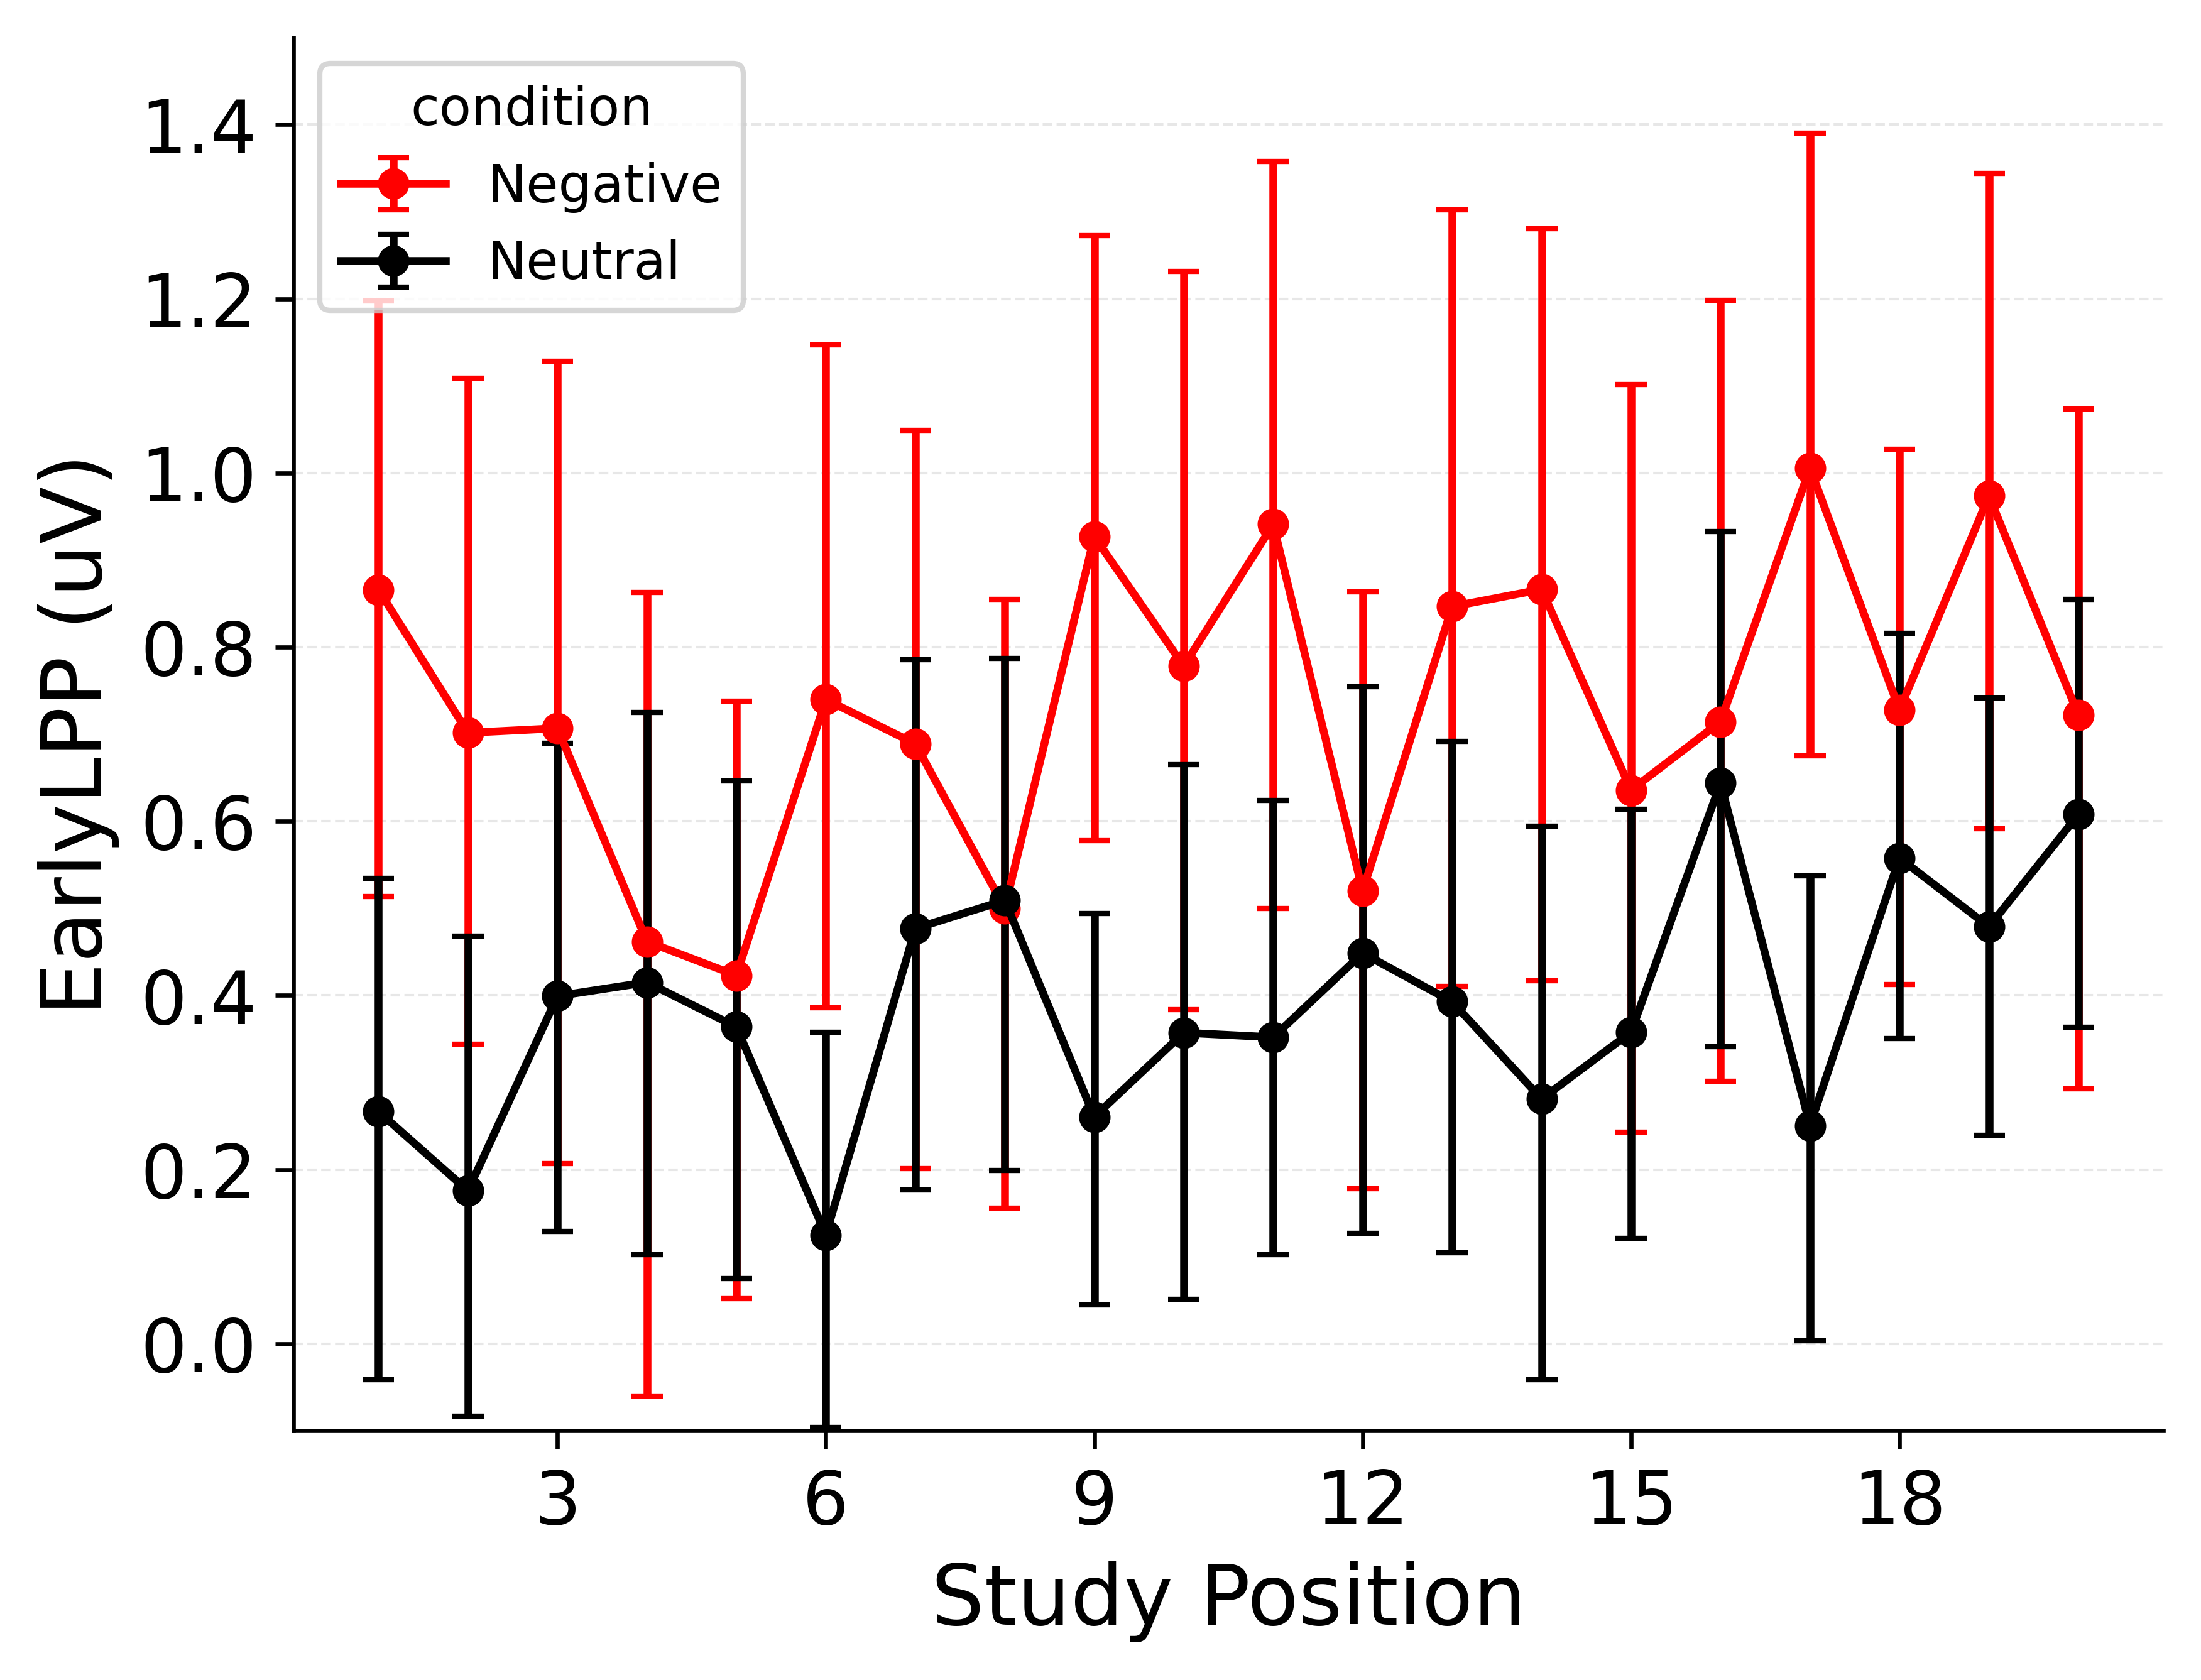
\includegraphics[keepaspectratio]{results/figures/analyses/cat_lpp_spc_EarlyLPP.png}}\end{minipage}%
%
\begin{minipage}{0.50\linewidth}
\pandocbounded{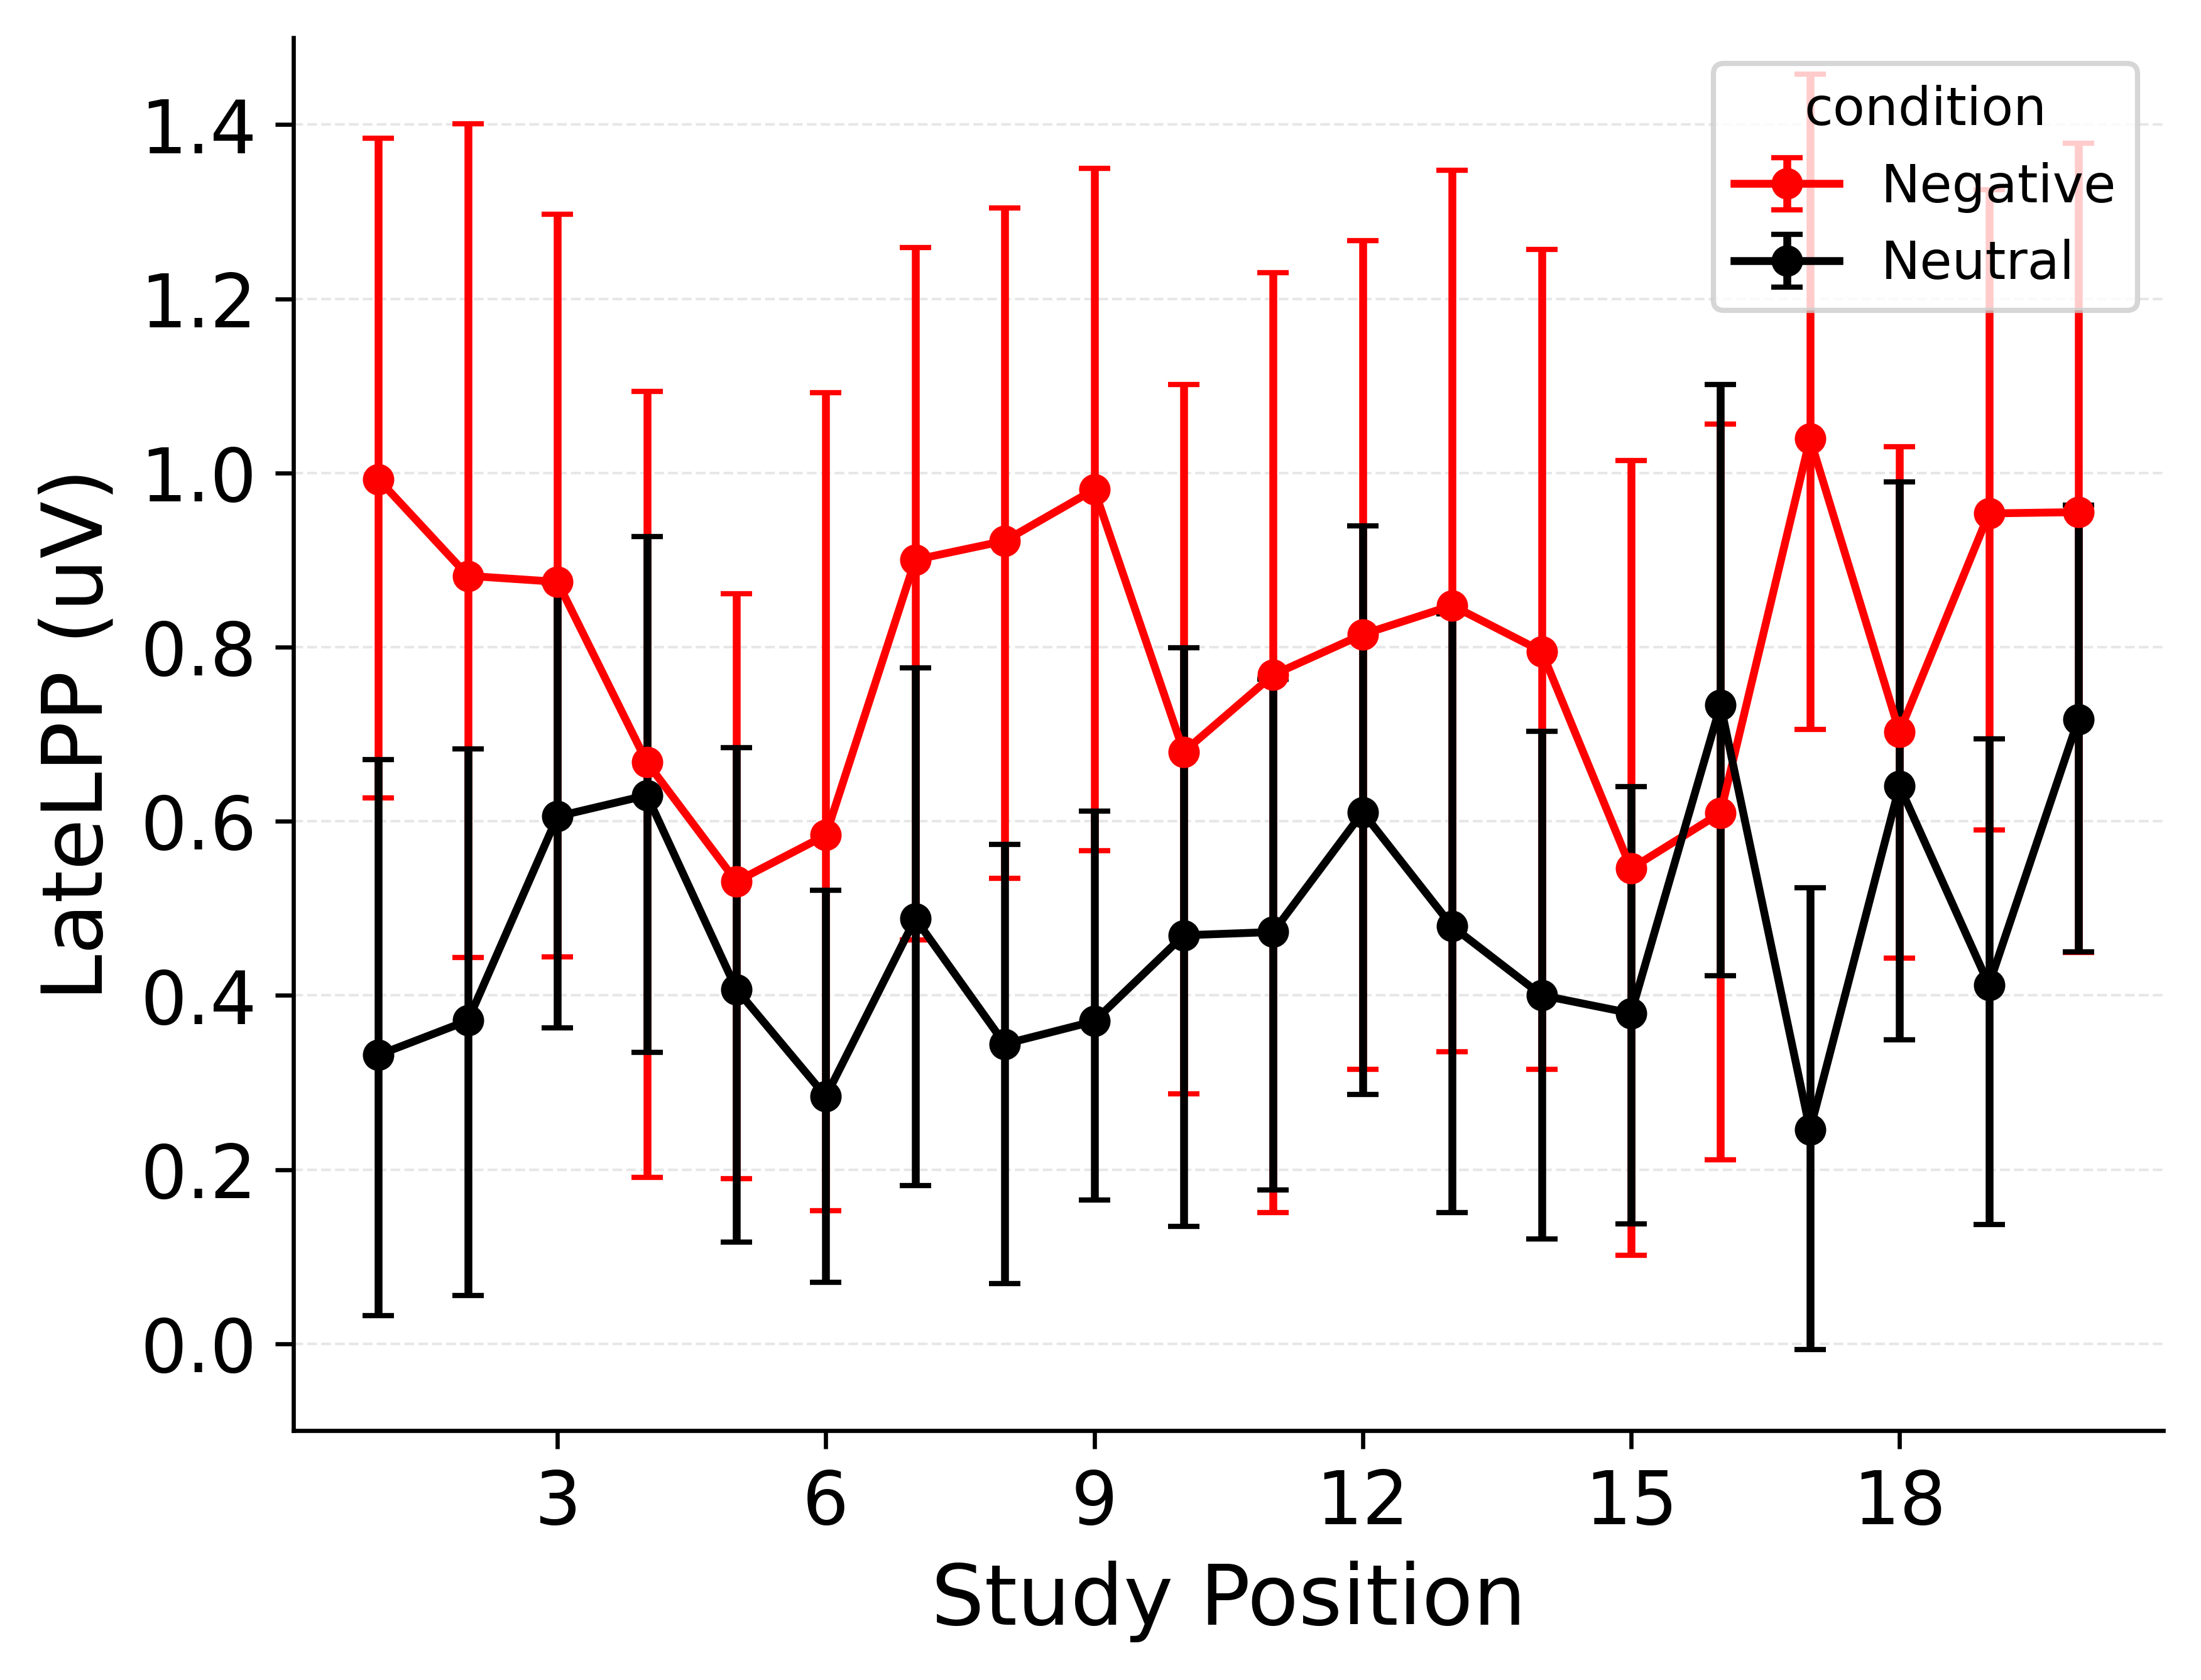
\includegraphics[keepaspectratio]{results/figures/analyses/cat_lpp_spc_LateLPP.png}}\end{minipage}%

\end{figure}%

\subsection{LPP Predicts Recall More Strongly for Emotional
Items}\label{lpp-predicts-recall-more-strongly-for-emotional-items}

To relate LPP to behavior, we plot LPP by study position and recall
status, with separate plots by item type and LPP window
Figure~\ref{fig-cat_lpp_by_recall_split}. The clearest separation is in
the Early window for emotional items: recalled emotional items show
higher Early LPPs than unrecalled emotional items, whereas neutral items
show only a small recalled vs unrecalled difference. Effect summary:
Early-LPP difference (recalled - unrecalled) for emotional items = 0.43
µV, 95\% CI {[}0.27, 0.58{]}; for neutral items the corresponding
estimate is 0.10 µV, 95\% CI {[}-0.07, 0.28{]}. Late-window differences
(emotional, neutral) are smaller: 0.20 µV {[}0.04, 0.38{]} and 0.03 µV
{[}-0.14, 0.20{]}, respectively.

\begin{figure}

\caption{\label{fig-cat_lpp_by_recall_split}LPP by recall status and
item type: Early LPP (TOP row) and Late LPP (BOTTOM row), split by
NEGATIVE items (LEFT) and NEUTRAL items (RIGHT).}

\begin{minipage}{0.50\linewidth}
\pandocbounded{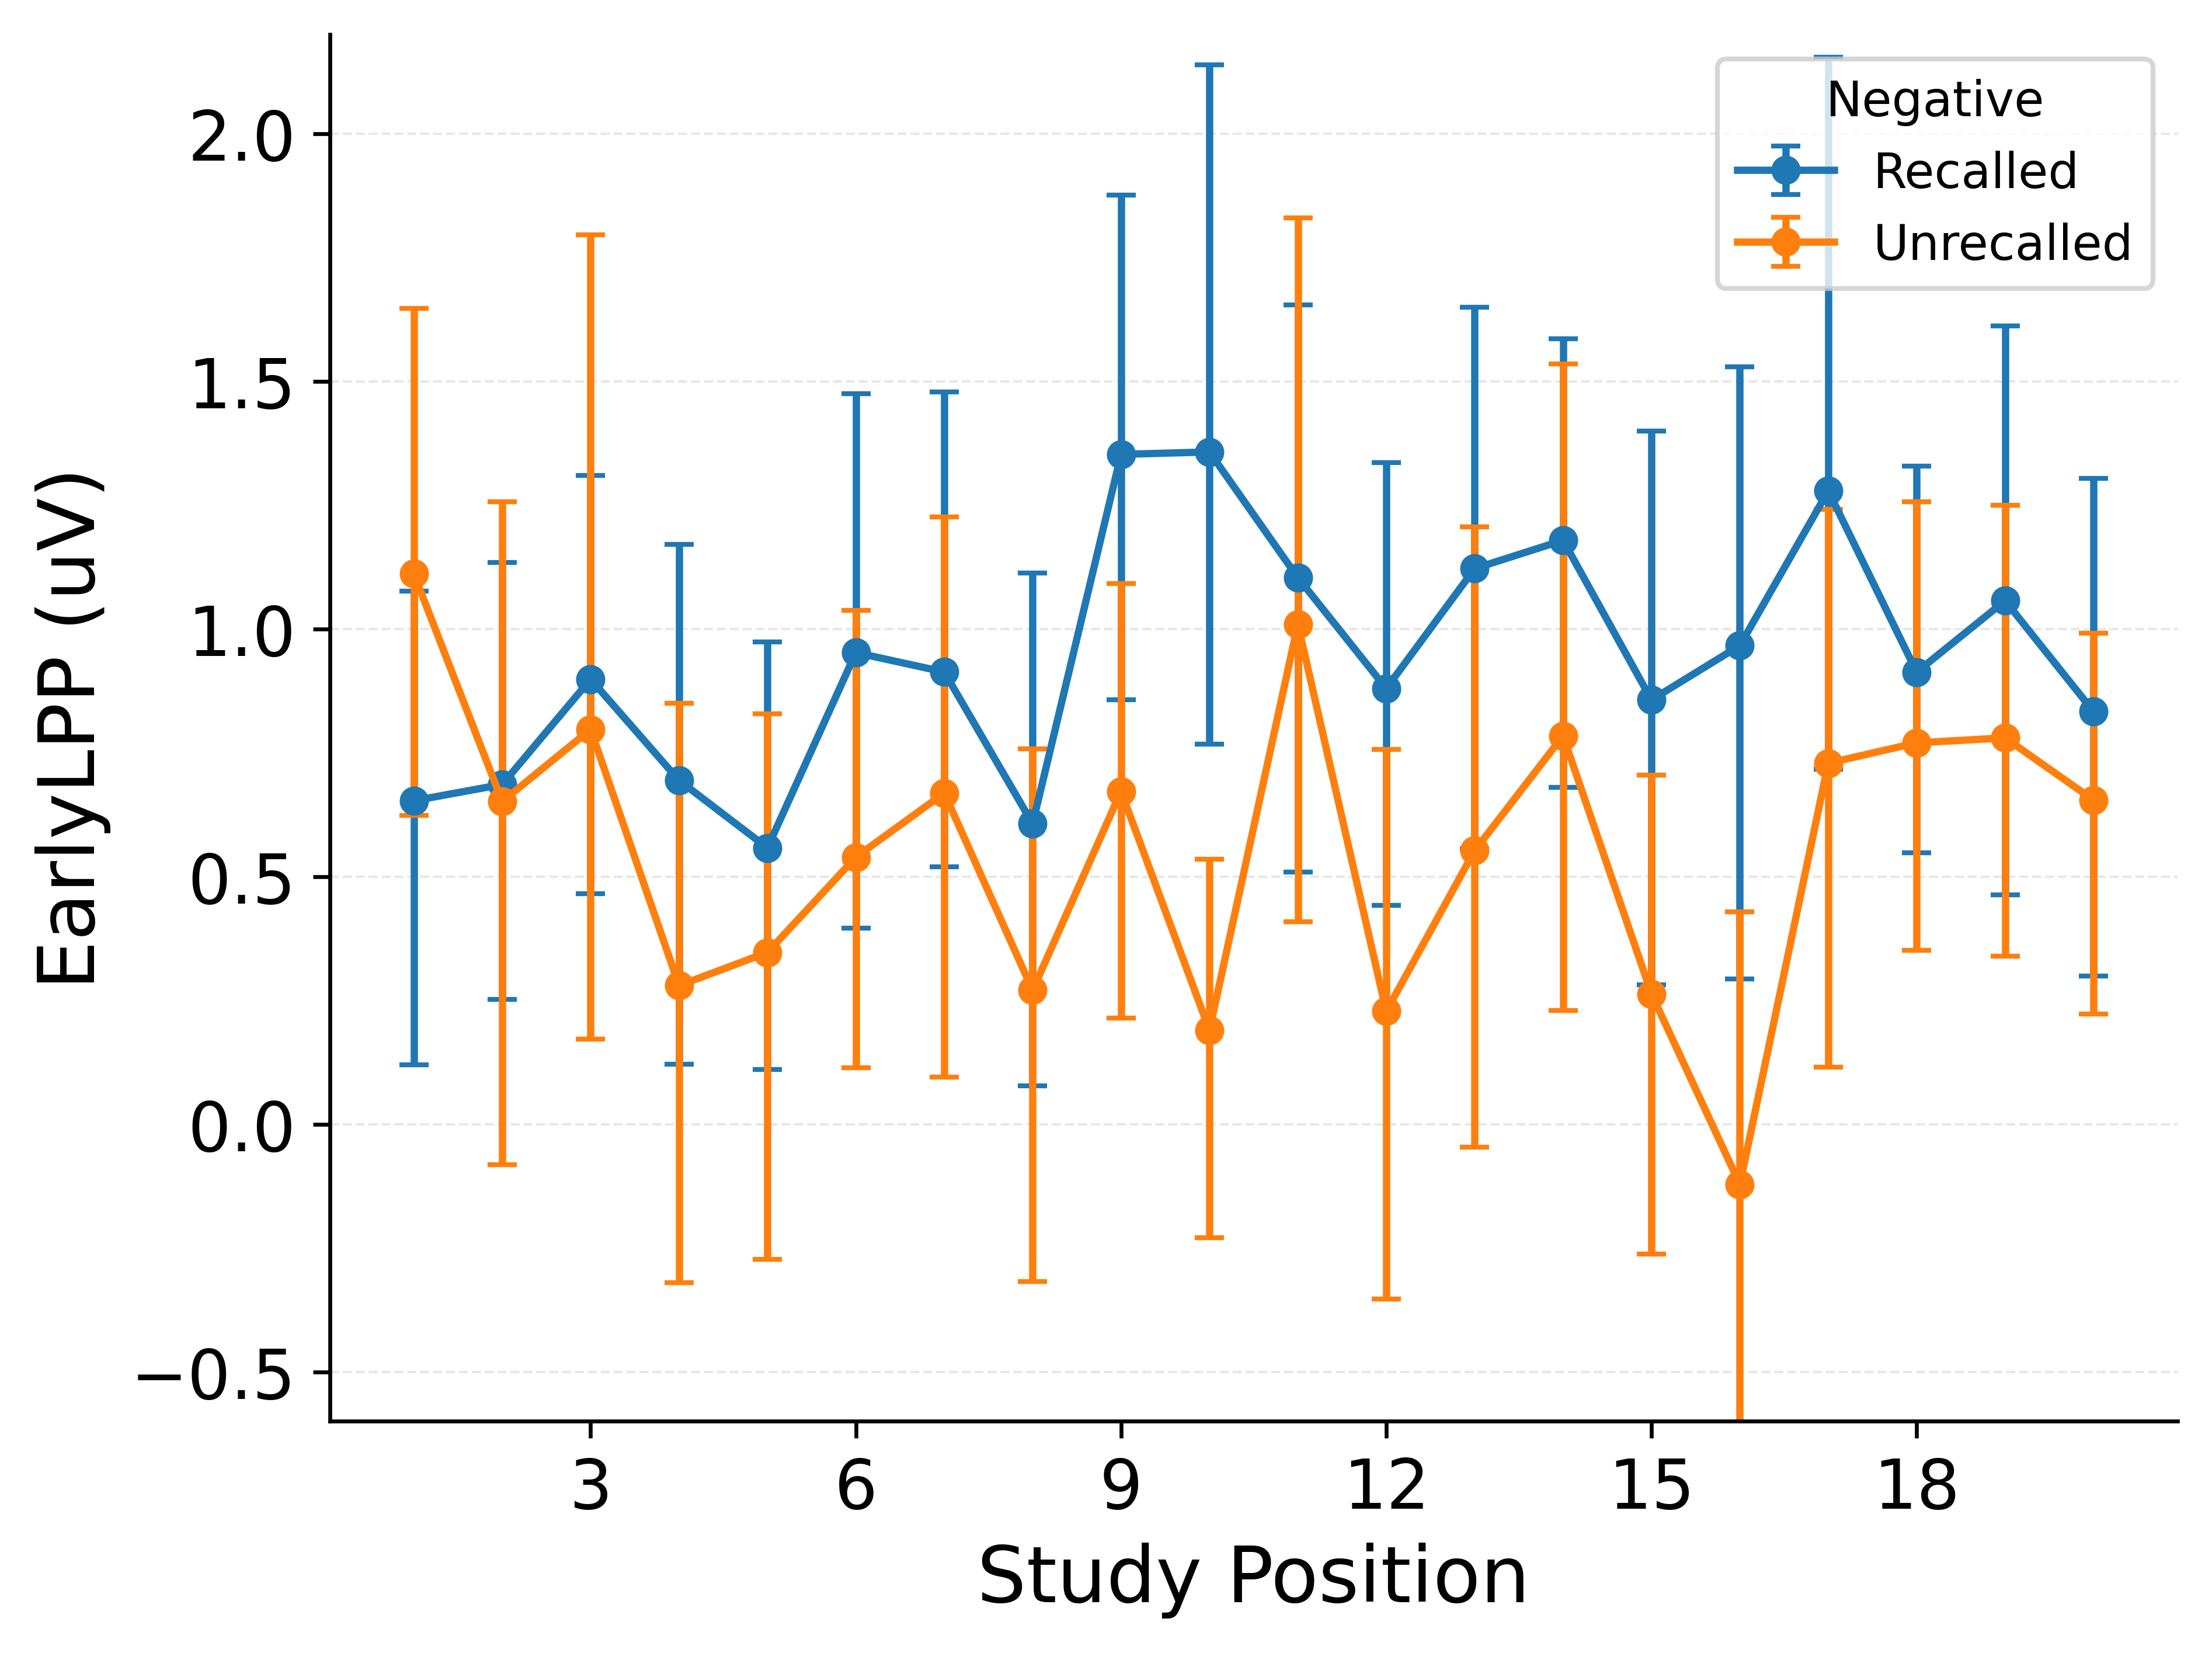
\includegraphics[keepaspectratio]{results/figures/analyses/cat_lpp_by_recall_EarlyLPP_Negative.png}}\end{minipage}%
%
\begin{minipage}{0.50\linewidth}
\pandocbounded{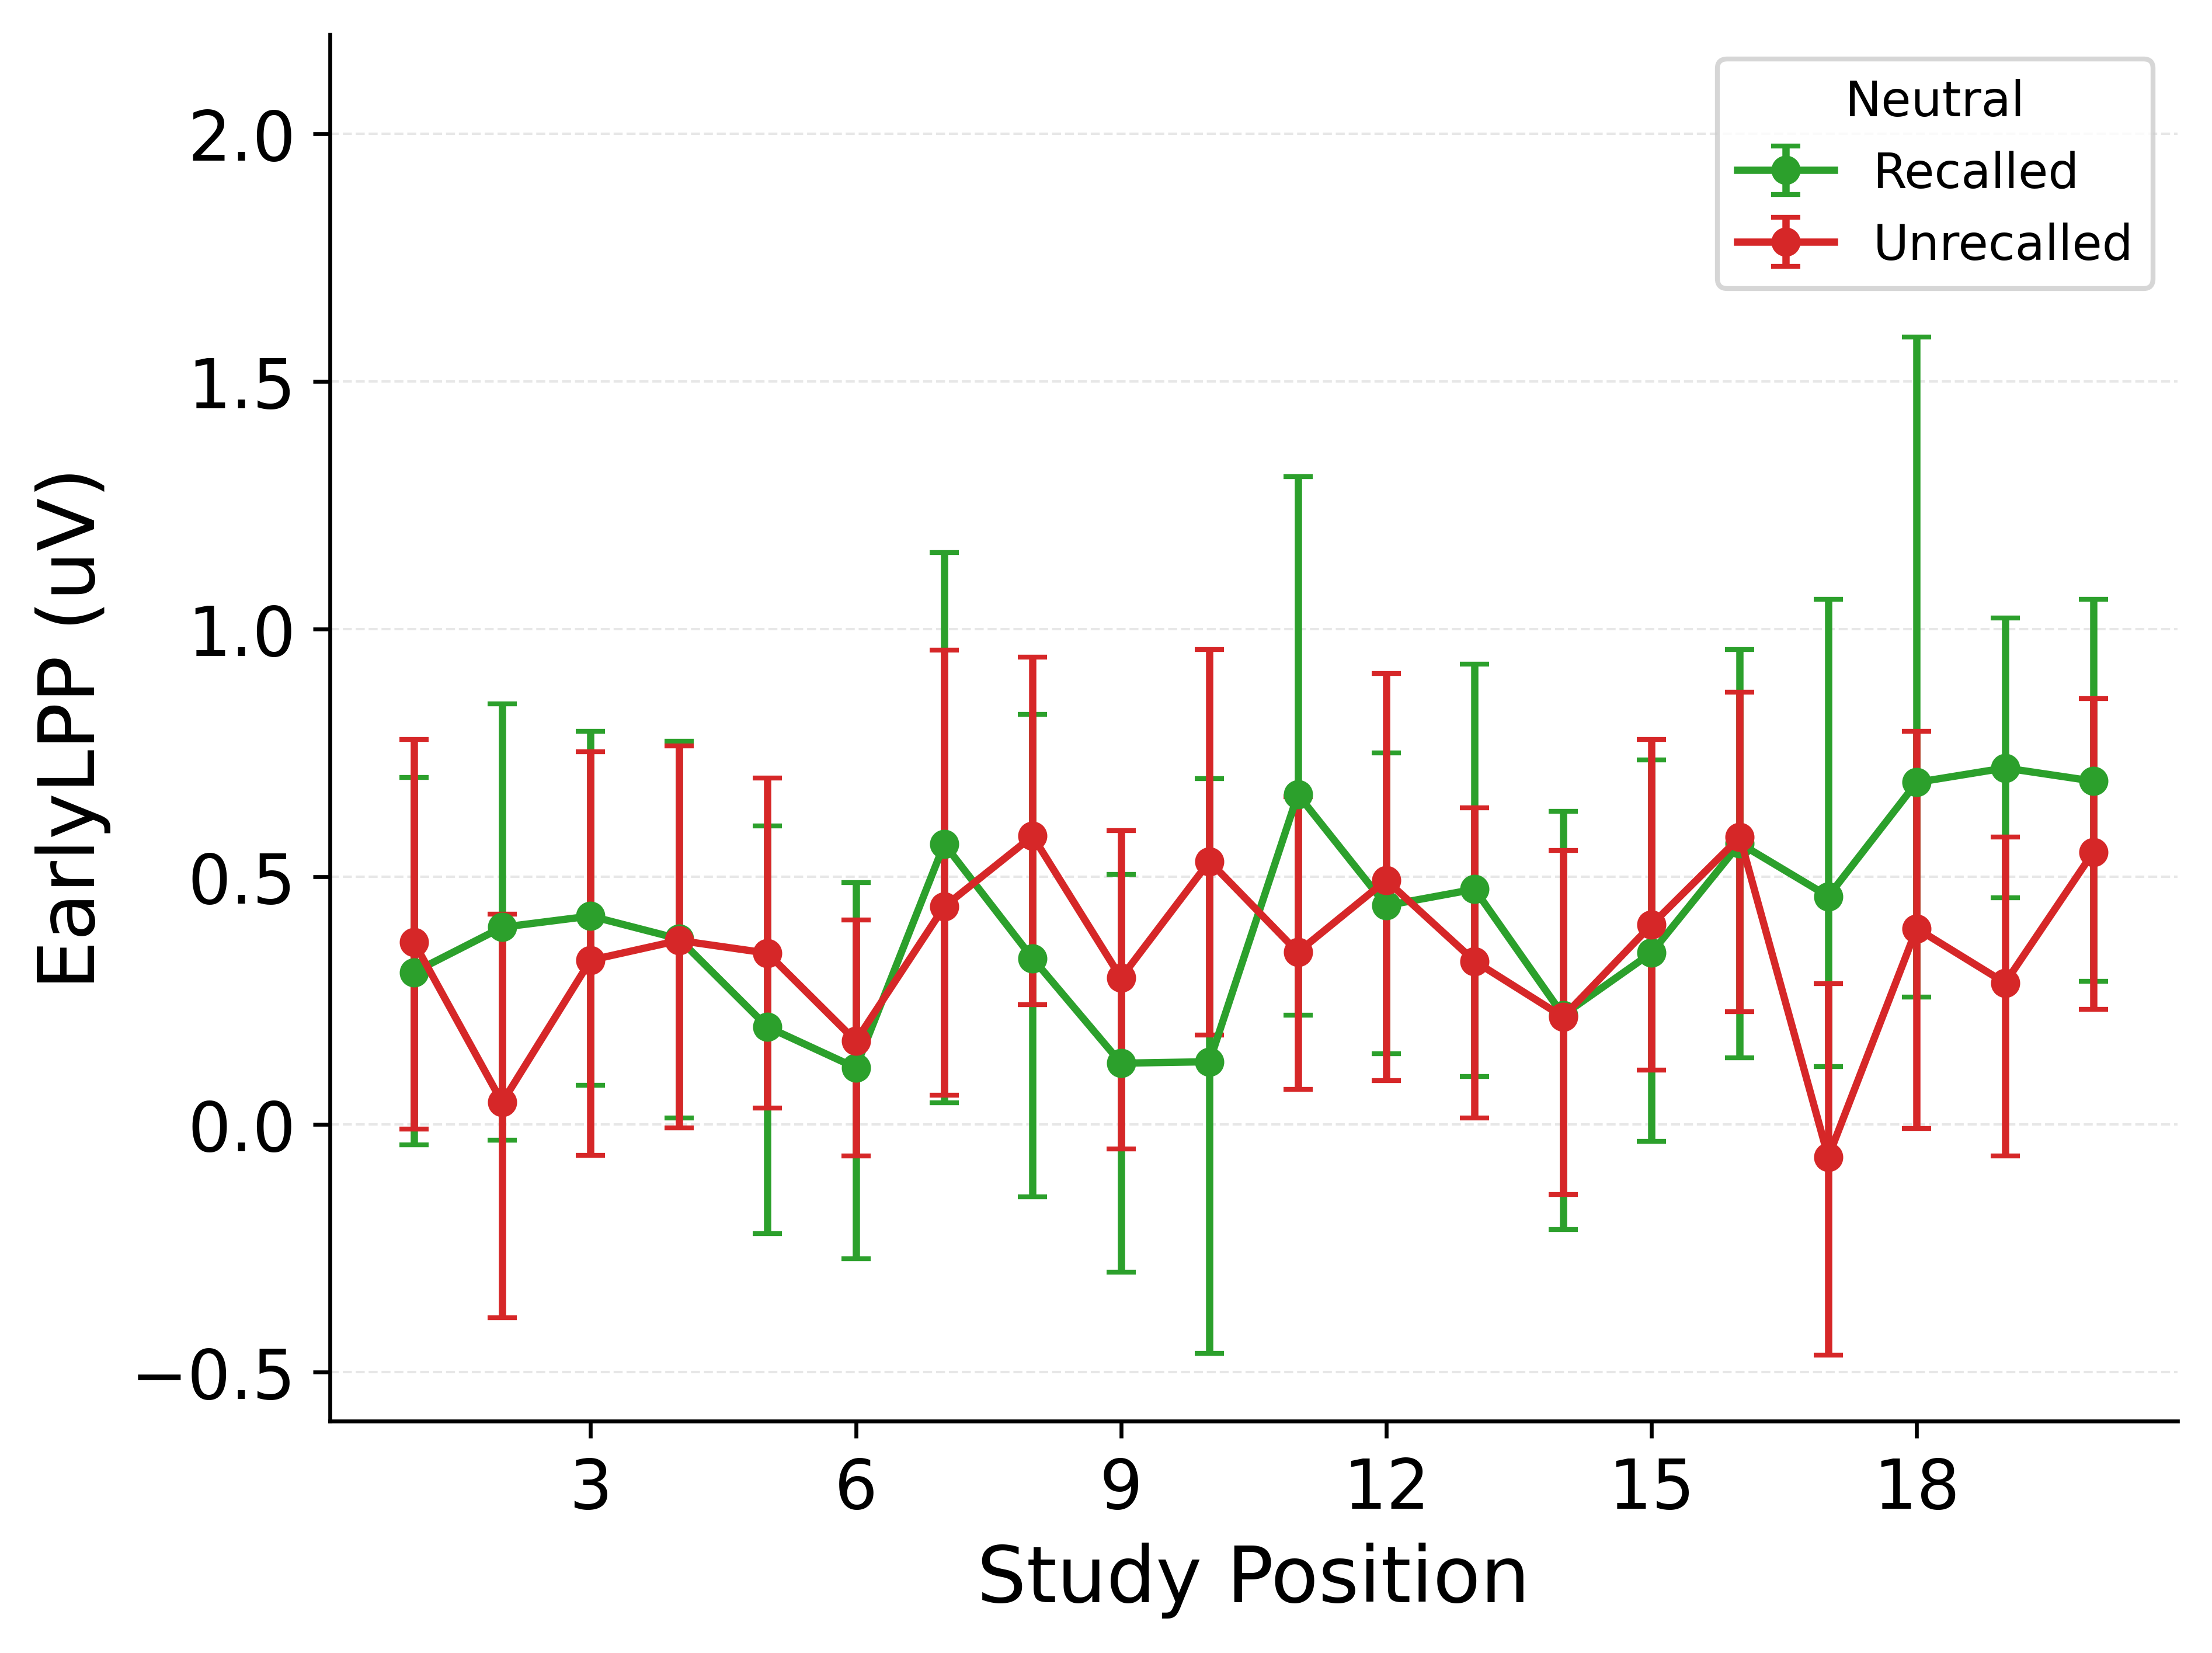
\includegraphics[keepaspectratio]{results/figures/analyses/cat_lpp_by_recall_EarlyLPP_Neutral.png}}\end{minipage}%
\newline
\begin{minipage}{0.50\linewidth}
\pandocbounded{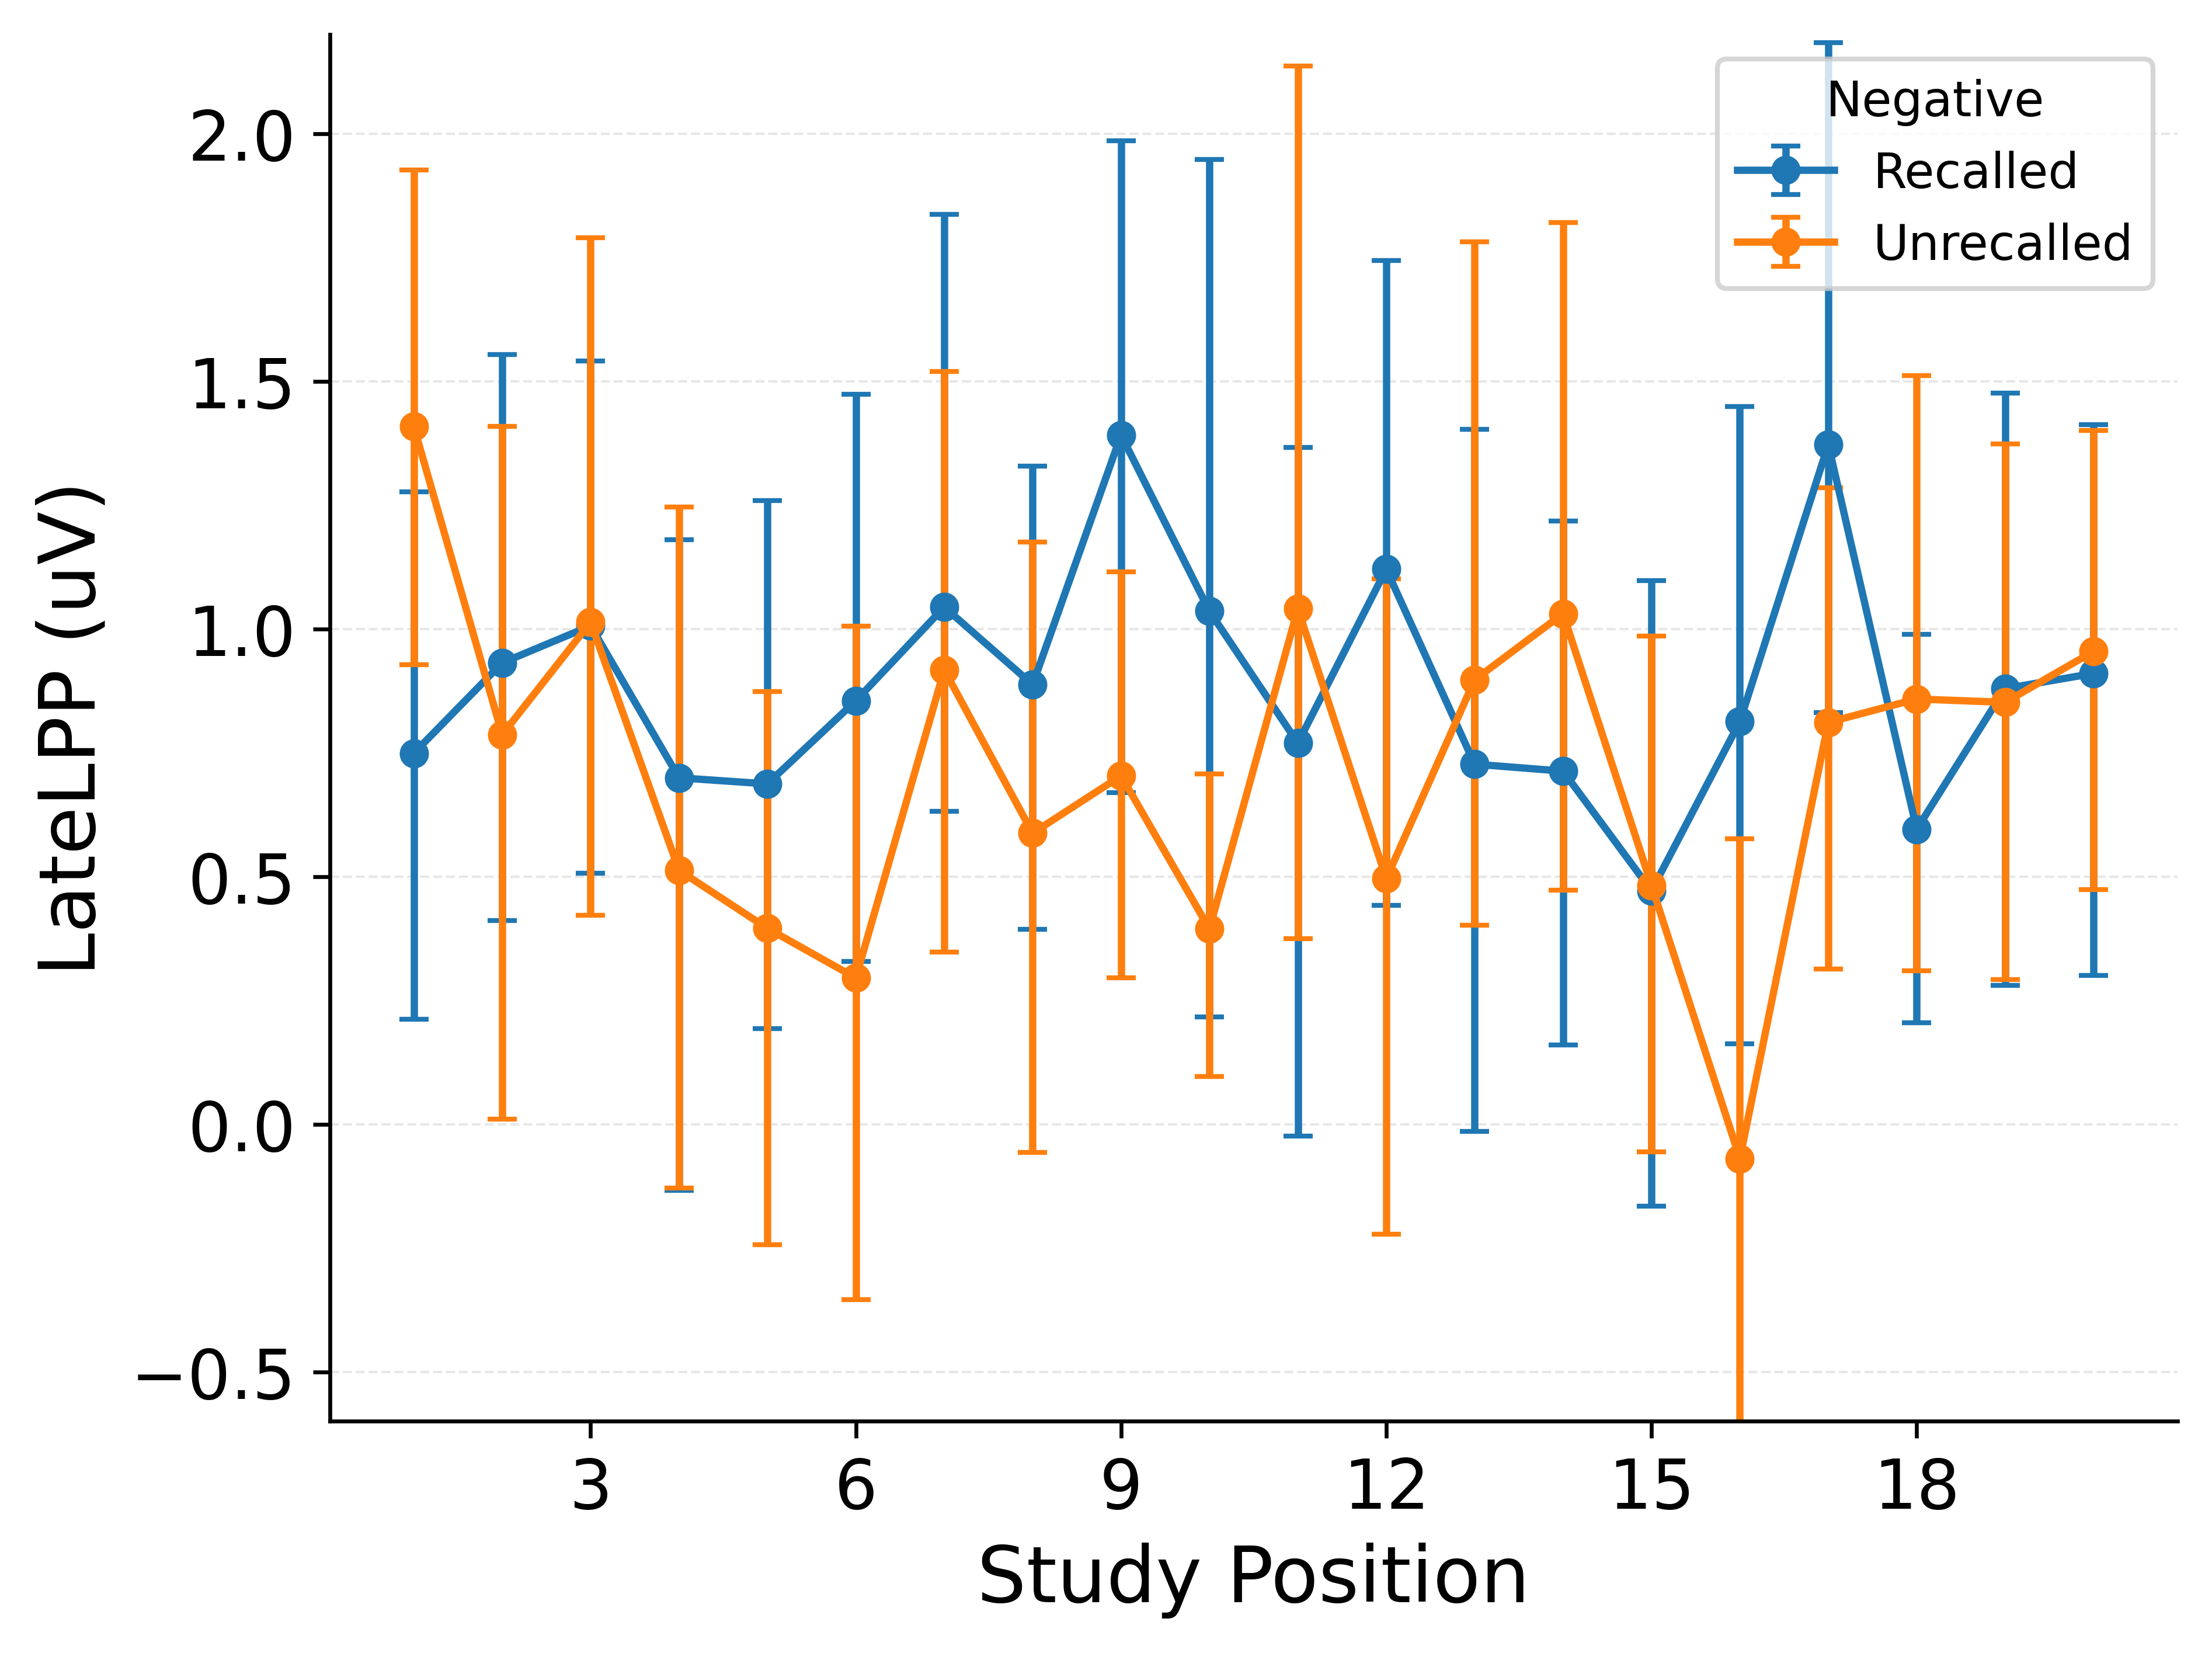
\includegraphics[keepaspectratio]{results/figures/analyses/cat_lpp_by_recall_LateLPP_Negative.png}}\end{minipage}%
%
\begin{minipage}{0.50\linewidth}
\pandocbounded{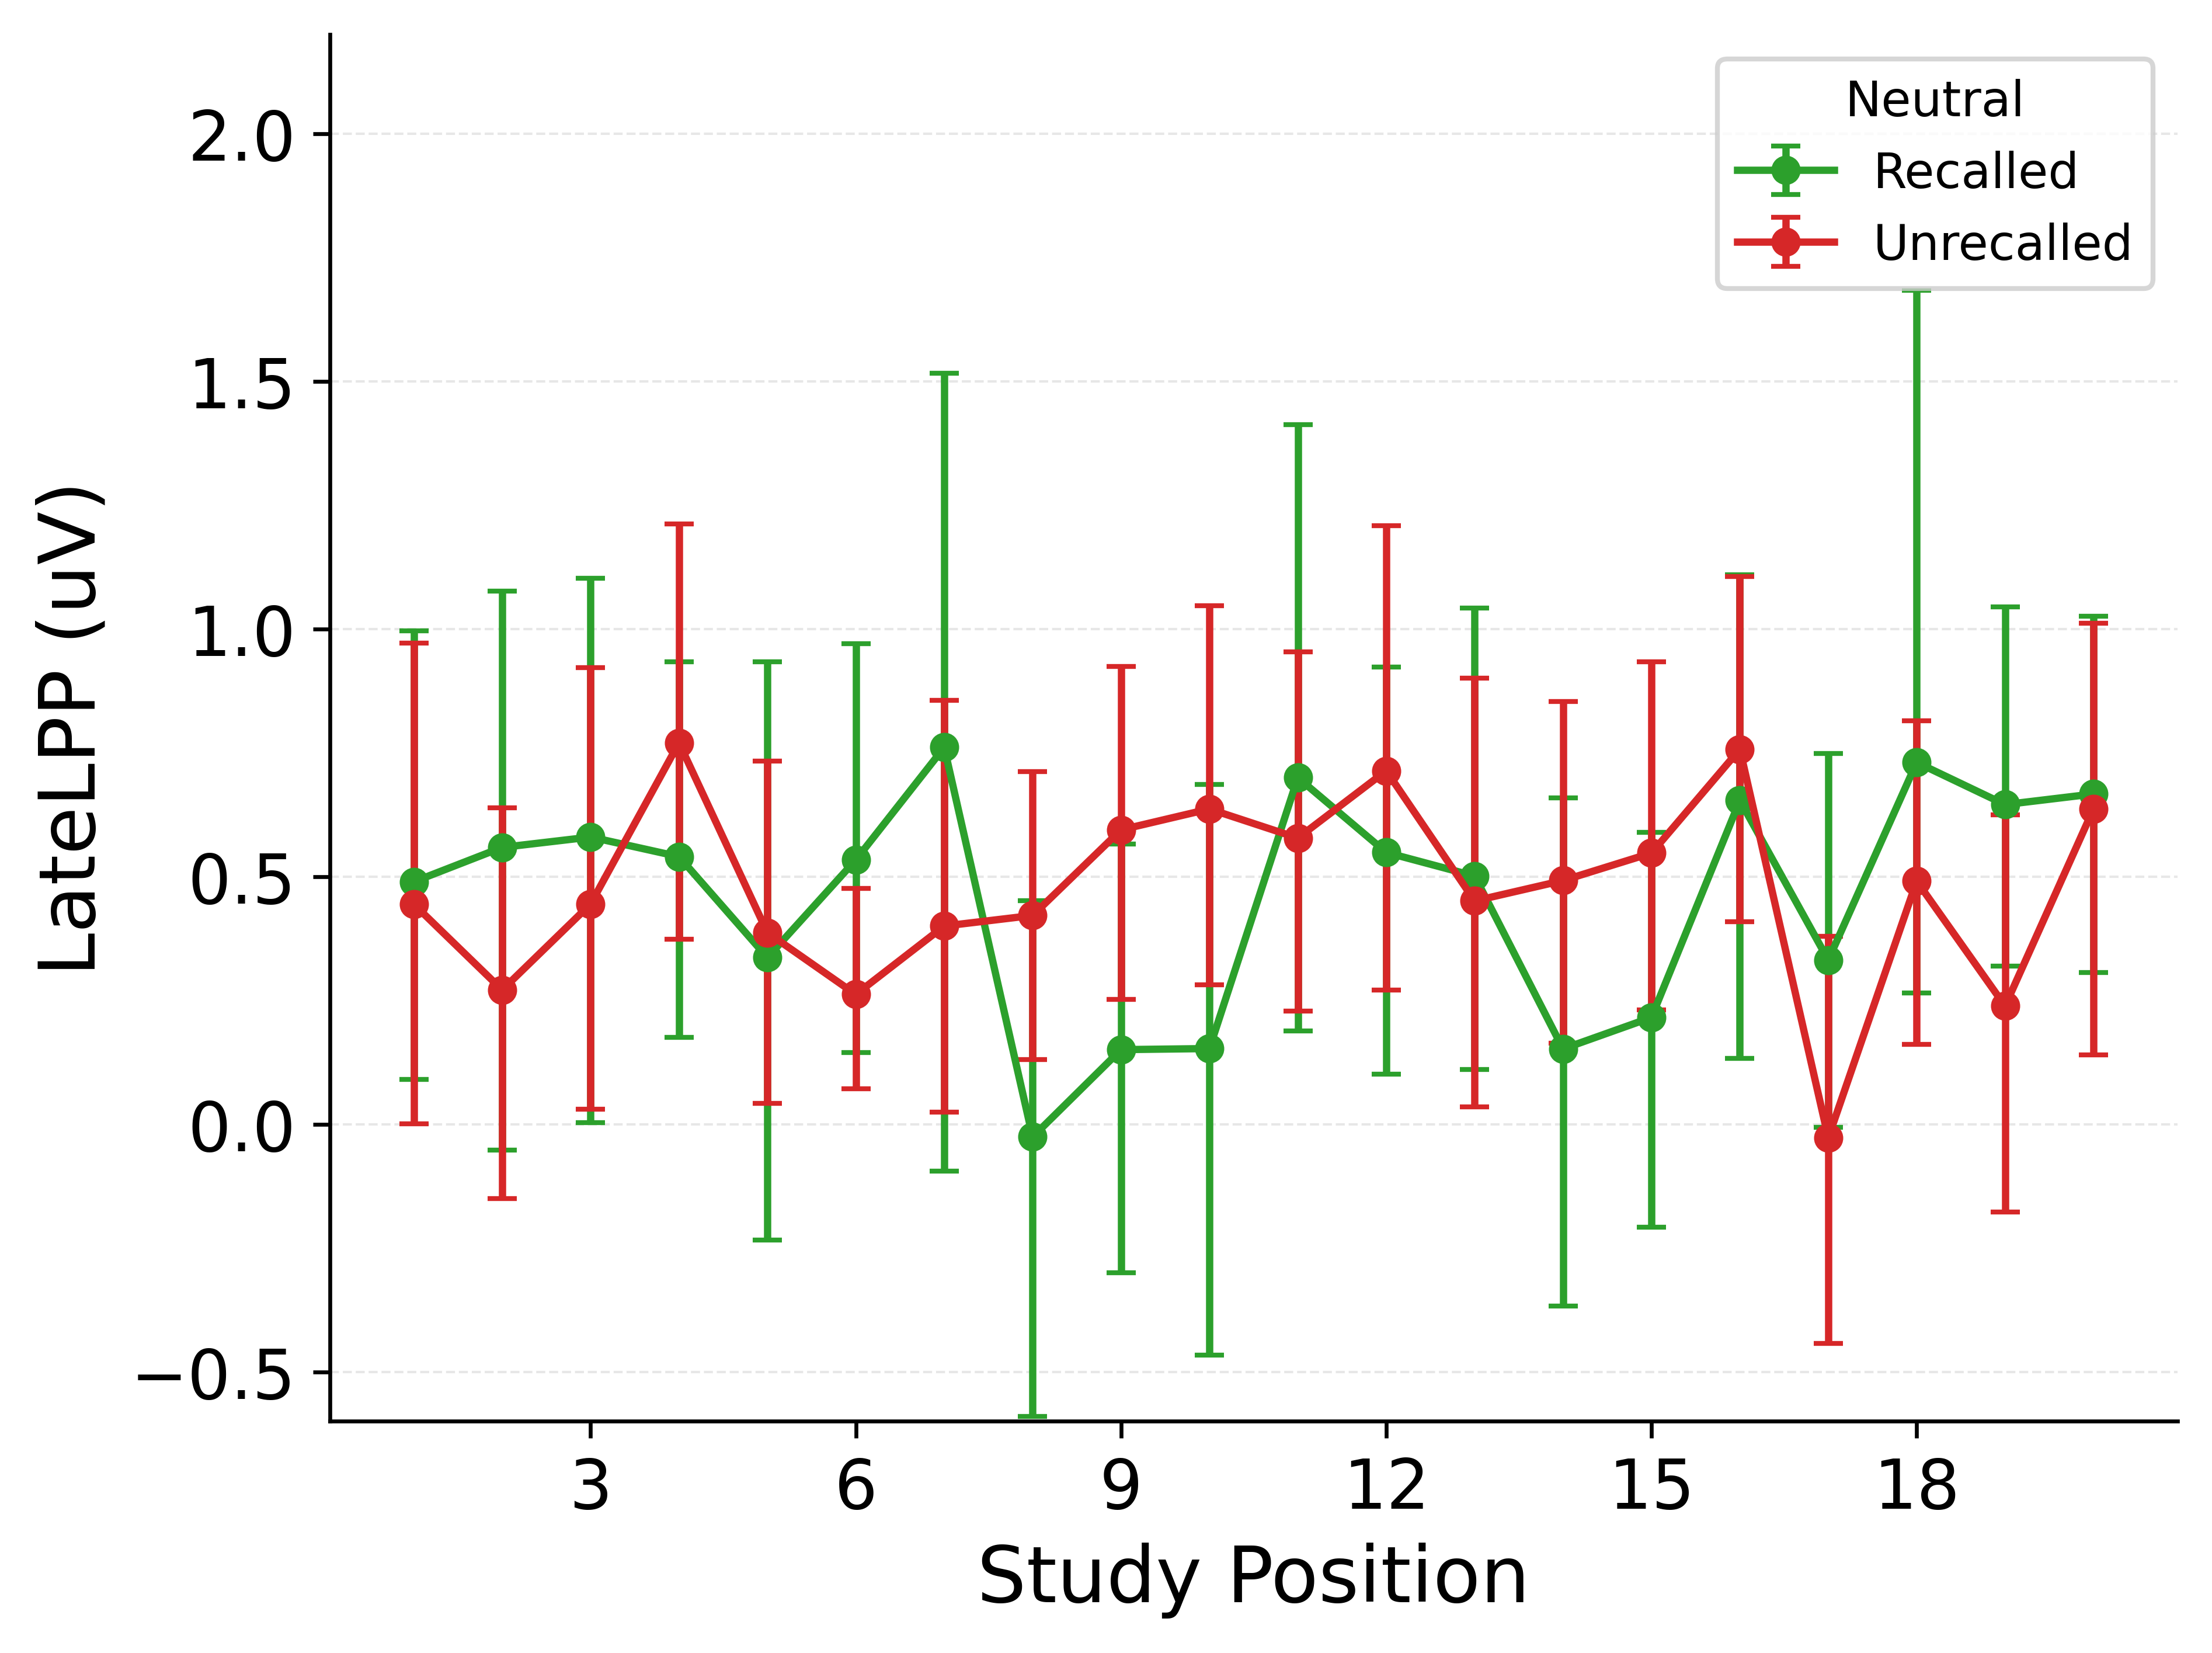
\includegraphics[keepaspectratio]{results/figures/analyses/cat_lpp_by_recall_LateLPP_Neutral.png}}\end{minipage}%

\end{figure}%

In Figure~\ref{fig-cat_lpp_by_recall}, we superimpose Early-LPP curves
to highlight joint structure. Recalled emotional items have the highest
Early LPPs. Unrecalled emotional items overlap with both recalled and
unrecalled neutral items. Two simple linking stories are inconsistent
with this pattern. First, if LPP simply reflected item type, recalled
and unrecalled items of the same type would have similar LPPs; instead,
recall status clearly separates Early LPP within the emotional
condition. Second, if LPP simply reflected recall probability, recalled
items across item types would align; instead, recalled emotional items
have higher LPPs than recalled neutral items. Neither pattern holds,
indicating an interaction between LPP and item type.

\begin{figure}

\caption{\label{fig-cat_lpp_by_recall}Early LPP by recall status and
item type. CIs omitted for clarity; data pooled across participants.}

\centering{

\pandocbounded{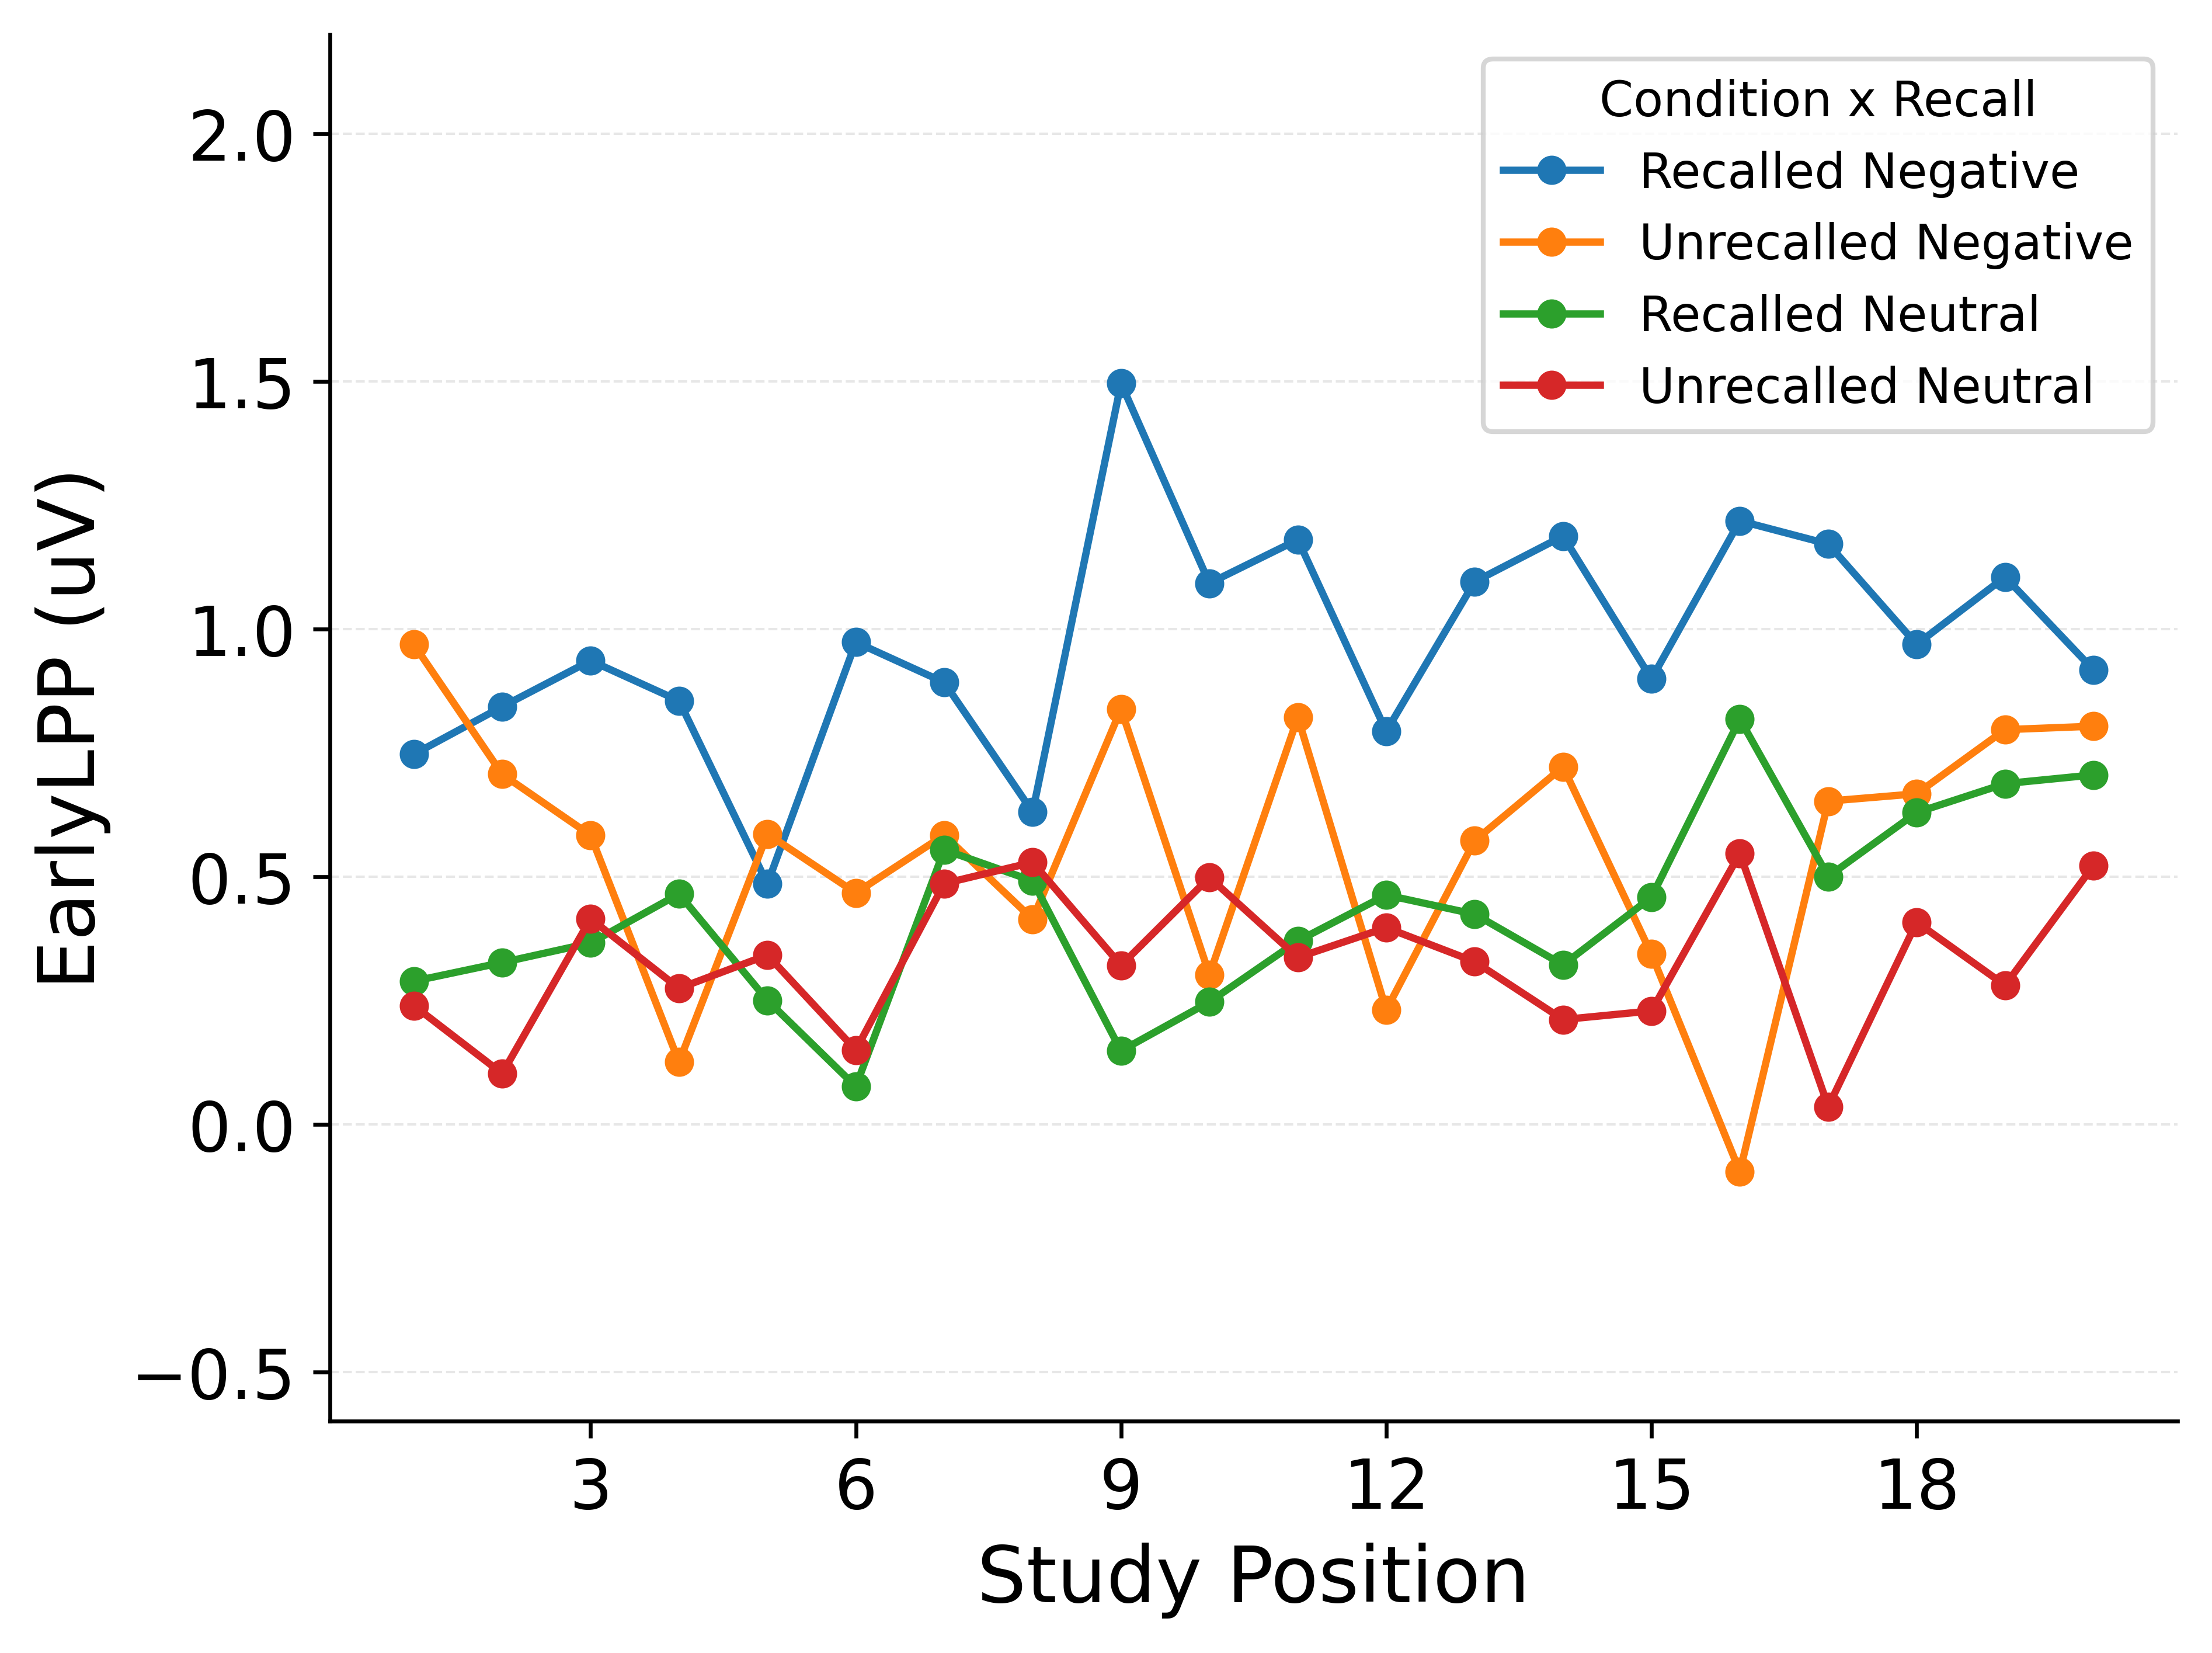
\includegraphics[keepaspectratio]{results/figures/cat_lpp_by_recall.png}}

}

\end{figure}%

We summarize Early-LPP contrasts with mean differences and 95\%
confidence intervals in Figure~\ref{fig-early-lpp-contrasts}. Recalled
emotional items sit significantly above every other group, and
unrecalled emotional items are elevated relative to unrecalled neutral
items, while recalled vs unrecalled neutral items do not differ
reliably. Together, these contrasts show that Early LPP peaks only when
emotion and later recall line up, reinforcing the interaction pattern
above.

\begin{figure}

\caption{\label{fig-early-lpp-contrasts}Early LPP contrasts (mean ΔµV
with 95\% CIs).}

\centering{

\begin{longtable*}[]{@{}
  >{\raggedright\arraybackslash}p{(\linewidth - 6\tabcolsep) * \real{0.4143}}
  >{\raggedright\arraybackslash}p{(\linewidth - 6\tabcolsep) * \real{0.2571}}
  >{\raggedright\arraybackslash}p{(\linewidth - 6\tabcolsep) * \real{0.2429}}
  >{\raggedright\arraybackslash}p{(\linewidth - 6\tabcolsep) * \real{0.0857}}@{}}
\toprule\noalign{}
\begin{minipage}[b]{\linewidth}\raggedright
Contrast
\end{minipage} & \begin{minipage}[b]{\linewidth}\raggedright
Δ Early LPP (µV)
\end{minipage} & \begin{minipage}[b]{\linewidth}\raggedright
95\% CI (µV)
\end{minipage} & \begin{minipage}[b]{\linewidth}\raggedright
Note
\end{minipage} \\
\midrule\noalign{}
\endhead
\bottomrule\noalign{}
\endlastfoot
E\_recalled -- E\_unrecalled & 0.43 & {[}0.27, 0.57{]} & sig. \\
E\_recalled -- N\_recalled & 0.55 & {[}0.37, 0.71{]} & sig. \\
E\_recalled -- N\_unrecalled & 0.64 & {[}0.50, 0.80{]} & sig. \\
E\_unrecalled -- N\_recalled & 0.12 & {[}-0.08, 0.31{]} & n.s. \\
E\_unrecalled -- N\_unrecalled & 0.22 & {[}0.06, 0.36{]} & sig. \\
N\_recalled -- N\_unrecalled & 0.10 & {[}-0.07, 0.28{]} & n.s. \\
\end{longtable*}

}

\end{figure}%

\subsubsection{Statistical Cross-Check}\label{statistical-cross-check}

Prior work using generalized mixed-effects models provides an
alternative perspective on these relationships.
Figure~\ref{fig-reference_gmm} predicts recall via a logistic link from
condition (emotional vs.~neutral), Early LPP, and their interaction. It
shows significant main effects of both factors and a significant
interaction. This aligns with the plots: a baseline recall advantage for
emotional items, an additional boost from early LPP, and a stronger LPP
effect for emotional items than for neutral items.

\begin{figure}

\caption{\label{fig-reference_gmm}Description of a generalized mixed
effects model predicting recall as a function of condition, earlyLPP,
and their interaction.}

\centering{

\pandocbounded{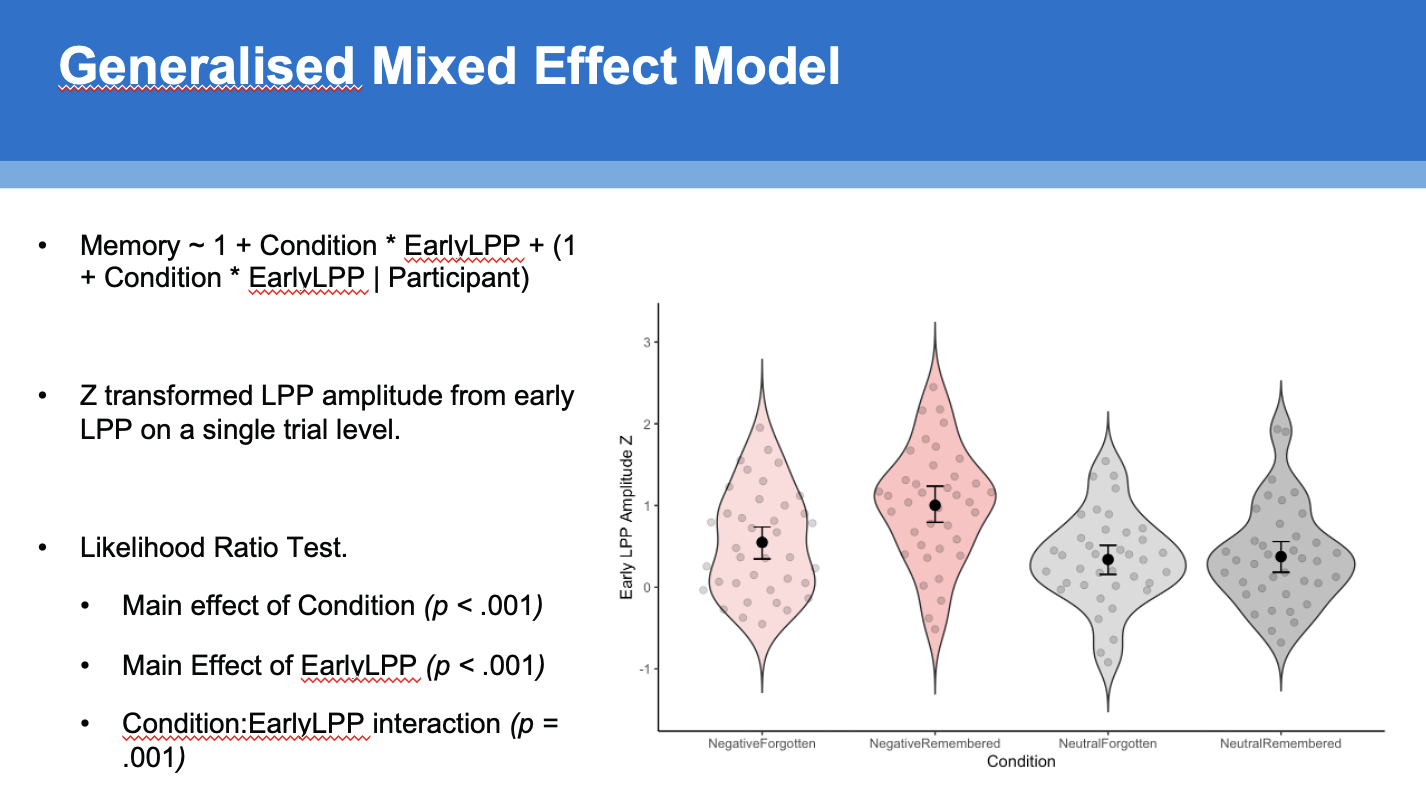
\includegraphics[keepaspectratio]{results/figures/reference_gmm.png}}

}

\end{figure}%

\subsection{Recall Sets Show Little to No Temporal
Clustering}\label{recall-sets-show-little-to-no-temporal-clustering}

Classic work on free recall shows that successive recalls tend to come
from nearby study positions, a temporal contiguity effect. Standard
analyses quantify this with the lag-conditional response probability
(lag-CRP), which requires recall order. Because recall order is
unavailable in the present EEG dataset, we developed an order-agnostic
alternative that asks a closely related question: given that a studied
item was recalled, how likely is it that items at nearby study positions
were also recalled?

For each list, each recalled item at position \(i\), and each absolute
lag \(d = 1,\dots,19\), we examine the item at position \((i+d)\) (when
it exists) and estimate the conditional co-recall probability,

\[
\text{CoRec}(d) = P(r_{i+d}=1 \mid r_i=1,\ |j-i|=d),
\]

as the probability that the item at lag \(d\) is recalled given that the
reference item at position \(i\) is recalled. Averaging
\(\text{CoRec}(d)\) across lists yields an order-agnostic temporal
contiguity curve that parallels the lag-CRP but does not require output
sequences.

To validate this measure, we first applied it to a dataset where recall
order is available. For this comparison we used a subset of PEERS
(\citeproc{ref-healey2014memory}{Healey \& Kahana, 2014}): 126
participants aged 17--30 completed 112 trials in which they studied
lists of 16 unique words and then immediately recalled them. Words were
sampled without replacement from the Toronto Word Pool
(\citeproc{ref-friendly1982toronto}{Friendly et al., 1982}), a set of
high-frequency nouns, adjectives, and verbs with low interitem
similarity. The left panel of Figure~\ref{fig-peers_lagcrp_condcorec}
shows the standard lag-CRP for this dataset, with a strong contiguity
effect: recall transitions are most likely at lag +1, somewhat less
likely at lag −1, and fall off rapidly for larger \(|lag|\). The right
panel shows the corresponding conditional co-recall curve
\(\text{CoRec}(d)\), collapsed over lag sign. Conditional co-recall is
highest for short lags and decreases steadily with distance, closely
mirroring the lag-CRP gradient despite ignoring recall order. These
results confirm that the conditional co-recall analysis is sensitive to
temporal contiguity when it is present.

\begin{figure}

\caption{\label{fig-peers_lagcrp_condcorec}Standard lag-CRP (LEFT) and
order-agnostic conditional co-recall by lag (RIGHT) for a subset of the
PEERS dataset (\citeproc{ref-healey2014memory}{Healey \& Kahana, 2014}).
The conditional co-recall curve reproduces the short-lag advantage
observed in the lag-CRP despite not using recall order information.}

\begin{minipage}{0.50\linewidth}
\pandocbounded{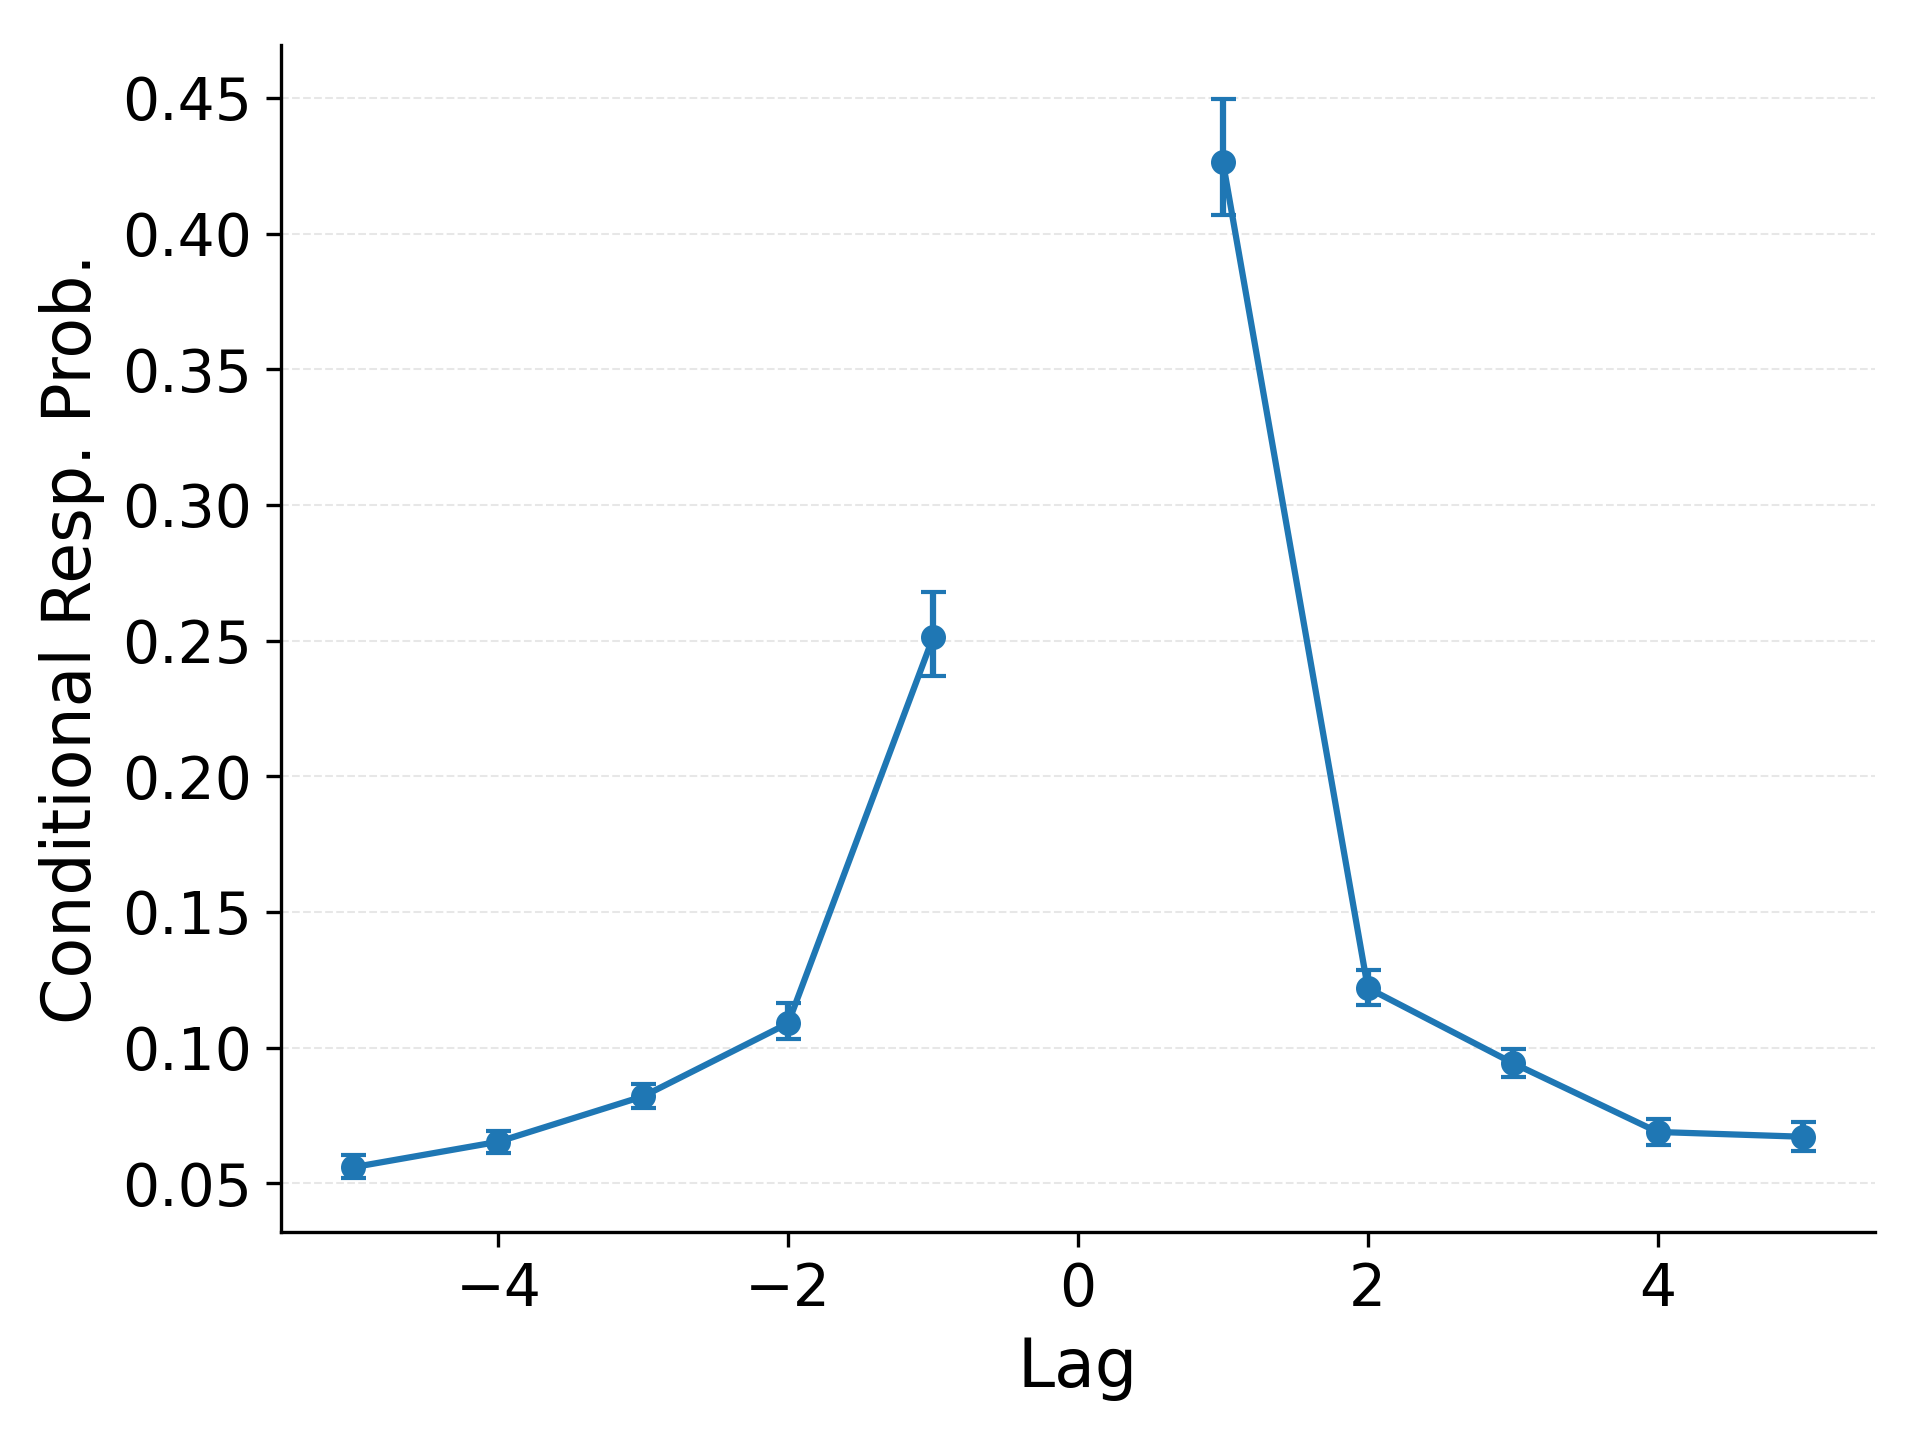
\includegraphics[keepaspectratio]{results/figures/analyses/peers_lagcrp.png}}\end{minipage}%
%
\begin{minipage}{0.50\linewidth}
\pandocbounded{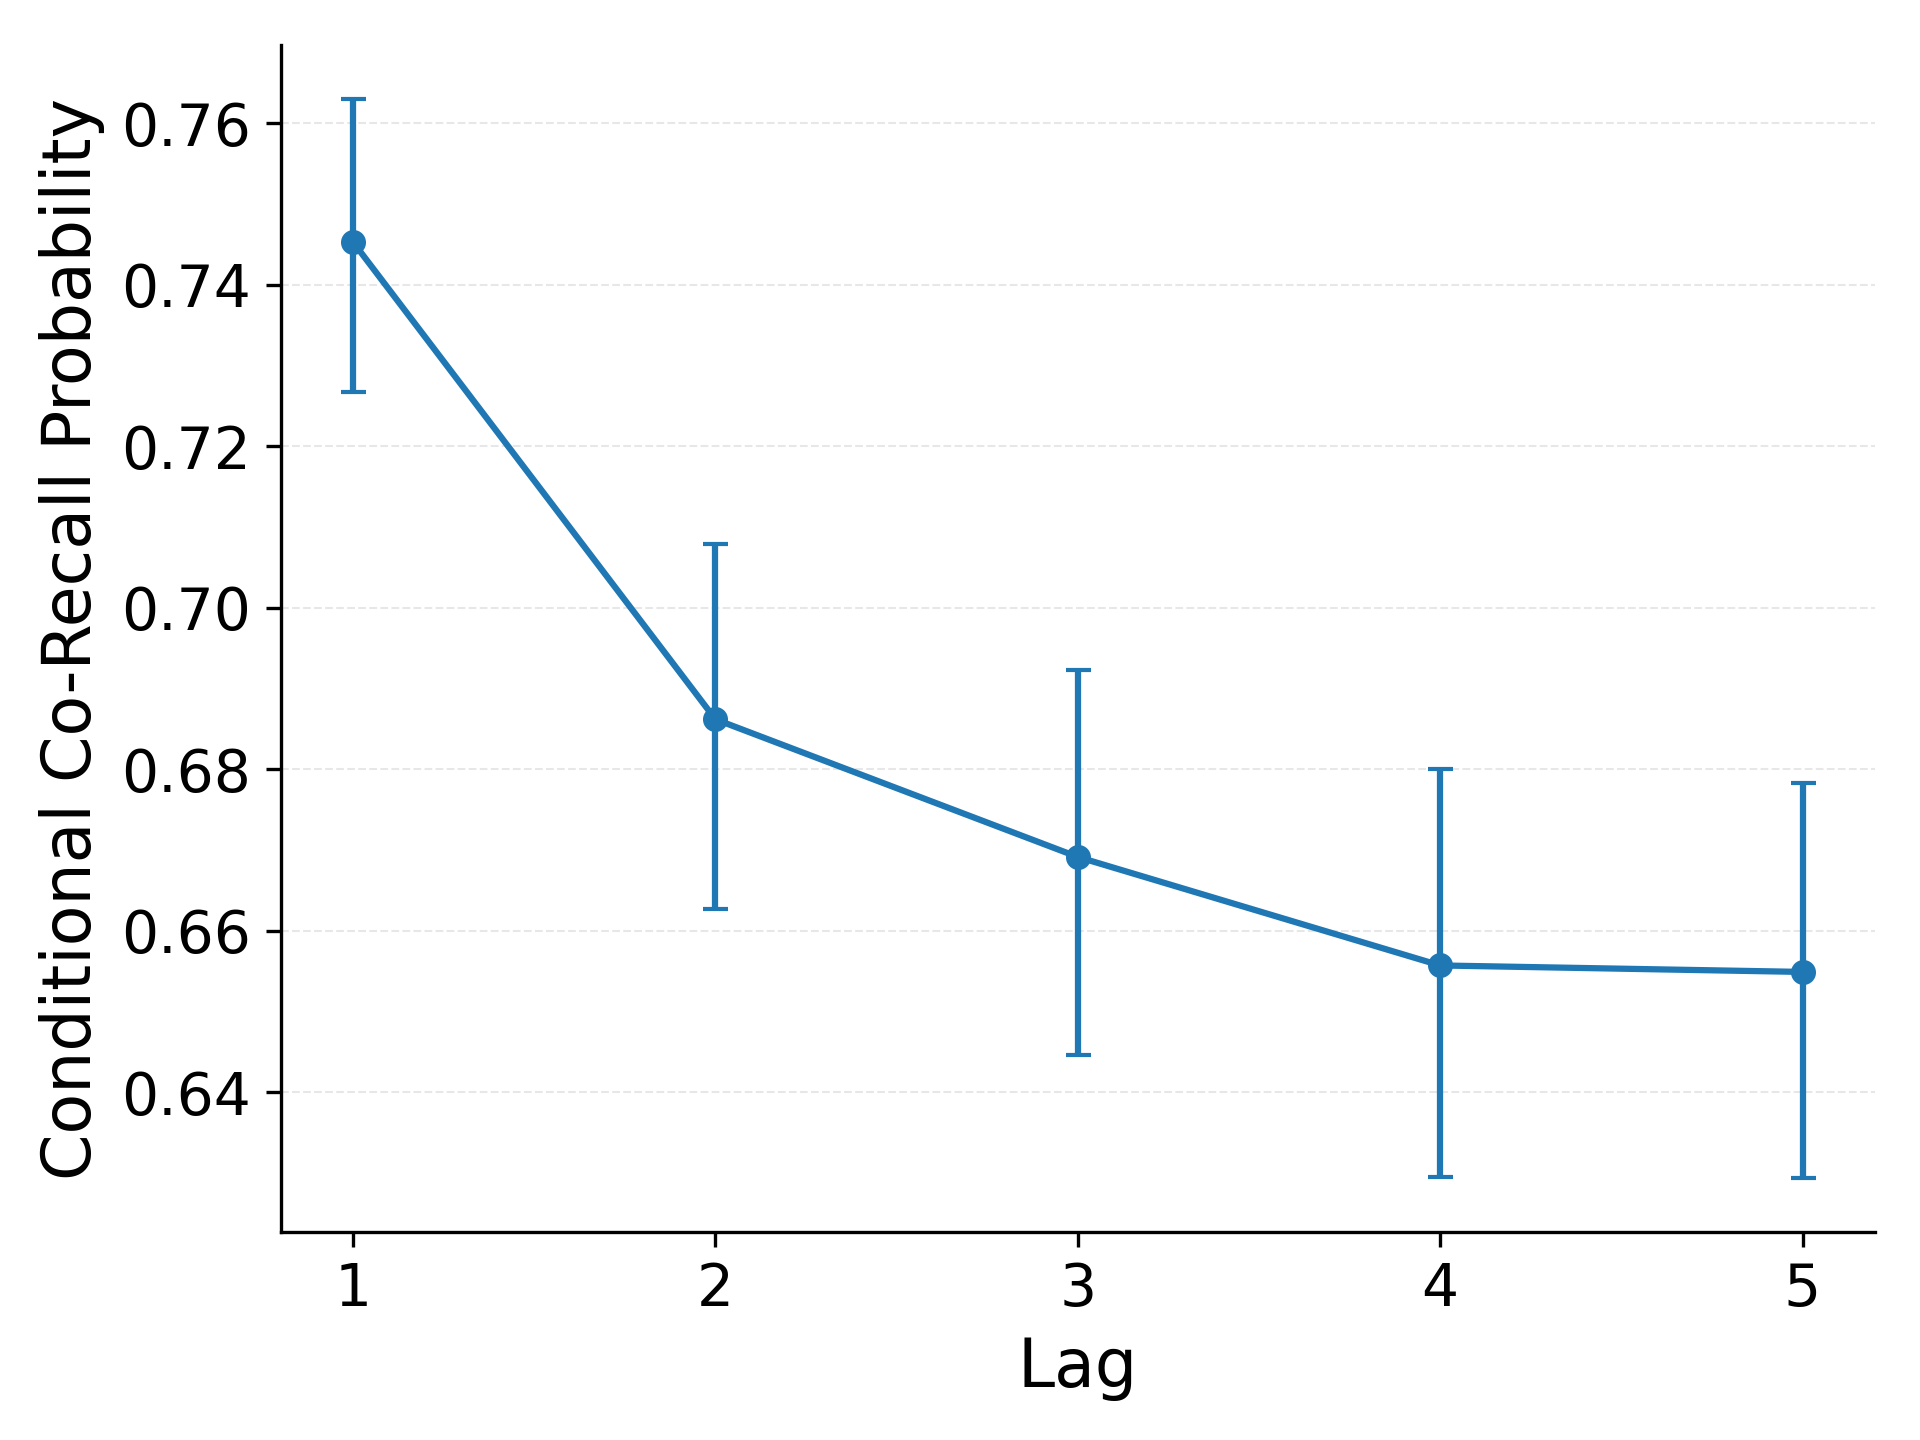
\includegraphics[keepaspectratio]{results/figures/analyses/peers_condcorec_by_lag.png}}\end{minipage}%

\end{figure}%

We then applied the same conditional co-recall analysis to the Zarubin
EEG dataset. As shown in Figure~\ref{fig-zarubin_condcorec_by_lag}, the
conditional co-recall curve is nearly flat: items at lag 1 are only
slightly more likely to be recalled than items at lags 4-5, and the
difference is small relative to the bootstrap confidence intervals. In
contrast to the PEERS subset, this paradigm therefore shows at most a
weak temporal contiguity effect in recall sets and provides only limited
constraint on the temporal-context dynamics in our models.

\begin{figure}

\caption{\label{fig-zarubin_condcorec_by_lag}Order-agnostic conditional
co-recall by lag for the Zarubin EEG dataset. Conditional co-recall
probabilities vary little with lag, indicating weak temporal clustering
of recalled items in this paradigm.}

\centering{

\pandocbounded{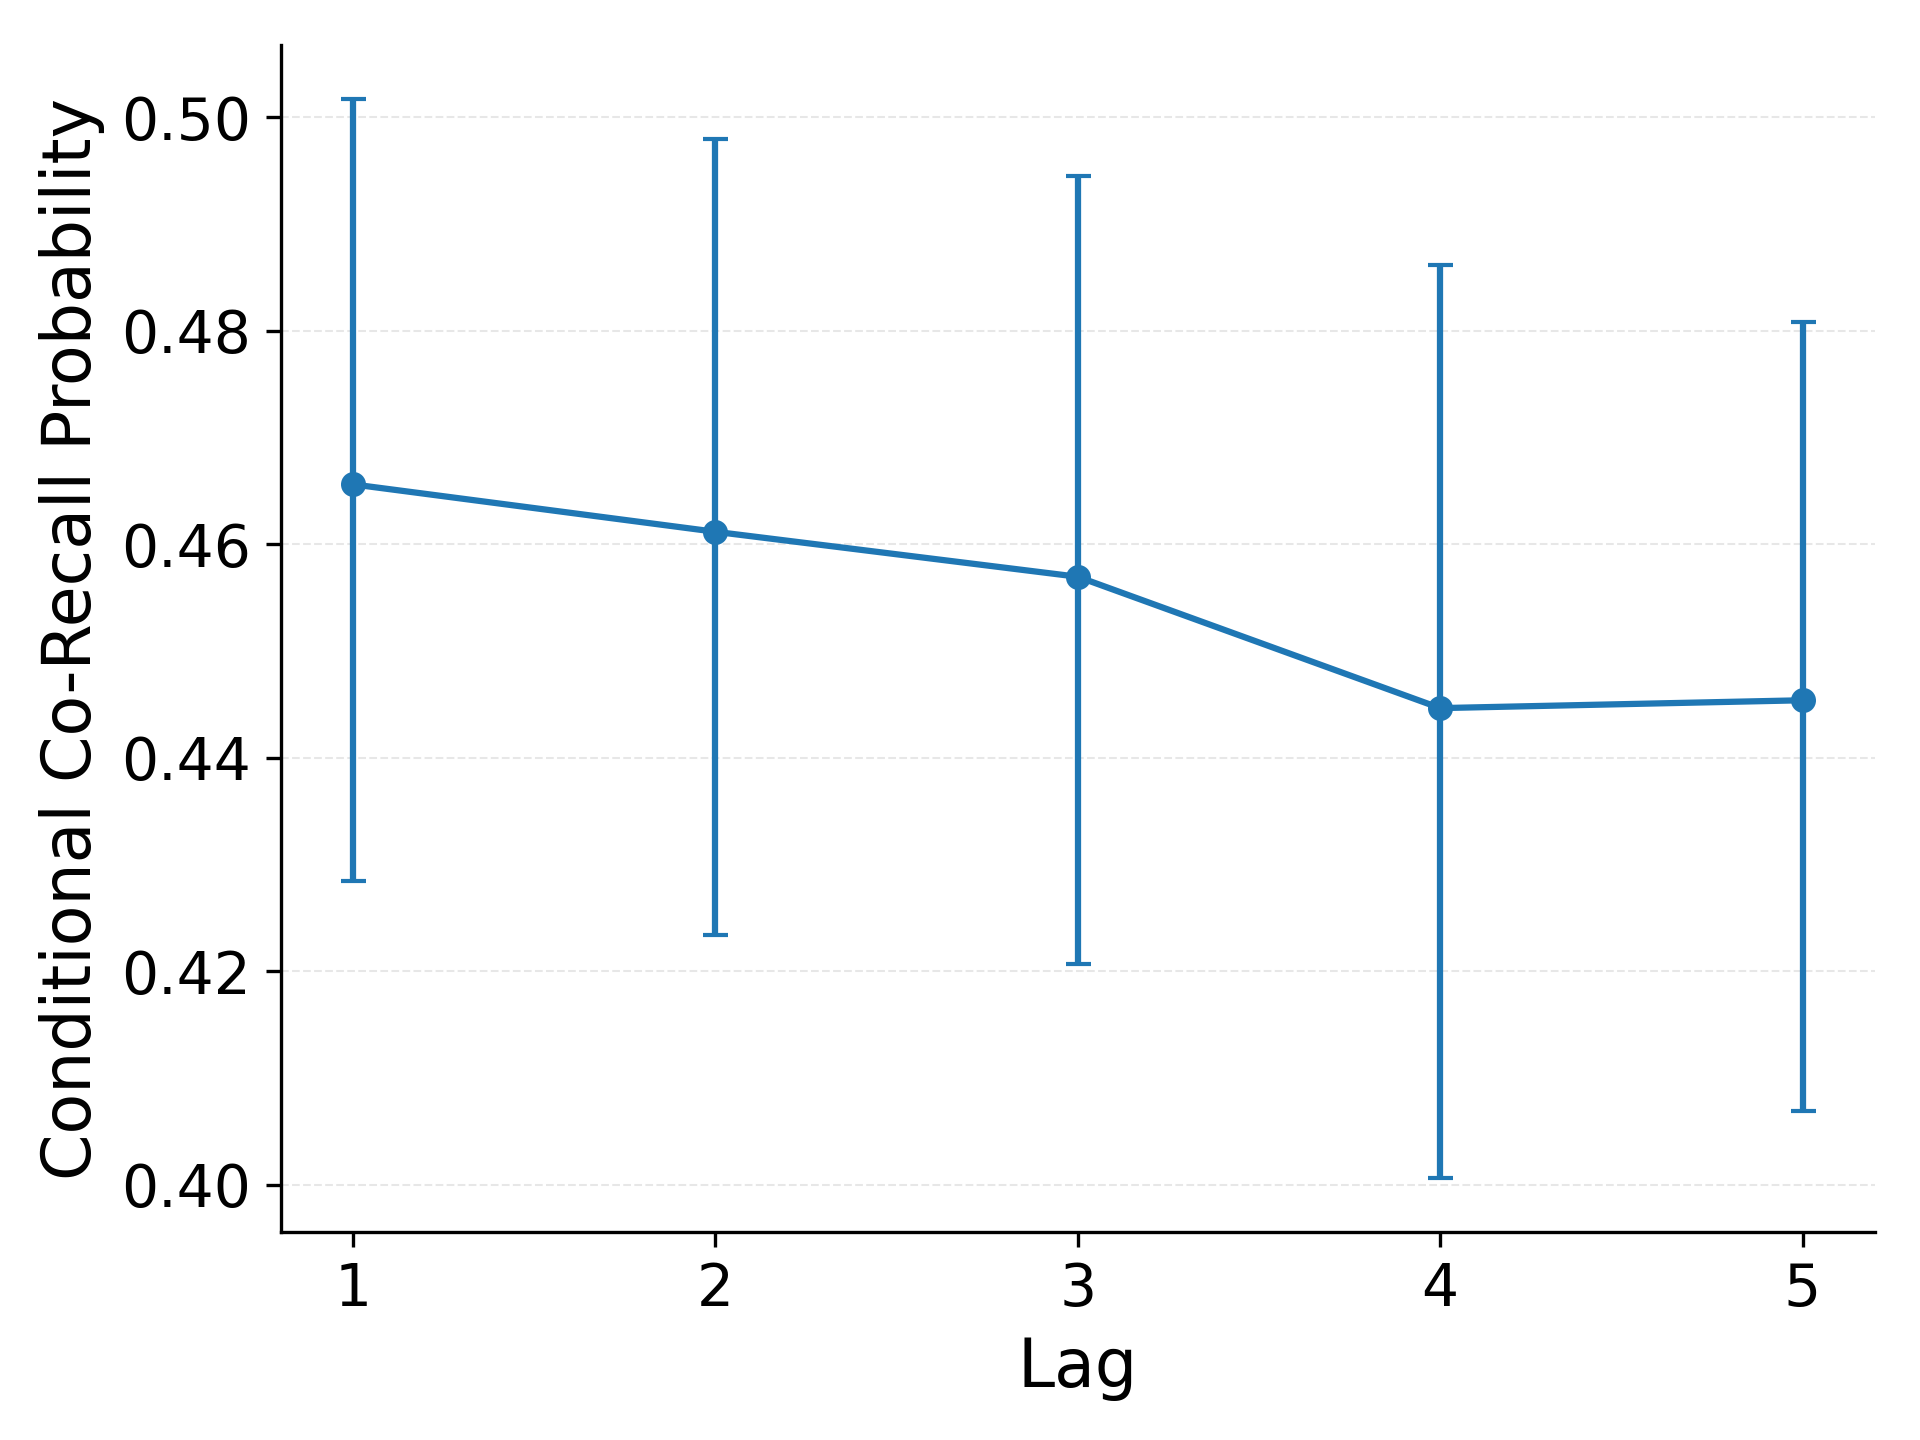
\includegraphics[keepaspectratio]{results/figures/analyses/zarubin_condcorec_by_lag.png}}

}

\end{figure}%

\section{Modeling Strategy}\label{modeling-strategy}

Taken together, these benchmarks place clear constraints on any
mechanistic account of how LPP relates to emotion and memory. Item type
and LPP must be treated as distinct inputs whose effects interact:
emotional items enjoy a baseline recall advantage (EEM), and Early LPP
further modulates recall likelihood, with a much stronger association
for emotional items than for neutral items. The mixed-effects
cross-check confirms this pattern, showing main effects of condition and
Early LPP as well as a significant interaction.

The joint pattern in Figure~\ref{fig-cat_lpp_by_recall} and
Figure~\ref{fig-cat_lpp_by_recall_split} rules out LPP as a pure emotion
tag or a pure recall tag: recalled emotional items sit highest, while
unrecalled emotional items overlap with neutral items across recall
status. Collapsing LPP into a single signal would mispredict either
unrecalled emotional items or recalled neutral items.

Our conditional co-recall analysis is the only benchmark that directly
targets temporal context. It reproduces a strong contiguity gradient in
PEERS but is nearly flat in the Zarubin EEG dataset, indicating weak
temporal clustering and limited constraint on temporal-context dynamics.
Given the task design, strong semantic and emotional clustering may
compete with temporal context, so we avoid strong claims about
temporal-context mechanisms here.

These constraints motivate treating item type and LPP as interacting
influences on encoding or retrieval while keeping temporal context
effects modest in scope. The mixed-effects cross-check supports this
view (main effects plus interaction) but does not specify how the
predictors should enter an encoding rule or propagate through
retrieved-context dynamics to shape recall sets.

In the next section, we focus on three closely related eCMR variants
that directly address whether LPP adds explanatory value beyond emotion
labels and whether that value differs by item type. We compare an
emotion-only model (no LPP input), a model with a single LPP slope
shared across items, and a model with an additional LPP slope for
emotional items. These comparisons test whether LPP contributes
incremental information about recall sets and whether the GMM-style
interaction requires an explicit emotion-dependent term or can arise
from retrieved-context dynamics.

\subsection{eCMR Specification}\label{ecmr-specification}

We use a connectionist CMR architecture with a temporal context and
implement emotion and LPP as modulators of learning strength rather than
a separate emotional context state. This simplified eCMR is appropriate
here because the dataset provides no recall-order scaffold to validate
an explicit emotional context trajectory. It also yields a cleaner
comparison across emotion-only, LPP main-effects, and LPP interaction
models by placing LPP in a common learning pathway rather than different
loci for neutral versus emotional items. We denote temporal context as
\(c^T\), with item features \(f_i\). The matrix \(M^{FC}\) binds item
features to temporal context, and \(M^{CF}\) binds temporal context to
item features.

\begin{table}

{\caption{{Parameters and structures specifying
eCMR.}{\label{tbl-ecmr-parameters}}}
\vspace{-20pt}}

\begin{longtable}[]{@{}
  >{\raggedright\arraybackslash}p{(\linewidth - 4\tabcolsep) * \real{0.3333}}
  >{\raggedright\arraybackslash}p{(\linewidth - 4\tabcolsep) * \real{0.3333}}
  >{\raggedright\arraybackslash}p{(\linewidth - 4\tabcolsep) * \real{0.3333}}@{}}
\toprule\noalign{}
\begin{minipage}[b]{\linewidth}\raggedright
Symbol
\end{minipage} & \begin{minipage}[b]{\linewidth}\raggedright
Name
\end{minipage} & \begin{minipage}[b]{\linewidth}\raggedright
Description
\end{minipage} \\
\midrule\noalign{}
\endhead
\bottomrule\noalign{}
\endlastfoot
\(c^T\) & temporal context & Recency-weighted summary of prior items. \\
\(f_i\) & item features & One-hot representation of item \(i\). \\
\(M^{FC}\) & item-to-temporal-context memory & Feature-to-context
associations. \\
\(M^{CF}\) & context-to-item memory & Temporal context cueing item
features. \\
\(\beta_{enc}\) & encoding drift rate & Integration rate of temporal
context during encoding. \\
\(\beta_{start}\) & start drift rate & Start-list context integration at
recall onset. \\
\(\beta_{rec}\) & recall drift rate & Integration rate of temporal
context during recall. \\
\(\alpha\) & shared support & Uniform pre-experimental support in
\(M^{CF}\). \\
\(\delta\) & item support & Self-support in \(M^{CF}\). \\
\(\gamma\) & learning rate & Feature-to-context learning rate in
\(M^{FC}\). \\
\(\phi_s\) & primacy scale & Initial boost to \(M^{CF}\) learning. \\
\(\phi_d\) & primacy decay & Decay rate of the primacy boost. \\
\(\tau_c\) & choice sensitivity & Exponent for Luce-style
competition. \\
\(\phi_{emot}\) & emotional learning boost & Value is \(\phi_{emot}\)
for emotional items and 0 for neutral items. \\
\(L_i\) & centered Early LPP & List-centered Early LPP for item
\(i\). \\
\(\kappa_L\) & LPP main scale & Slope for LPP main effect. \\
\(\lambda_L\) & LPP main threshold & Centering offset for the LPP main
effect. \\
\(\kappa_{EL}\) & LPP interaction scale & Slope for LPP-by-emotion
interaction. \\
\(\lambda_{EL}\) & LPP interaction threshold & Centering offset for the
interaction term. \\
\end{longtable}

\end{table}

Temporal context uses the standard CMR pre-experimental initializations:

\[
M^{FC}_{pre(ij)} =
\begin{cases}
1 - \gamma & \text{if } i=j \\
0 & \text{if } i \neq j
\end{cases}
\]

\[
M^{CF}_{pre(ij)} =
\begin{cases}
\delta & \text{if } i=j \\
\alpha & \text{if } i \neq j
\end{cases}
\]

Here, \(\gamma\) scales the ratio of new feature-to-context associations
formed during the experiment to pre-experimental item--context links.
The parameters \(\delta\) and \(\alpha\) set pre-experimental
self-support and shared support in context-to-feature memory,
respectively. During encoding, temporal contextual input is retrieved as
\(c^{IN}_i = M^{FC} f_i\) and normalized to unit length. Temporal
context updates according to:

\[
c^T_i = \rho_i c^T_{i-1} + \beta_{enc} c^{IN}_i
\]

\[
\rho_i = \sqrt{1 + \beta_{enc}^2\left[\left(c^T_{i-1} \cdot c^{IN}_i\right)^2 - 1\right]} - \beta_{enc}\left(c^T_{i-1} \cdot c^{IN}_i\right)
\]

Here, \(\beta_{enc}\) sets the drift rate of temporal context during
encoding and \(\rho_i\) normalizes the context vector.
Feature-to-context learning uses a Hebbian update:

\[
\Delta M^{FC}_{ij} = \gamma f_i c^T_j
\]

This update uses \(\gamma\) as the feature-to-context learning rate.
Primacy is implemented by scaling the temporal context-to-feature
learning rate:

\[
\phi_i = \phi_s e^{-\phi_d(i-1)} + 1
\]

Here, \(\phi_s\) sets the initial primacy boost and \(\phi_d\) controls
its decay across serial positions. Learning strength is defined as:

\[
g_i = \phi_{emot,i} + \phi_i
\]

Here, \(\phi_{emot,i}\) equals \(\phi_{emot}\) for emotional items and 0
for neutral items. The primacy term \(\phi_i\) enters additively to
capture an independent primacy contribution to learning strength.
Context-to-feature learning uses the learning strength \(g_i\):

\[
\Delta M^{CF}_{ij} = g_i c^T_j f_i
\]

This update uses \(g_i\) to bind items in \(M^{CF}\). At the start of
recall, temporal context is shifted toward the pre-list state:

\[
c^T_{start} = \rho_{N+1} c^T_N + \beta_{start} c^T_0
\]

Here, \(\beta_{start}\) controls how much start-list context is
reinstated at retrieval onset. At each recall step, temporal context
cues item activations:

\[
A = M^{CF} c^T
\] At each recall step, the probability of recalling item \(i\) is:

\[
P(i) = \frac{A_i^{\tau_c}}{\sum_k A_k^{\tau_c}}
\]

Here, \(\tau_c\) controls the sharpness of the Luce-style competition
over item activations. We omit an explicit termination mechanism here,
consistent with our focus on recalled items rather than stopping
decisions. When an item is recalled, its temporal context is reinstated
via \(M^{FC}\) and integrated with \(\beta_{rec}\), and the process
iterates. Here, \(\beta_{rec}\) sets the drift rate of temporal context
during recall.

\subsection{Model Variants}\label{model-variants}

The mixed-effects analyses show that recall varies systematically with
item type, Early LPP, and their interaction: emotional items have higher
recall overall, and LPP is strongly predictive of recall for emotional
items but only weakly for neutral items. These results characterize how
recall depends on itemwise predictors, but they do not say how those
predictors should enter an encoding rule, nor whether the same linear
form can be used inside a cue-dependent, competitive retrieval model. In
a retrieved-context framework, recall probabilities are not set directly
by ``emotion + LPP'' terms; they emerge from how learning rates and
trace features shape context, activation, and competition among items.
We therefore test whether a GMM-aligned encoding rule remains consistent
with observed recall sets once it is passed through eCMR dynamics. We
also evaluate that rule by the likelihood assigned to observed recall
sets, not just by marginal recall probabilities. We therefore compare
three eCMR variants that differ only in how LPP enters the encoding
rule: an emotion-only model with no LPP term, a model with a single LPP
slope shared across items, and a model with separate LPP slopes for
emotional and neutral items (the direct GMM analogue).

Even an emotion-only model might appear to reproduce LPP-recall patterns
if LPP covaries with factors the model already uses (position, list
condition, semantic similarity), so it provides a baseline test of
whether LPP adds information beyond emotion labels. Similarly, even a
single-slope LPP model might capture the interaction pattern if
retrieved-context dynamics generate nonlinear competition that amplifies
small LPP effects for emotional items into larger recall differences.
The single-slope model tests whether any LPP contribution is general
rather than emotion-specific, while the separate-slope model tests
whether the GMM-style interaction requires an explicit emotion-dependent
term. Together, these comparisons address the core question without
introducing additional structural variants.

We implement the three variants by constraining the learning strength
\(g_i\) used in \(\Delta M^{CF}_{ij}\). Let \(e_i\) be an indicator that
equals 1 for emotional items and 0 for neutral items. In the
emotion-only model, LPP effects are removed by setting \(\kappa_L = 0\)
and \(\kappa_{EL} = 0\), yielding:

\[
g_i = \phi_{emot,i} + \phi_i
\]

In the main-effect model, the interaction term is removed by setting
\(\kappa_{EL} = 0\), yielding:

\[
g_i = \phi_{emot,i} + \phi_i + \kappa_L (L_i - \lambda_L)
\]

Here, \(\kappa_L\) and \(\lambda_L\) define a single LPP slope and
centering applied uniformly across items. In the separate-slope model,
both LPP terms are allowed, yielding:

\[
g_i = \phi_{emot,i} + \phi_i + \kappa_L (L_i - \lambda_L) + \kappa_{EL} (L_i - \lambda_{EL}) e_i
\]

Here, \(\kappa_{EL}\) and \(\lambda_{EL}\) allow an additional LPP slope
for emotional items beyond the shared LPP term. In implementation,
negative values of \(g_i\) are clamped to 0 in all variants.

\subsection{Fitting Objective: Set
Likelihood}\label{fitting-objective-set-likelihood}

Our modeling goal is to explain which specific items are recalled on
each trial, given their position, emotionality, and LPP, rather than
only the average recall rates summarized in serial-position curves.
Accordingly, we fit models by maximizing the likelihood of the observed
recall data under each parameter setting. Three factors shape how we
define this likelihood. First, models like CMR and eCMR naturally
predict recall sequences, but our data only say whether each item was
recalled. This forces us to score models on how well they predict the
\emph{set} of recalled items on each list. Second, the first two items
of each list were removed from the data to reduce primacy confounds in
the emotion analyses. This omission removes some information about how
context evolved early in the list; for the present purposes, we ignore
the missing buffer items and treat each list as a 20-item sequence.
Third, we do not score termination events in the loss function. We
evaluate models only on the identities of recalled items, not on their
ability to predict when recall stops or how many items are produced.
Because the dataset does not encode explicit termination decisions and
our question targets which items are recalled, we treat stopping policy
as out of scope for fitting.

In a standard likelihood analysis with full recall order, we would
compute, for each trial, the probability that the model generates the
exact observed recall sequence, and then maximize the product of those
probabilities across trials. Here we replace the sequence with the
unordered set of recalled items. Let \(S_t\) denote the set of items
recalled on trial \(t\), and let \(r\) range over recall sequences that
produce the same set \(S_t\) (possibly with different orders). We define
the \emph{set likelihood} as

\[
P(S_t \mid \theta) = \sum_{r:\, r\ \text{yields}\ S_t} P(r \mid \theta),
\]

where \(\theta\) are the model parameters. For each list and parameter
setting, this quantity assigns higher probability to sets that are
frequently produced by the model's cue-dependent, competitive retrieval
dynamics, regardless of the order in which items are recalled.

Evaluating this sum exactly is infeasible for lists with many recalled
items, because the number of sequences that yield a given set grows
rapidly with set size. We therefore approximate \(P(S_t \mid \theta)\)
with a Monte Carlo estimate based on permutations of the observed set.
For each trial, we sample a fixed number of random permutations of
\(S_t\), treat each permutation as a possible recall sequence, and
compute its probability under the model. Averaging these probabilities
over permutations yields an unbiased estimate of the set likelihood for
that trial. We then sum log likelihoods across trials for each
participant and choose parameter values that maximize this approximate
set-based log likelihood.

We maximize the objective with differential evolution
(\citeproc{ref-storn1997differential}{Storn \& Price, 1997}). Because
differential evolution is stochastic, we run three independent
optimizations per participant and model variant and retain the
best-performing fit. For model comparison, we compute per-subject AIC
values and summarize mean \(\Delta\)AIC with t-based 95\% confidence
intervals, alongside AIC weights and winner ratios.

We also simulate each fitted model variant on the same list structure
participants experienced, using per-subject fitted parameters, and
analyze the simulated datasets with the same benchmark plots. In
simulation, we generate recall sequences only up to the observed number
of recalls for each trial. This means simulations are evaluated on the
sequence of recalled items, not on the total number of recalls. Matching
the observed recall count keeps the benchmark comparison focused on item
selection rather than differences in stopping policy. By comparing
empirical and simulated curves, we assess whether a model that fits
trial-level recall sets also reproduces hallmark free-recall benchmarks.
Because additional parameters can improve likelihoods by construction,
these benchmark fits provide a qualitative check on model plausibility
alongside AIC-based comparisons.

This approach uses trial-level information about which items were
recalled on which lists and respects the full generative structure of
eCMR: the same parameters that govern encoding and cue-dependent
retrieval are used both to generate recall sets and to score their
likelihood. It also aligns with our substantive aims. The neurally
informed extensions are intended to explain \emph{which} emotional items
are more likely to be recalled as a function of their LPP values, not to
change the overall magnitude of the emotional enhancement of memory
summarized by the Category-SPC. A loss function that evaluates models
directly on the recalled sets is therefore more sensitive to the
LPP-dependent mechanisms we wish to test.

For comparison, an alternative is to fit models by minimizing mean
squared error between summary statistics (for example, between the
empirical Category-SPC and the Category-SPC produced by simulations).
This summary-statistic MSE approach is simple and effective for testing
whether a model reproduces coarse patterns such as overall position
effects and the average recall advantage for emotional over neutral
items. However, it discards trial-level structure and is relatively
insensitive to mechanisms that rearrange \emph{which} items within a
condition are recalled without changing average rates. It ignores
patterns in data that are not explicitly targeted by the chosen summary
statistics, potentially allowing models to fit benchmarks while
mispredicting other aspects of the data. In contrast, the set-likelihood
approach evaluates models on their ability to reproduce the full
recalled sets, eliminating these deficiencies and providing a more
stringent test of mechanistic hypotheses. Our primary questions directly
address the effects of item-level variation in LPP and emotion on
recall, so we prioritize a loss function that is sensitive to these
item-level patterns. We thus rely on the set-likelihood framework for
the fits and model comparisons reported below.

\section{Results}\label{results}

We first summarize model comparison outcomes from the set-likelihood
fits. We then evaluate how each fitted model reproduces benchmark
patterns in simulations that mirror the study lists and observed output
lengths. All reported fits use the best solution out of three
independent optimization runs per participant.

\subsection{Model Comparison}\label{model-comparison}

The Emotion + LPP (interaction) model provides the best fit by all
comparison metrics. Relative to Emotion + LPP (main effects), its mean
\(\Delta\)AIC is -1.12 with a 95\% t-based confidence interval of
{[}-2.11, -0.13{]}. Relative to Emotion-only, its mean \(\Delta\)AIC is
-3.98 with a 95\% t-based confidence interval of {[}-5.71, -2.25{]}.
Emotion + LPP (main effects) also improves over Emotion-only, with mean
\(\Delta\)AIC of -2.86 {[} -4.14, -1.57 {]}. AIC weights place
essentially all mass on the interaction model, with the other two near
zero. Winner ratios tell the same story, favoring the interaction model
for roughly 0.66 of subjects against main effects and 0.82 against
Emotion-only, and favoring main effects for roughly 0.74 against
Emotion-only. Together these results indicate that adding an interaction
provides a modest but consistent improvement over main effects, and both
LPP models outperform Emotion-only. Estimated parameters are broadly
similar across variants, so the key evidence comes from relative fit
metrics and benchmark patterns rather than large shifts in fitted
values.

Table~\ref{tbl-talmi-parameter-estimates} reports mean parameter
estimates with 95\% t-based confidence intervals. Termination parameters
are omitted because the fitting procedure does not include a stopping
mechanism.

\begin{table}

{\caption{{Parameter estimates and fit summaries for TalmiEEG model
variants (mean +/- 95\% t-based CI across
participants).}{\label{tbl-talmi-parameter-estimates}}}
\vspace{-20pt}}

\begin{longtable}[]{@{}
  >{\raggedright\arraybackslash}p{(\linewidth - 6\tabcolsep) * \real{0.3400}}
  >{\raggedright\arraybackslash}p{(\linewidth - 6\tabcolsep) * \real{0.2200}}
  >{\raggedright\arraybackslash}p{(\linewidth - 6\tabcolsep) * \real{0.2200}}
  >{\raggedright\arraybackslash}p{(\linewidth - 6\tabcolsep) * \real{0.2200}}@{}}
\toprule\noalign{}
\begin{minipage}[b]{\linewidth}\raggedright
Parameter
\end{minipage} & \begin{minipage}[b]{\linewidth}\raggedright
Emotion + LPP (main effects)
\end{minipage} & \begin{minipage}[b]{\linewidth}\raggedright
Emotion + LPP (interaction)
\end{minipage} & \begin{minipage}[b]{\linewidth}\raggedright
Emotion-only
\end{minipage} \\
\midrule\noalign{}
\endhead
\bottomrule\noalign{}
\endlastfoot
fitness & 210.26 +/- 16.34 & 209.65 +/- 16.24 & 211.74 +/- 16.38 \\
encoding drift rate & 0.61 +/- 0.11 & 0.65 +/- 0.11 & 0.62 +/- 0.11 \\
start drift rate & 0.37 +/- 0.13 & 0.36 +/- 0.13 & 0.40 +/- 0.14 \\
recall drift rate & 0.49 +/- 0.12 & 0.56 +/- 0.13 & 0.47 +/- 0.13 \\
shared support & 40.74 +/- 11.52 & 35.02 +/- 11.32 & 42.56 +/- 11.07 \\
item support & 45.36 +/- 10.79 & 47.20 +/- 11.63 & 52.40 +/- 10.85 \\
learning rate & 0.51 +/- 0.12 & 0.47 +/- 0.13 & 0.55 +/- 0.11 \\
primacy scale & 18.43 +/- 8.30 & 37.07 +/- 11.06 & 16.68 +/- 8.45 \\
primacy decay & 48.94 +/- 9.90 & 45.74 +/- 10.83 & 39.34 +/- 9.43 \\
choice sensitivity & 37.24 +/- 11.43 & 20.87 +/- 9.77 & 37.12 +/-
10.10 \\
emotion scale & 6.77 +/- 0.88 & 4.91 +/- 0.81 & 4.43 +/- 1.02 \\
lpp main scale & 23.21 +/- 10.50 & 39.53 +/- 12.91 & 0.00 +/- 0.00 \\
lpp main threshold & 0.95 +/- 1.10 & 0.84 +/- 0.98 & 0.00 +/- 0.00 \\
lpp inter scale & 0.00 +/- 0.00 & 53.95 +/- 11.17 & 0.00 +/- 0.00 \\
lpp inter threshold & 0.00 +/- 0.00 & -0.90 +/- 0.98 & 0.00 +/- 0.00 \\
\end{longtable}

\end{table}

Table~\ref{tbl-talmi-delta-aic} reports pairwise delta AIC values used
in the comparisons above.

\begin{table}

{\caption{{Pairwise delta AIC (row minus column; mean {[}95\% t-based
CI{]}).}{\label{tbl-talmi-delta-aic}}}
\vspace{-20pt}}

\begin{longtable}[]{@{}
  >{\raggedright\arraybackslash}p{(\linewidth - 6\tabcolsep) * \real{0.3400}}
  >{\raggedright\arraybackslash}p{(\linewidth - 6\tabcolsep) * \real{0.2200}}
  >{\raggedright\arraybackslash}p{(\linewidth - 6\tabcolsep) * \real{0.2200}}
  >{\raggedright\arraybackslash}p{(\linewidth - 6\tabcolsep) * \real{0.2200}}@{}}
\toprule\noalign{}
\begin{minipage}[b]{\linewidth}\raggedright
\end{minipage} & \begin{minipage}[b]{\linewidth}\raggedright
Emotion + LPP (main effects)
\end{minipage} & \begin{minipage}[b]{\linewidth}\raggedright
Emotion + LPP (interaction)
\end{minipage} & \begin{minipage}[b]{\linewidth}\raggedright
Emotion-only
\end{minipage} \\
\midrule\noalign{}
\endhead
\bottomrule\noalign{}
\endlastfoot
Emotion + LPP (main effects) & NA & 1.12 {[}0.13, 2.11{]} & -2.86
{[}-4.14, -1.57{]} \\
Emotion + LPP (interaction) & -1.12 {[}-2.11, -0.13{]} & NA & -3.98
{[}-5.71, -2.25{]} \\
Emotion-only & 2.86 {[}1.57, 4.14{]} & 3.98 {[}2.25, 5.71{]} & NA \\
\end{longtable}

\end{table}

\subsection{Benchmark Fits}\label{benchmark-fits}

We next inspect simulated benchmark patterns for each fitted model
variant. We first show the empirical benchmarks that the simulations aim
to reproduce in Figure~\ref{fig-data_benchmarks}. Each model figure then
pairs the Category-SPC with the combined cat\_lpp\_by\_recall plot to
show whether a model captures both overall category structure and the
LPP--recall association.

\begin{figure}

\caption{\label{fig-data_benchmarks}Empirical benchmarks for model
evaluation. Left: Category-SPC for negative (red) and neutral (black)
items, with bootstrapped 95\% CIs across participants. Right: Early LPP
by recall status and item type, with lines following the legend labels
(recalled/unrecalled negative and recalled/unrecalled neutral) and CIs
omitted for clarity.}

\begin{minipage}{0.50\linewidth}
\pandocbounded{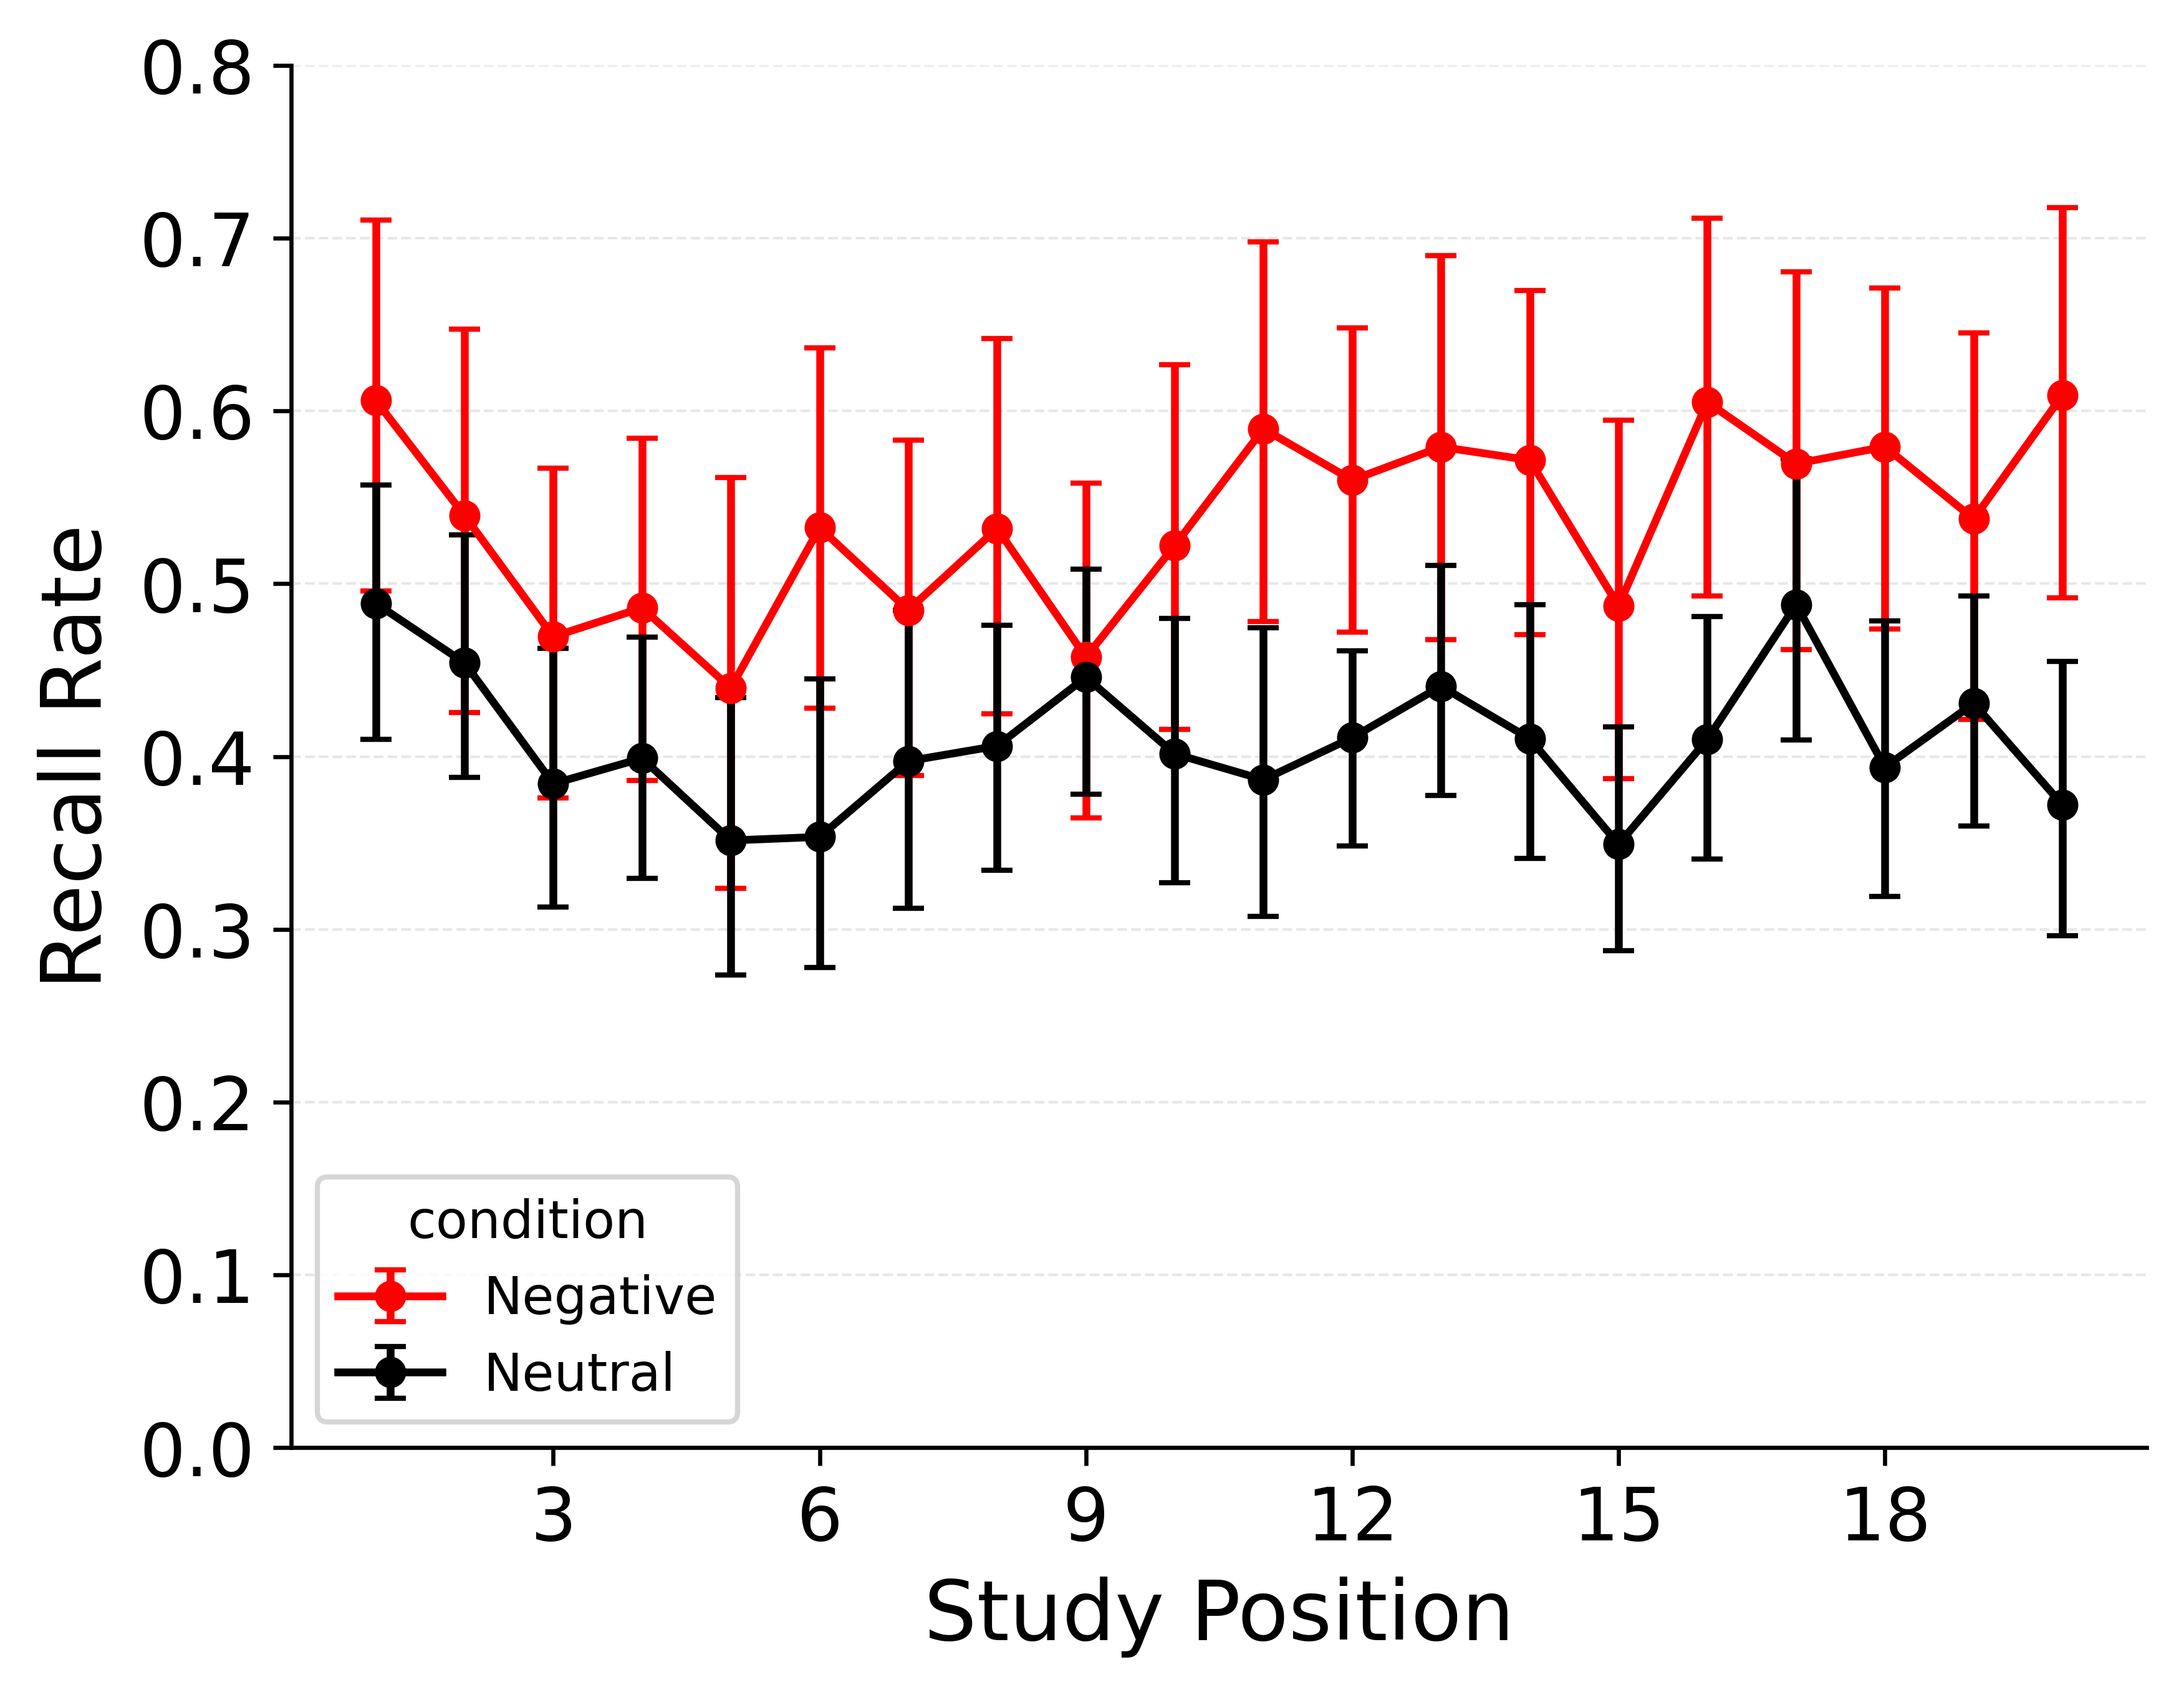
\includegraphics[keepaspectratio]{results/figures/analyses/reference_catspc.png}}\end{minipage}%
%
\begin{minipage}{0.50\linewidth}
\pandocbounded{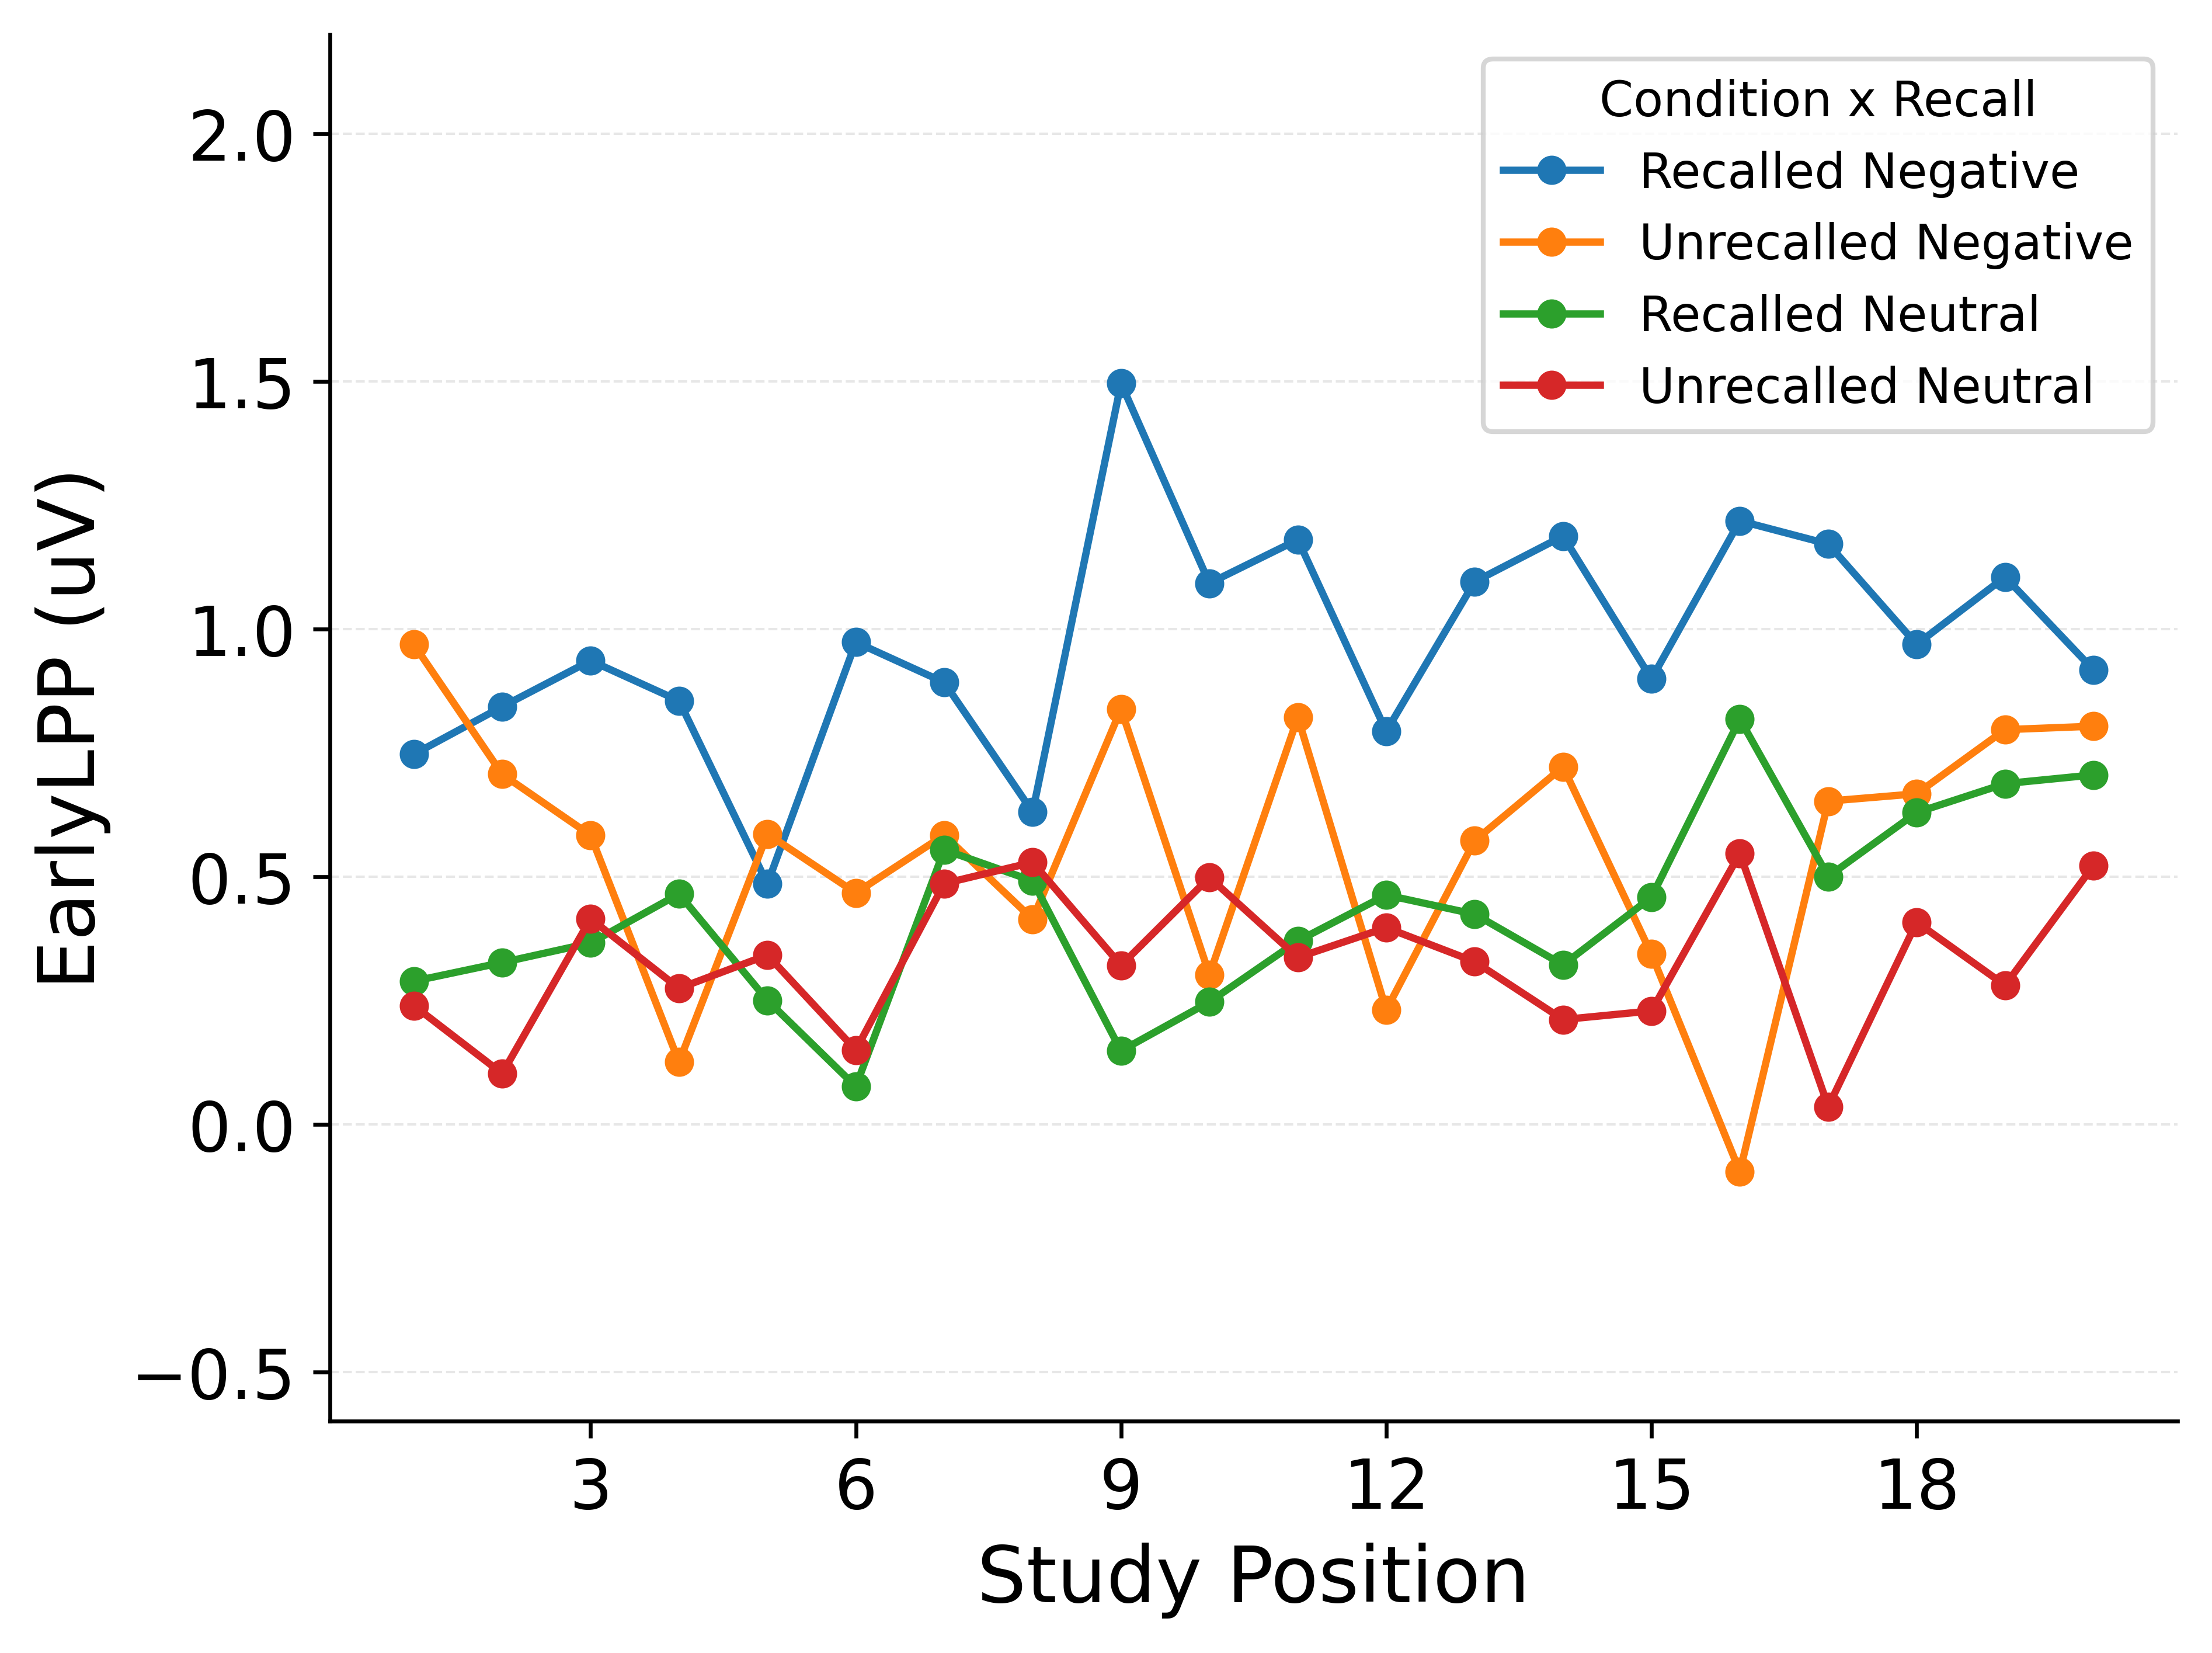
\includegraphics[keepaspectratio]{results/figures/cat_lpp_by_recall.png}}\end{minipage}%

\end{figure}%

\begin{figure}

\caption{\label{fig-eeg_emotion_only_fits}Simulated benchmarks for the
Emotion-only model. Left: Category-SPC from simulations using
per-subject fitted parameters, with negative (red) and neutral (black)
lines and bootstrapped 95\% CIs across subjects. Right: Early LPP by
recall status from the same simulations, with lines following the legend
labels (recalled/unrecalled negative and recalled/unrecalled neutral)
and CIs omitted.}

\begin{minipage}{0.50\linewidth}
\pandocbounded{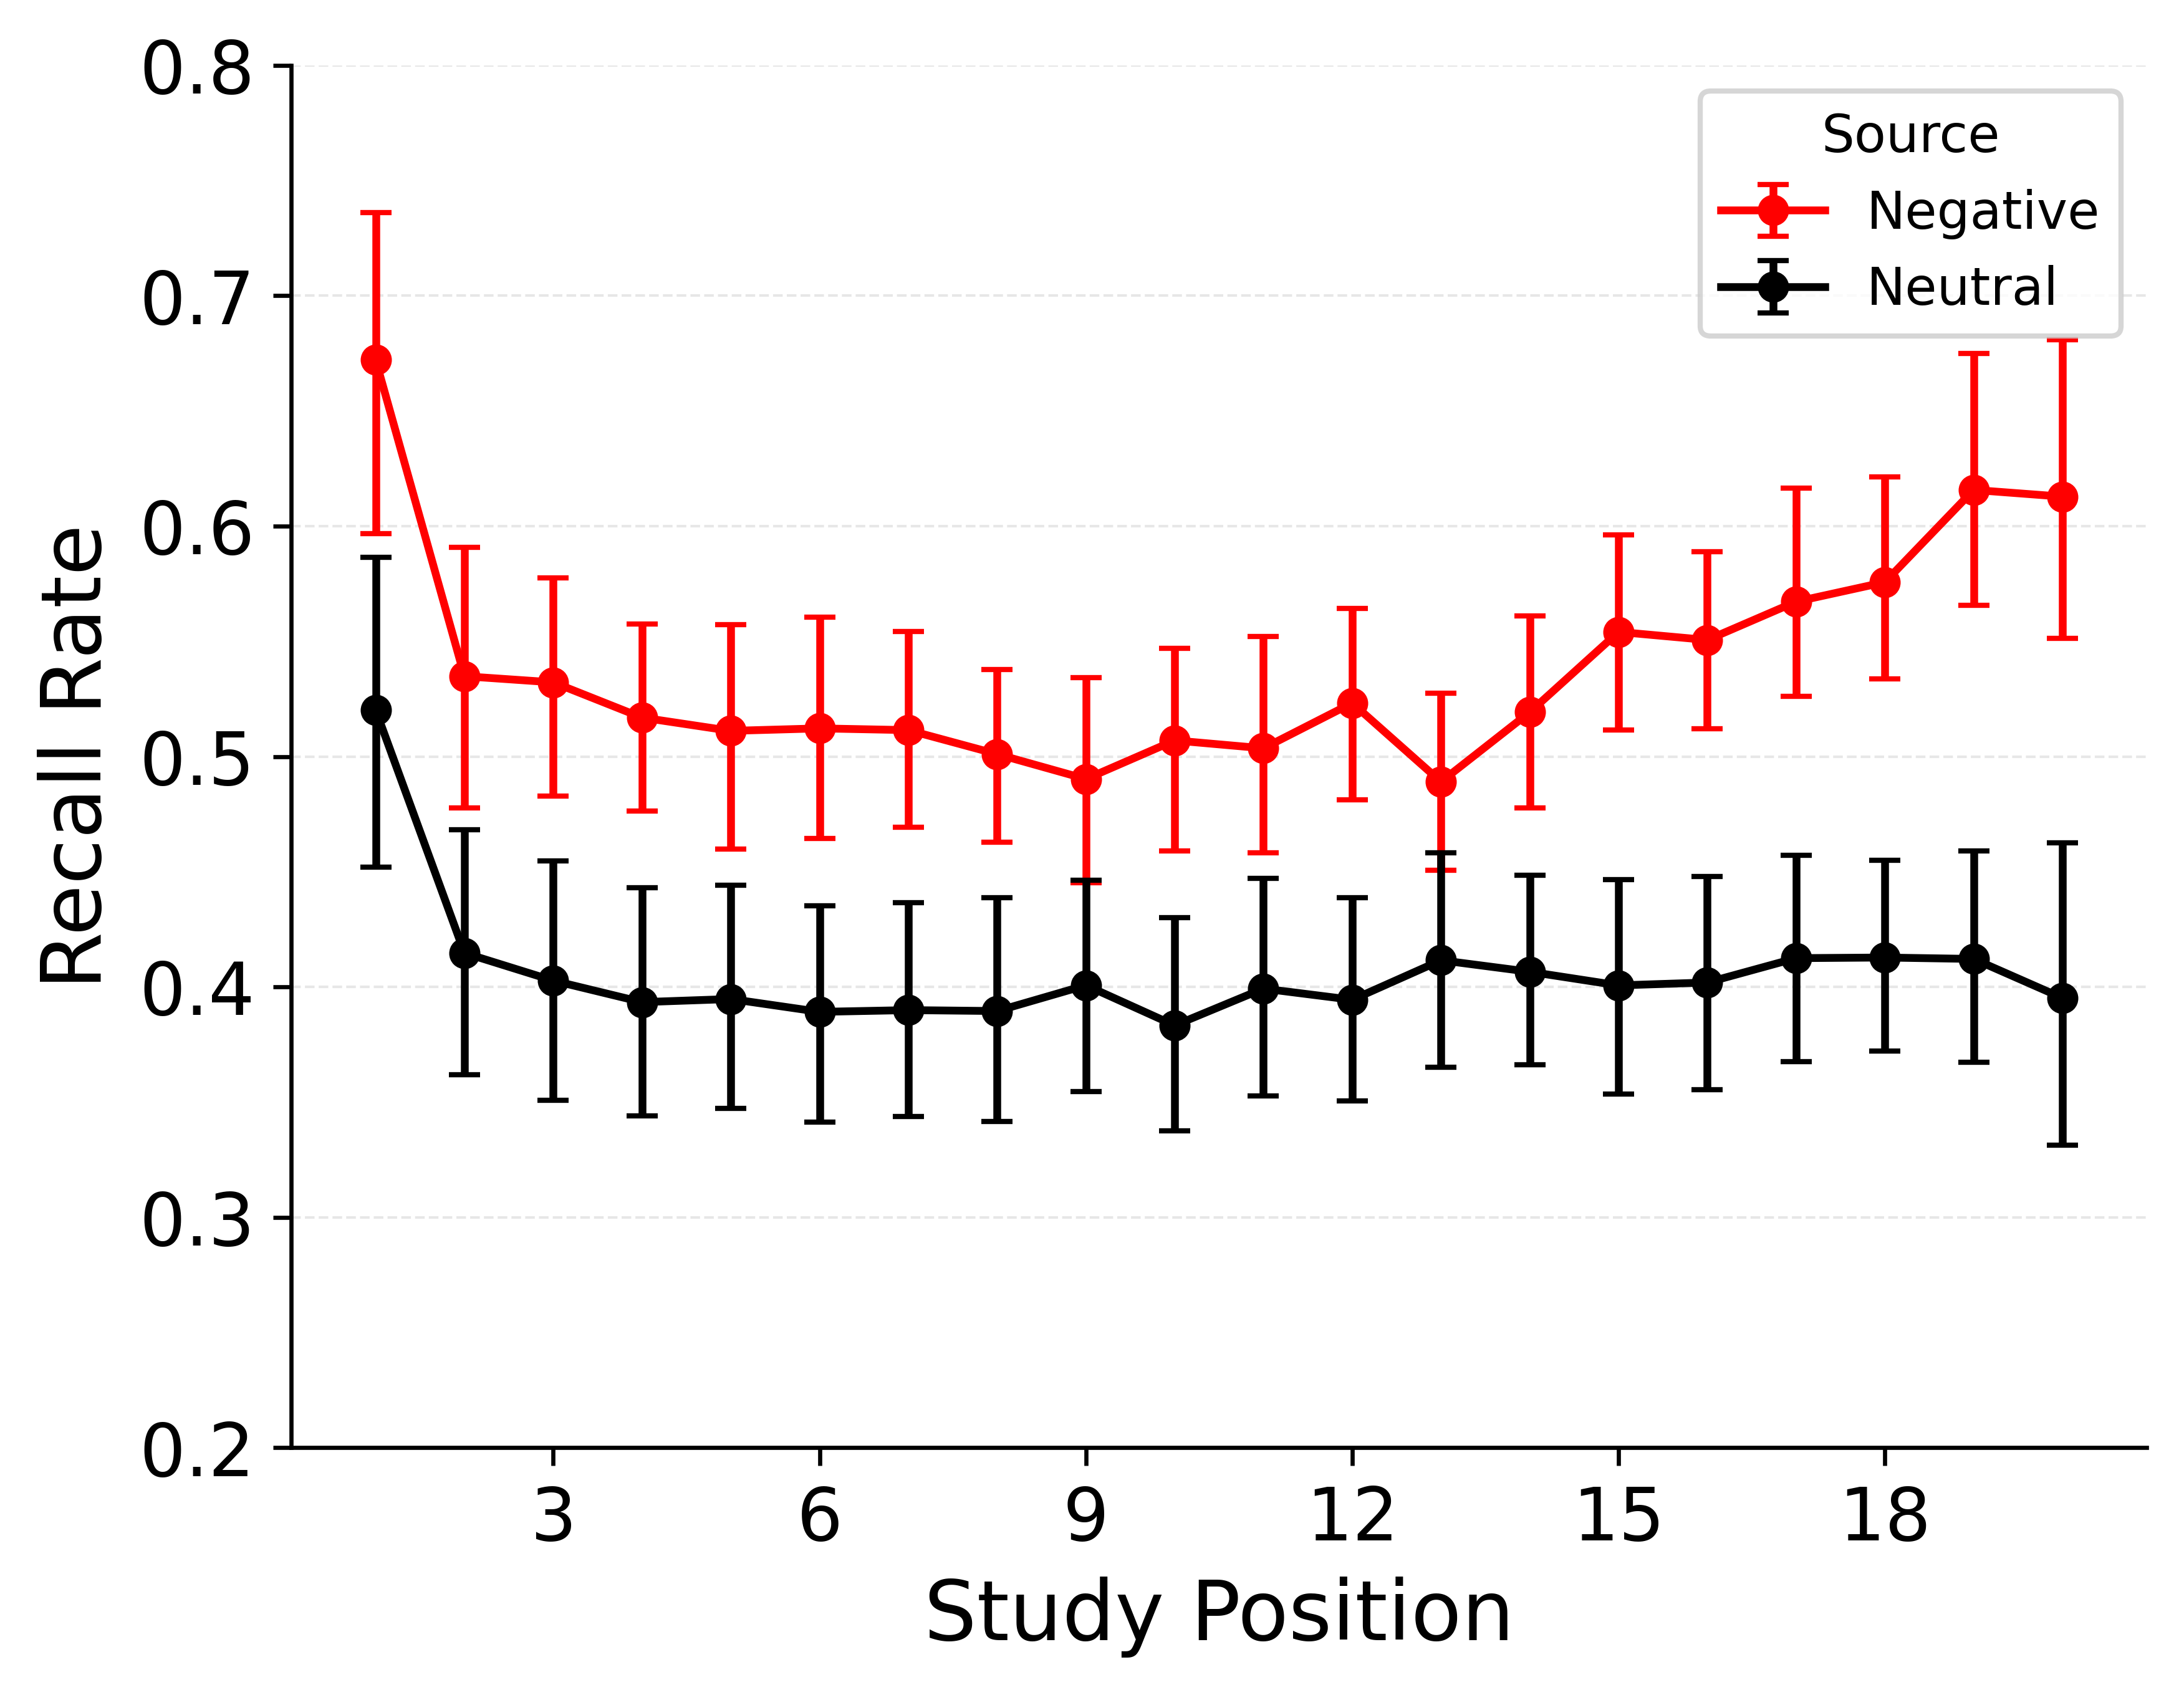
\includegraphics[keepaspectratio]{results/figures/fitting/TalmiEEG_EEGEmotionOnly_50_set_likelihood_fixed_term_best_of_3_cat_spc.png}}\end{minipage}%
%
\begin{minipage}{0.50\linewidth}
\pandocbounded{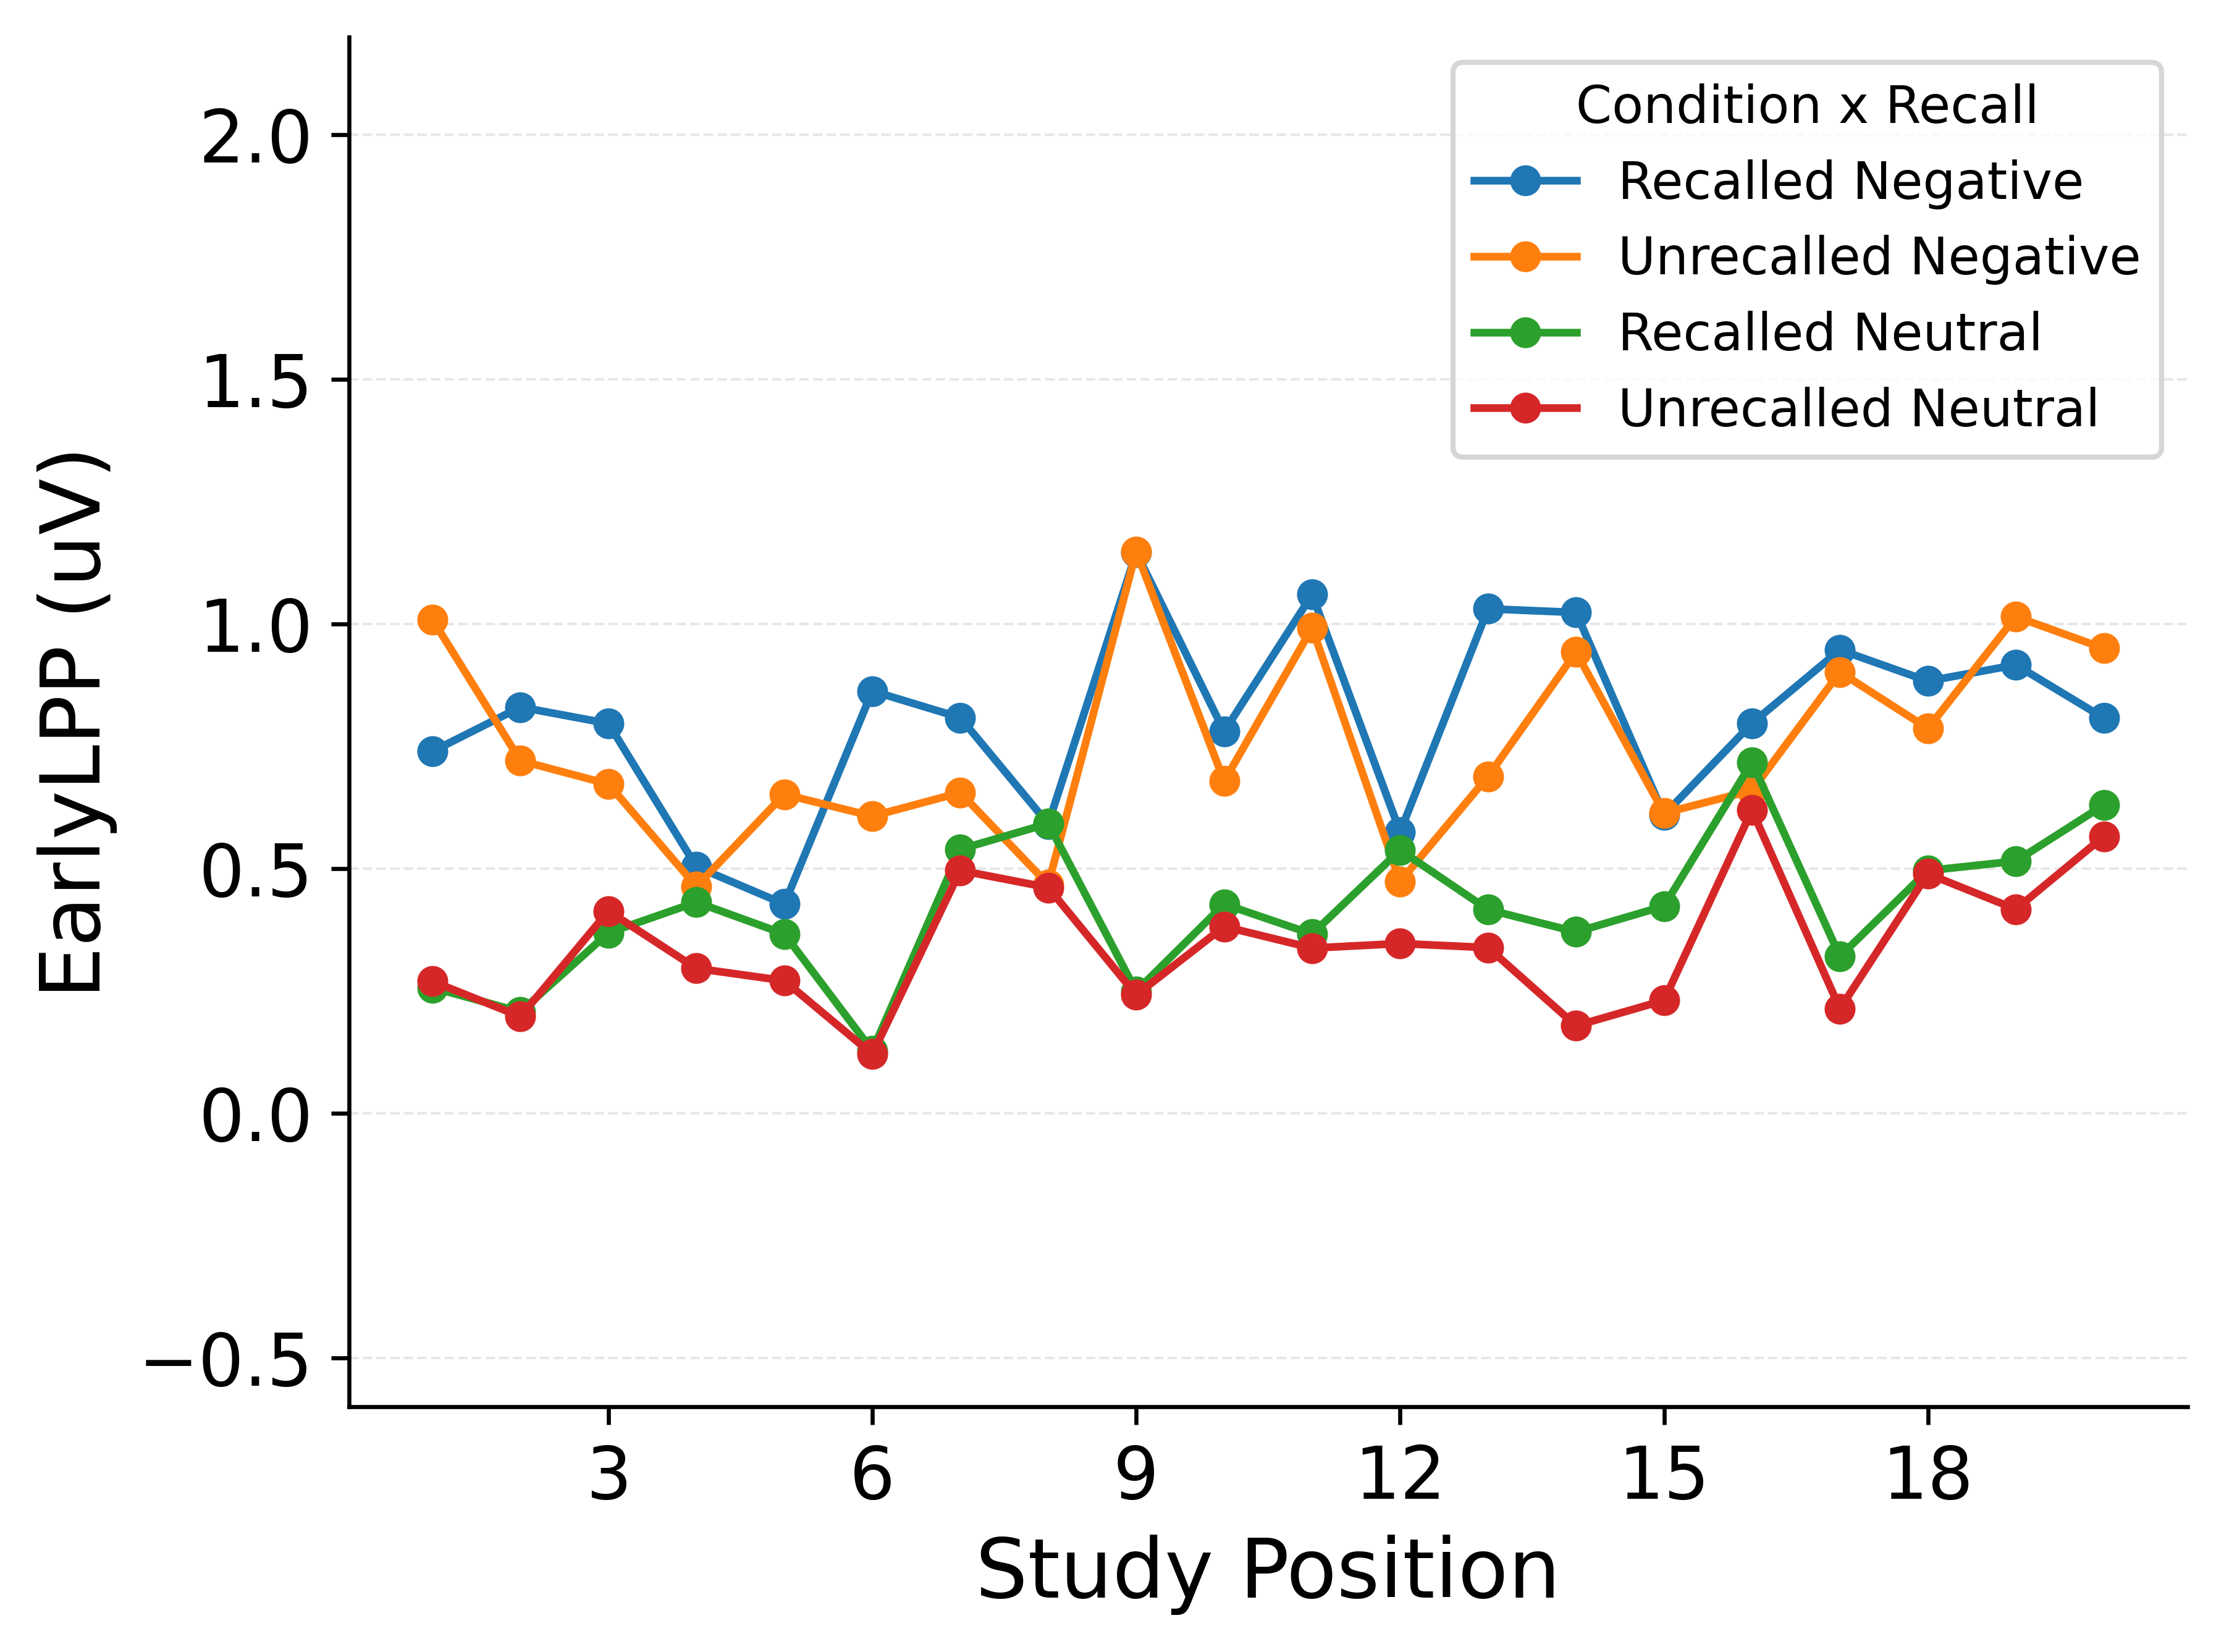
\includegraphics[keepaspectratio]{results/figures/fitting/TalmiEEG_EEGEmotionOnly_50_set_likelihood_fixed_term_best_of_3_cat_lpp_by_recall.png}}\end{minipage}%

\end{figure}%

\begin{figure}

\caption{\label{fig-eeg_main_effects_fits}Simulated benchmarks for the
Emotion + LPP (main effects) model. Left: Category-SPC from simulations
using per-subject fitted parameters, with negative (red) and neutral
(black) lines and bootstrapped 95\% CIs across subjects. Right: Early
LPP by recall status from the same simulations, with lines following the
legend labels (recalled/unrecalled negative and recalled/unrecalled
neutral) and CIs omitted.}

\begin{minipage}{0.50\linewidth}
\pandocbounded{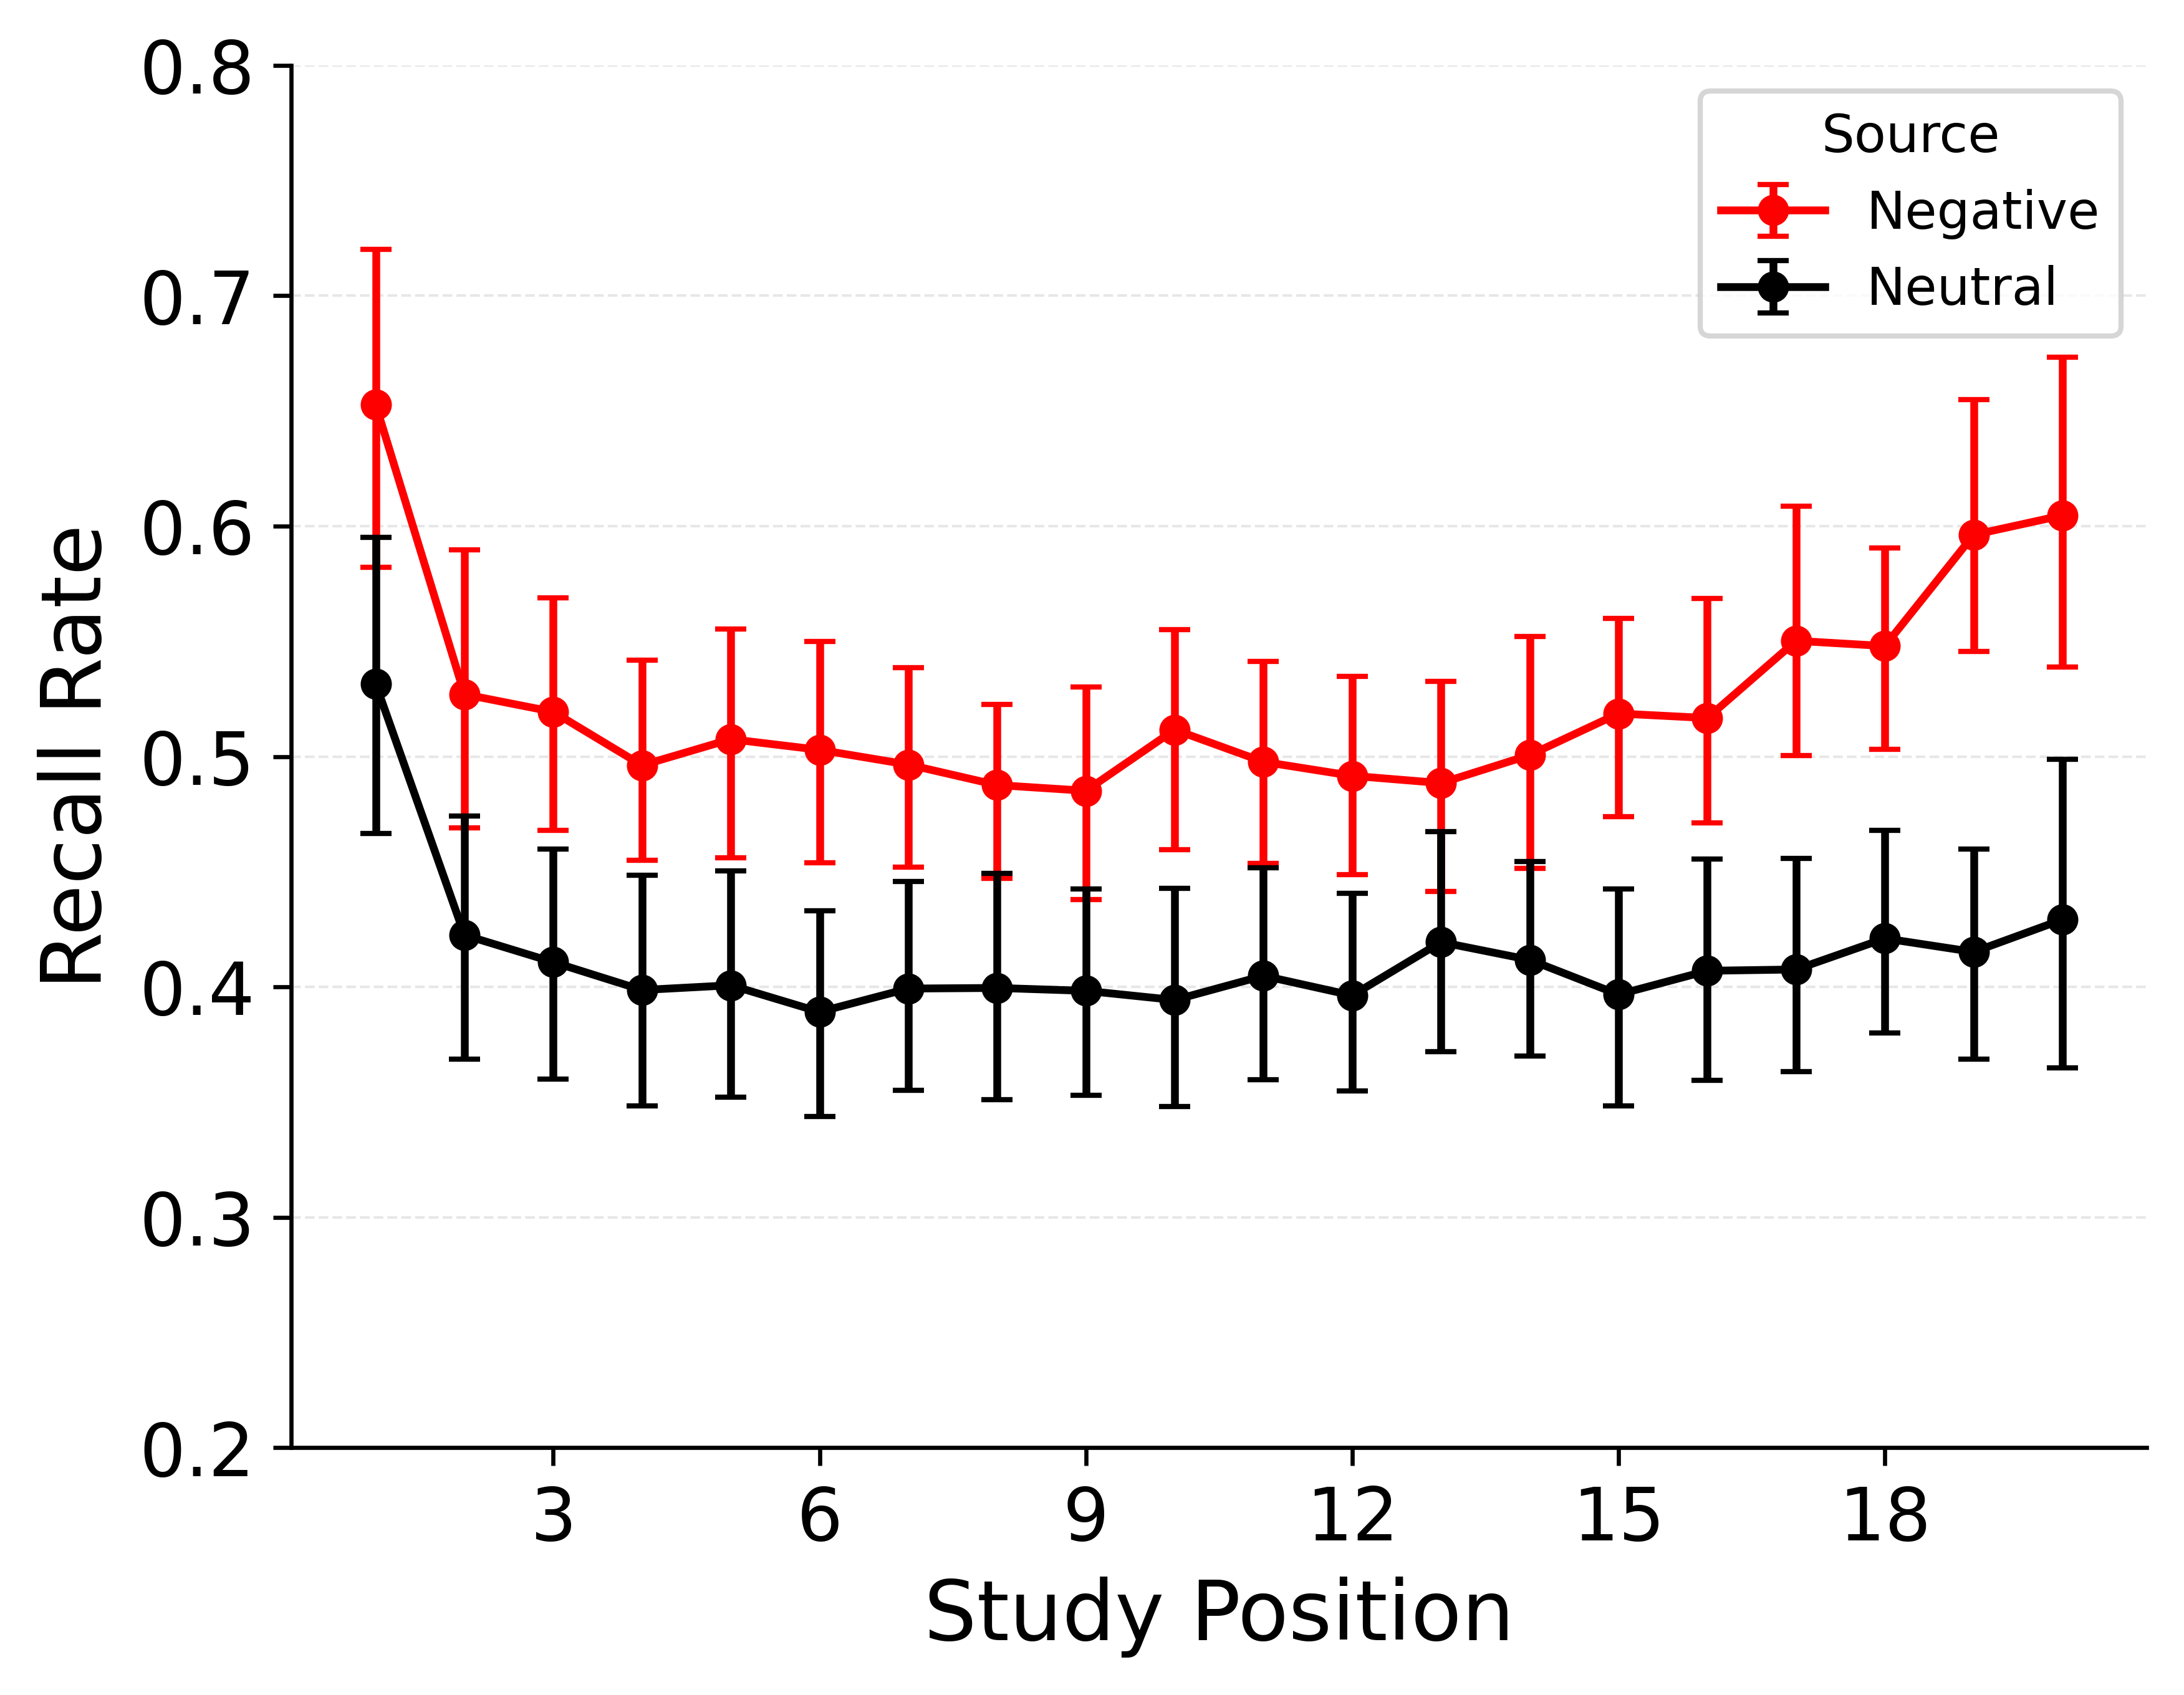
\includegraphics[keepaspectratio]{results/figures/fitting/TalmiEEG_EEGMainEffects_50_set_likelihood_fixed_term_best_of_3_cat_spc.png}}\end{minipage}%
%
\begin{minipage}{0.50\linewidth}
\pandocbounded{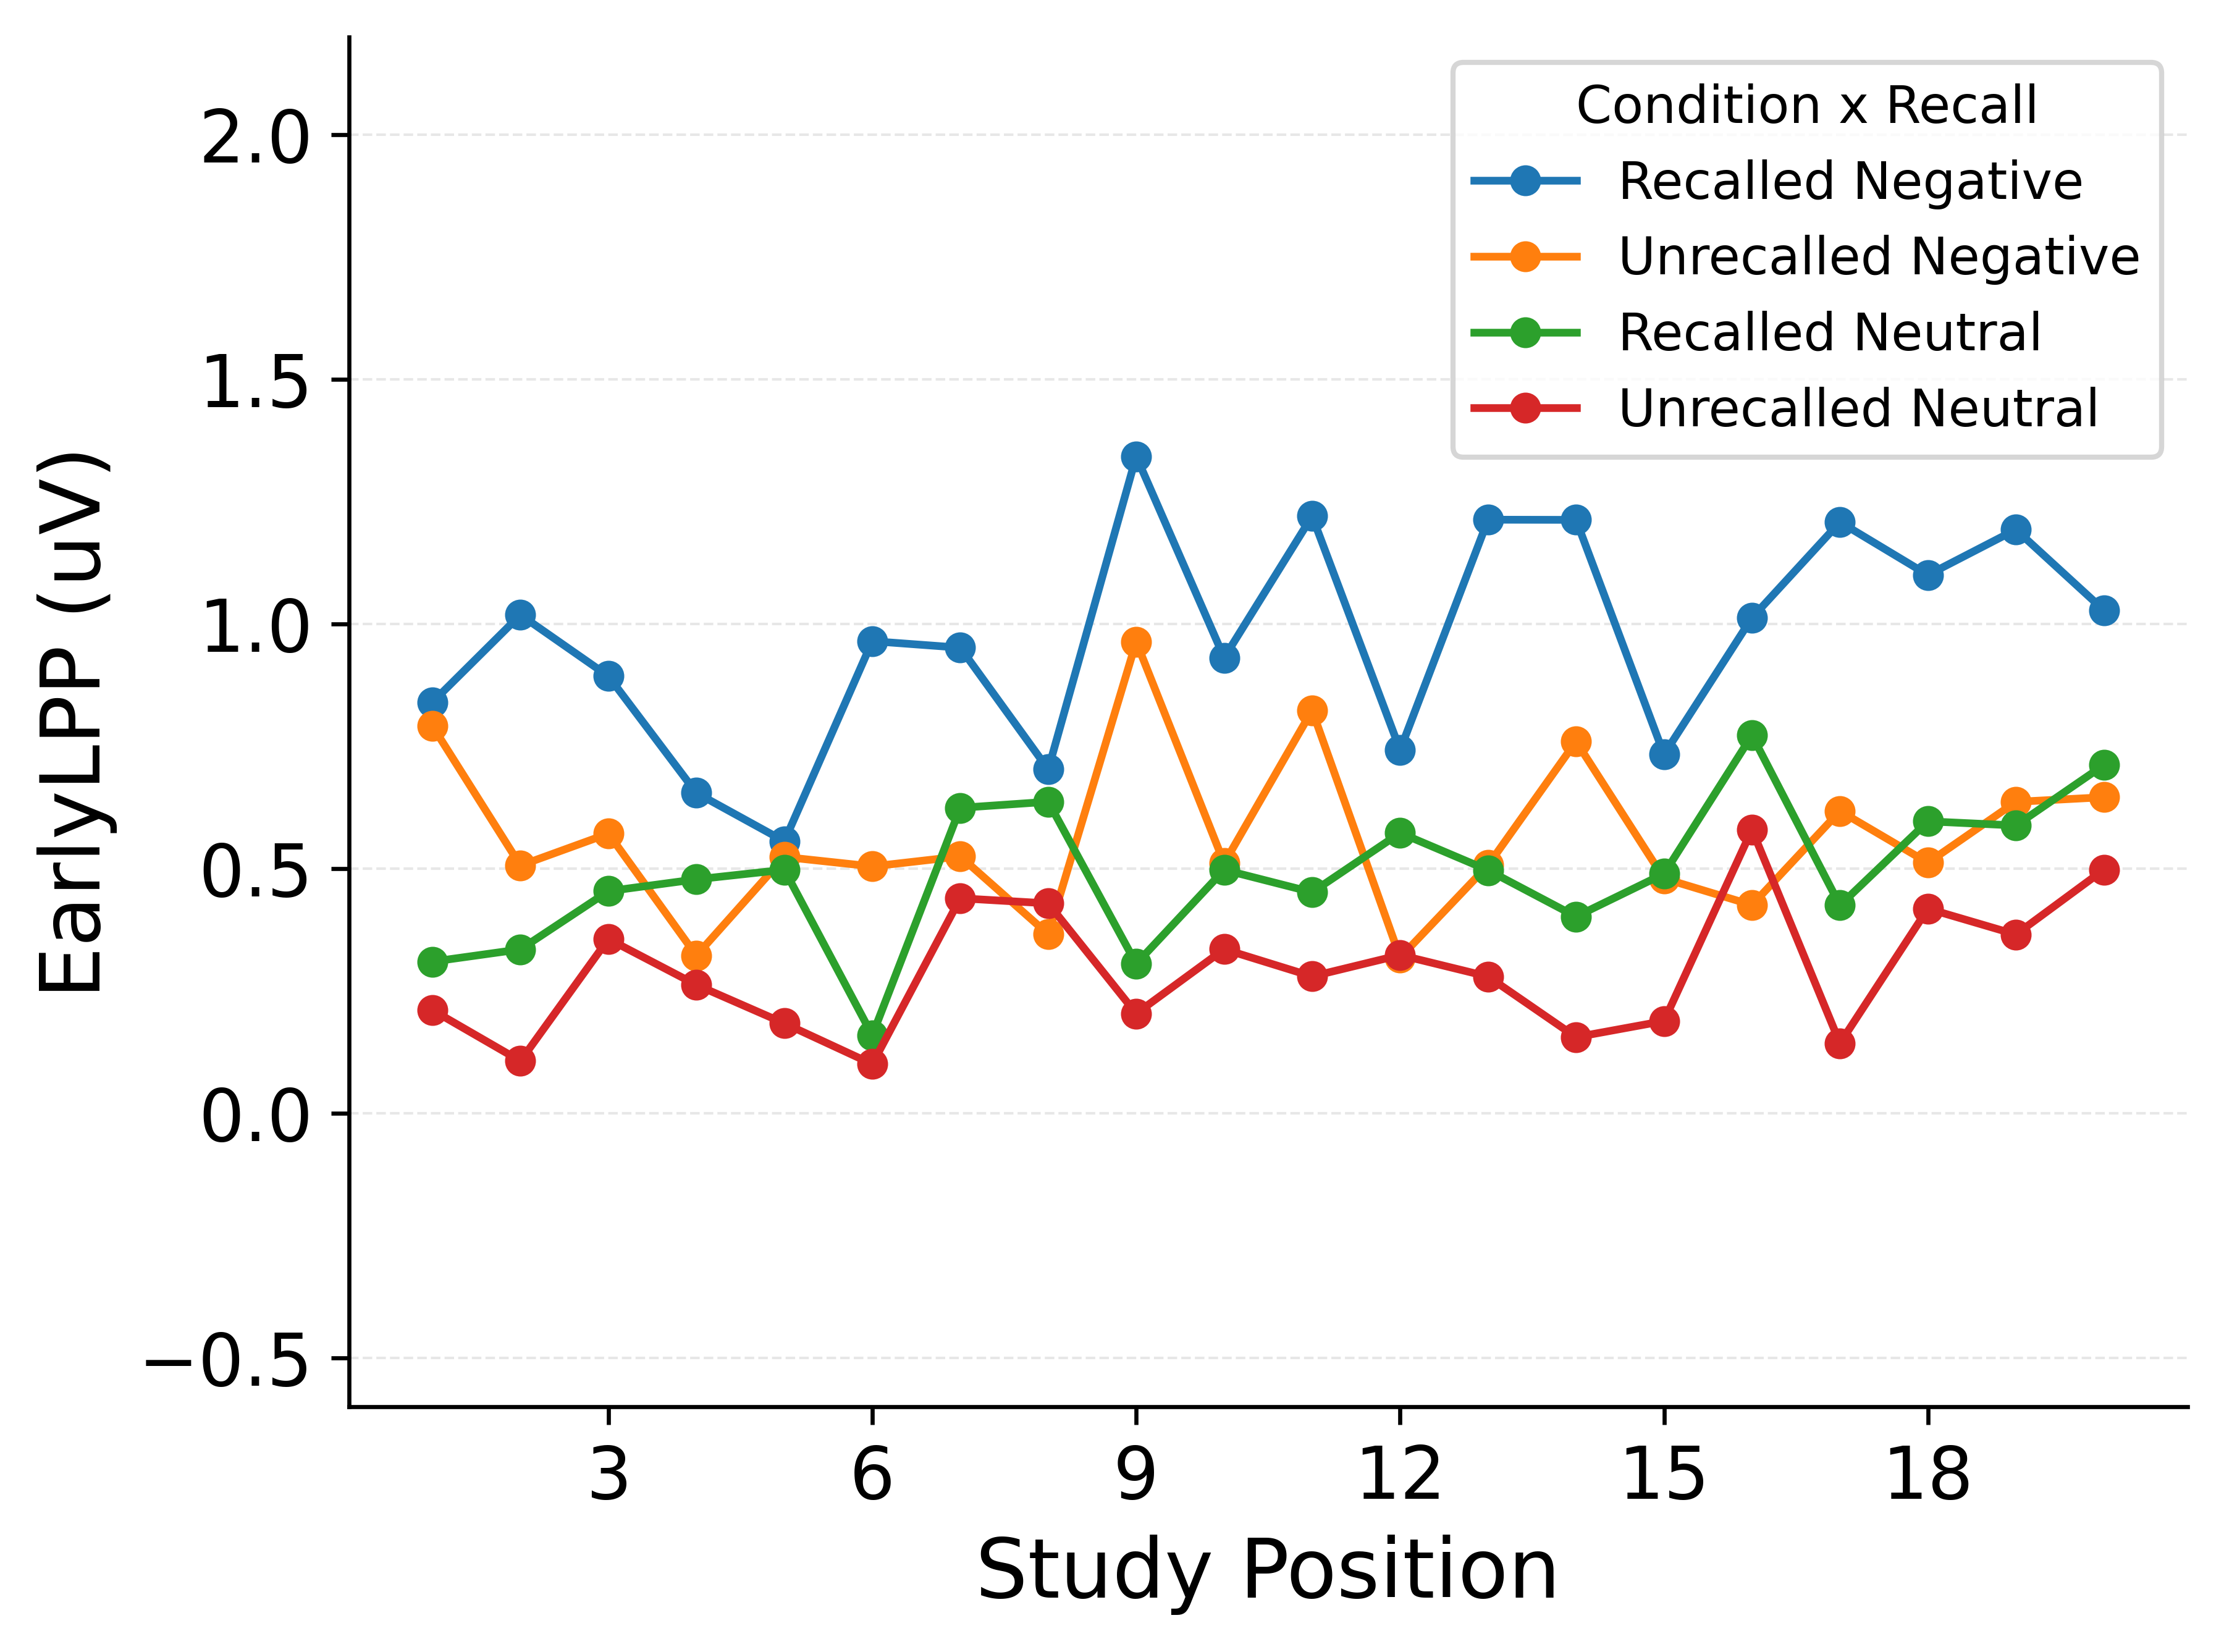
\includegraphics[keepaspectratio]{results/figures/fitting/TalmiEEG_EEGMainEffects_50_set_likelihood_fixed_term_best_of_3_cat_lpp_by_recall.png}}\end{minipage}%

\end{figure}%

\begin{figure}

\caption{\label{fig-eeg_main_effects_plus_interaction_fits}Simulated
benchmarks for the Emotion + LPP (interaction) model. Left: Category-SPC
from simulations using per-subject fitted parameters, with negative
(red) and neutral (black) lines and bootstrapped 95\% CIs across
subjects. Right: Early LPP by recall status from the same simulations,
with lines following the legend labels (recalled/unrecalled negative and
recalled/unrecalled neutral) and CIs omitted.}

\begin{minipage}{0.50\linewidth}
\pandocbounded{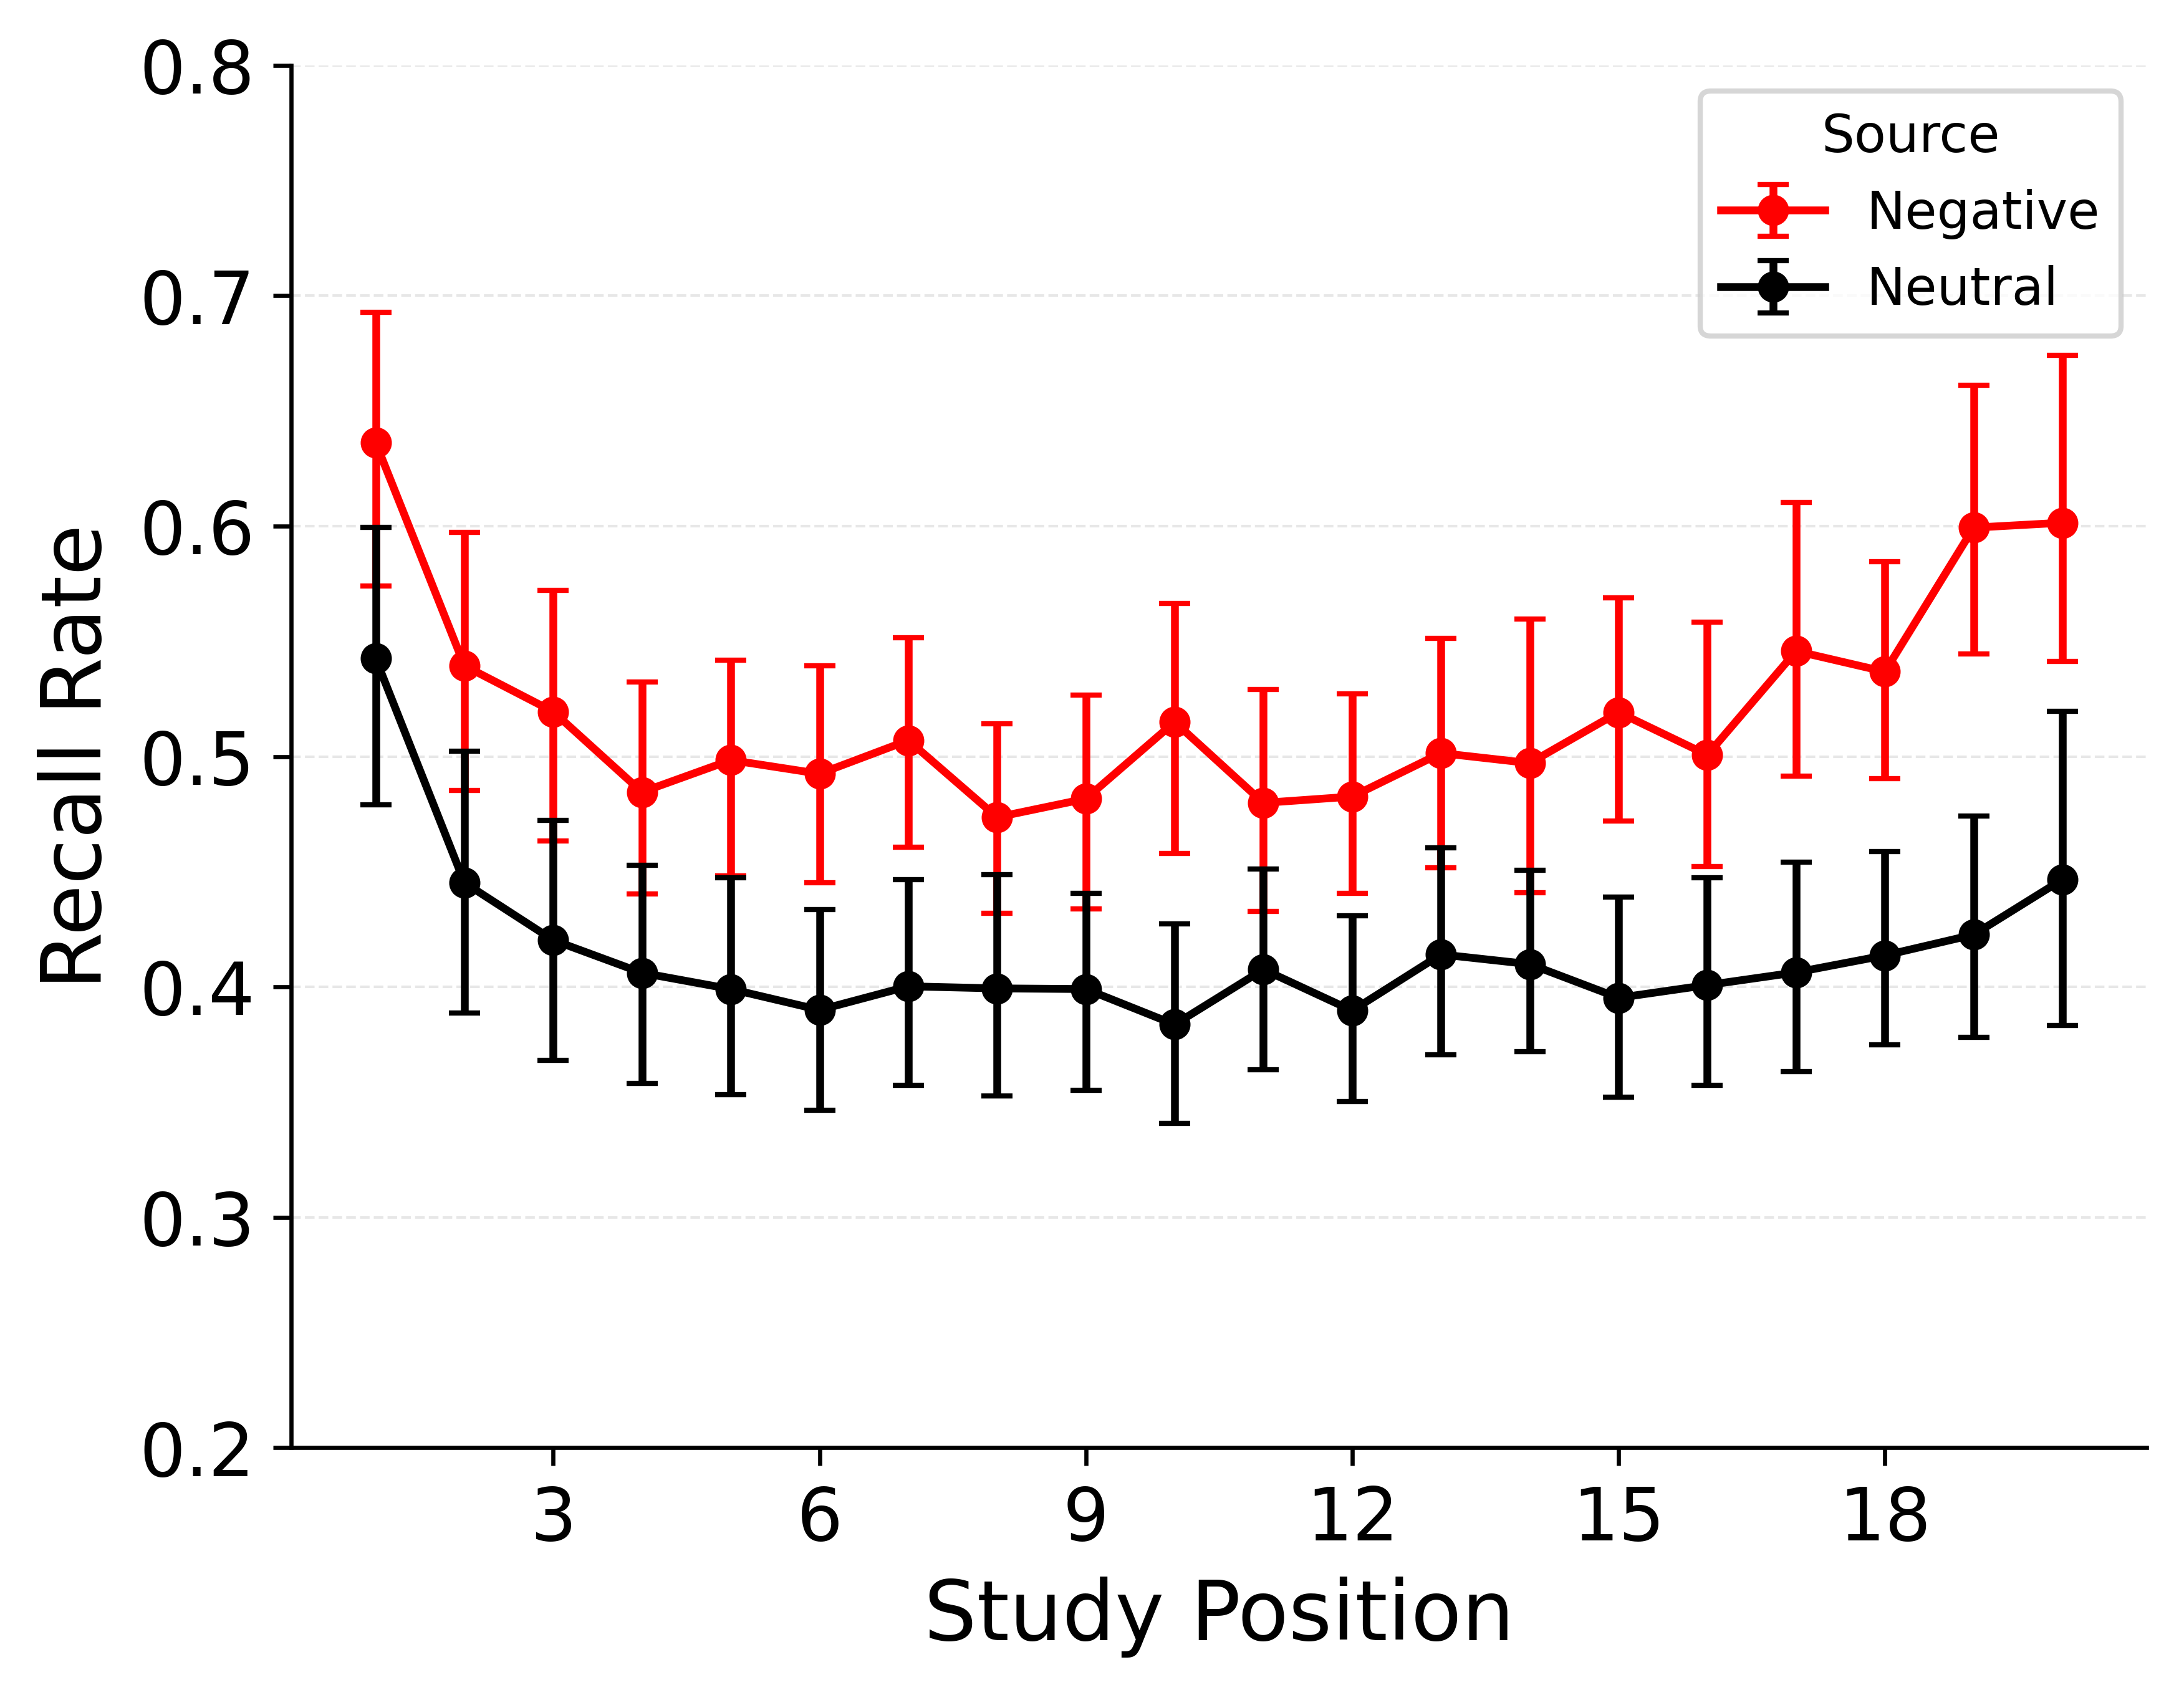
\includegraphics[keepaspectratio]{results/figures/fitting/TalmiEEG_EEGMainEffectsPlusInteraction_50_set_likelihood_fixed_term_best_of_3_cat_spc.png}}\end{minipage}%
%
\begin{minipage}{0.50\linewidth}
\pandocbounded{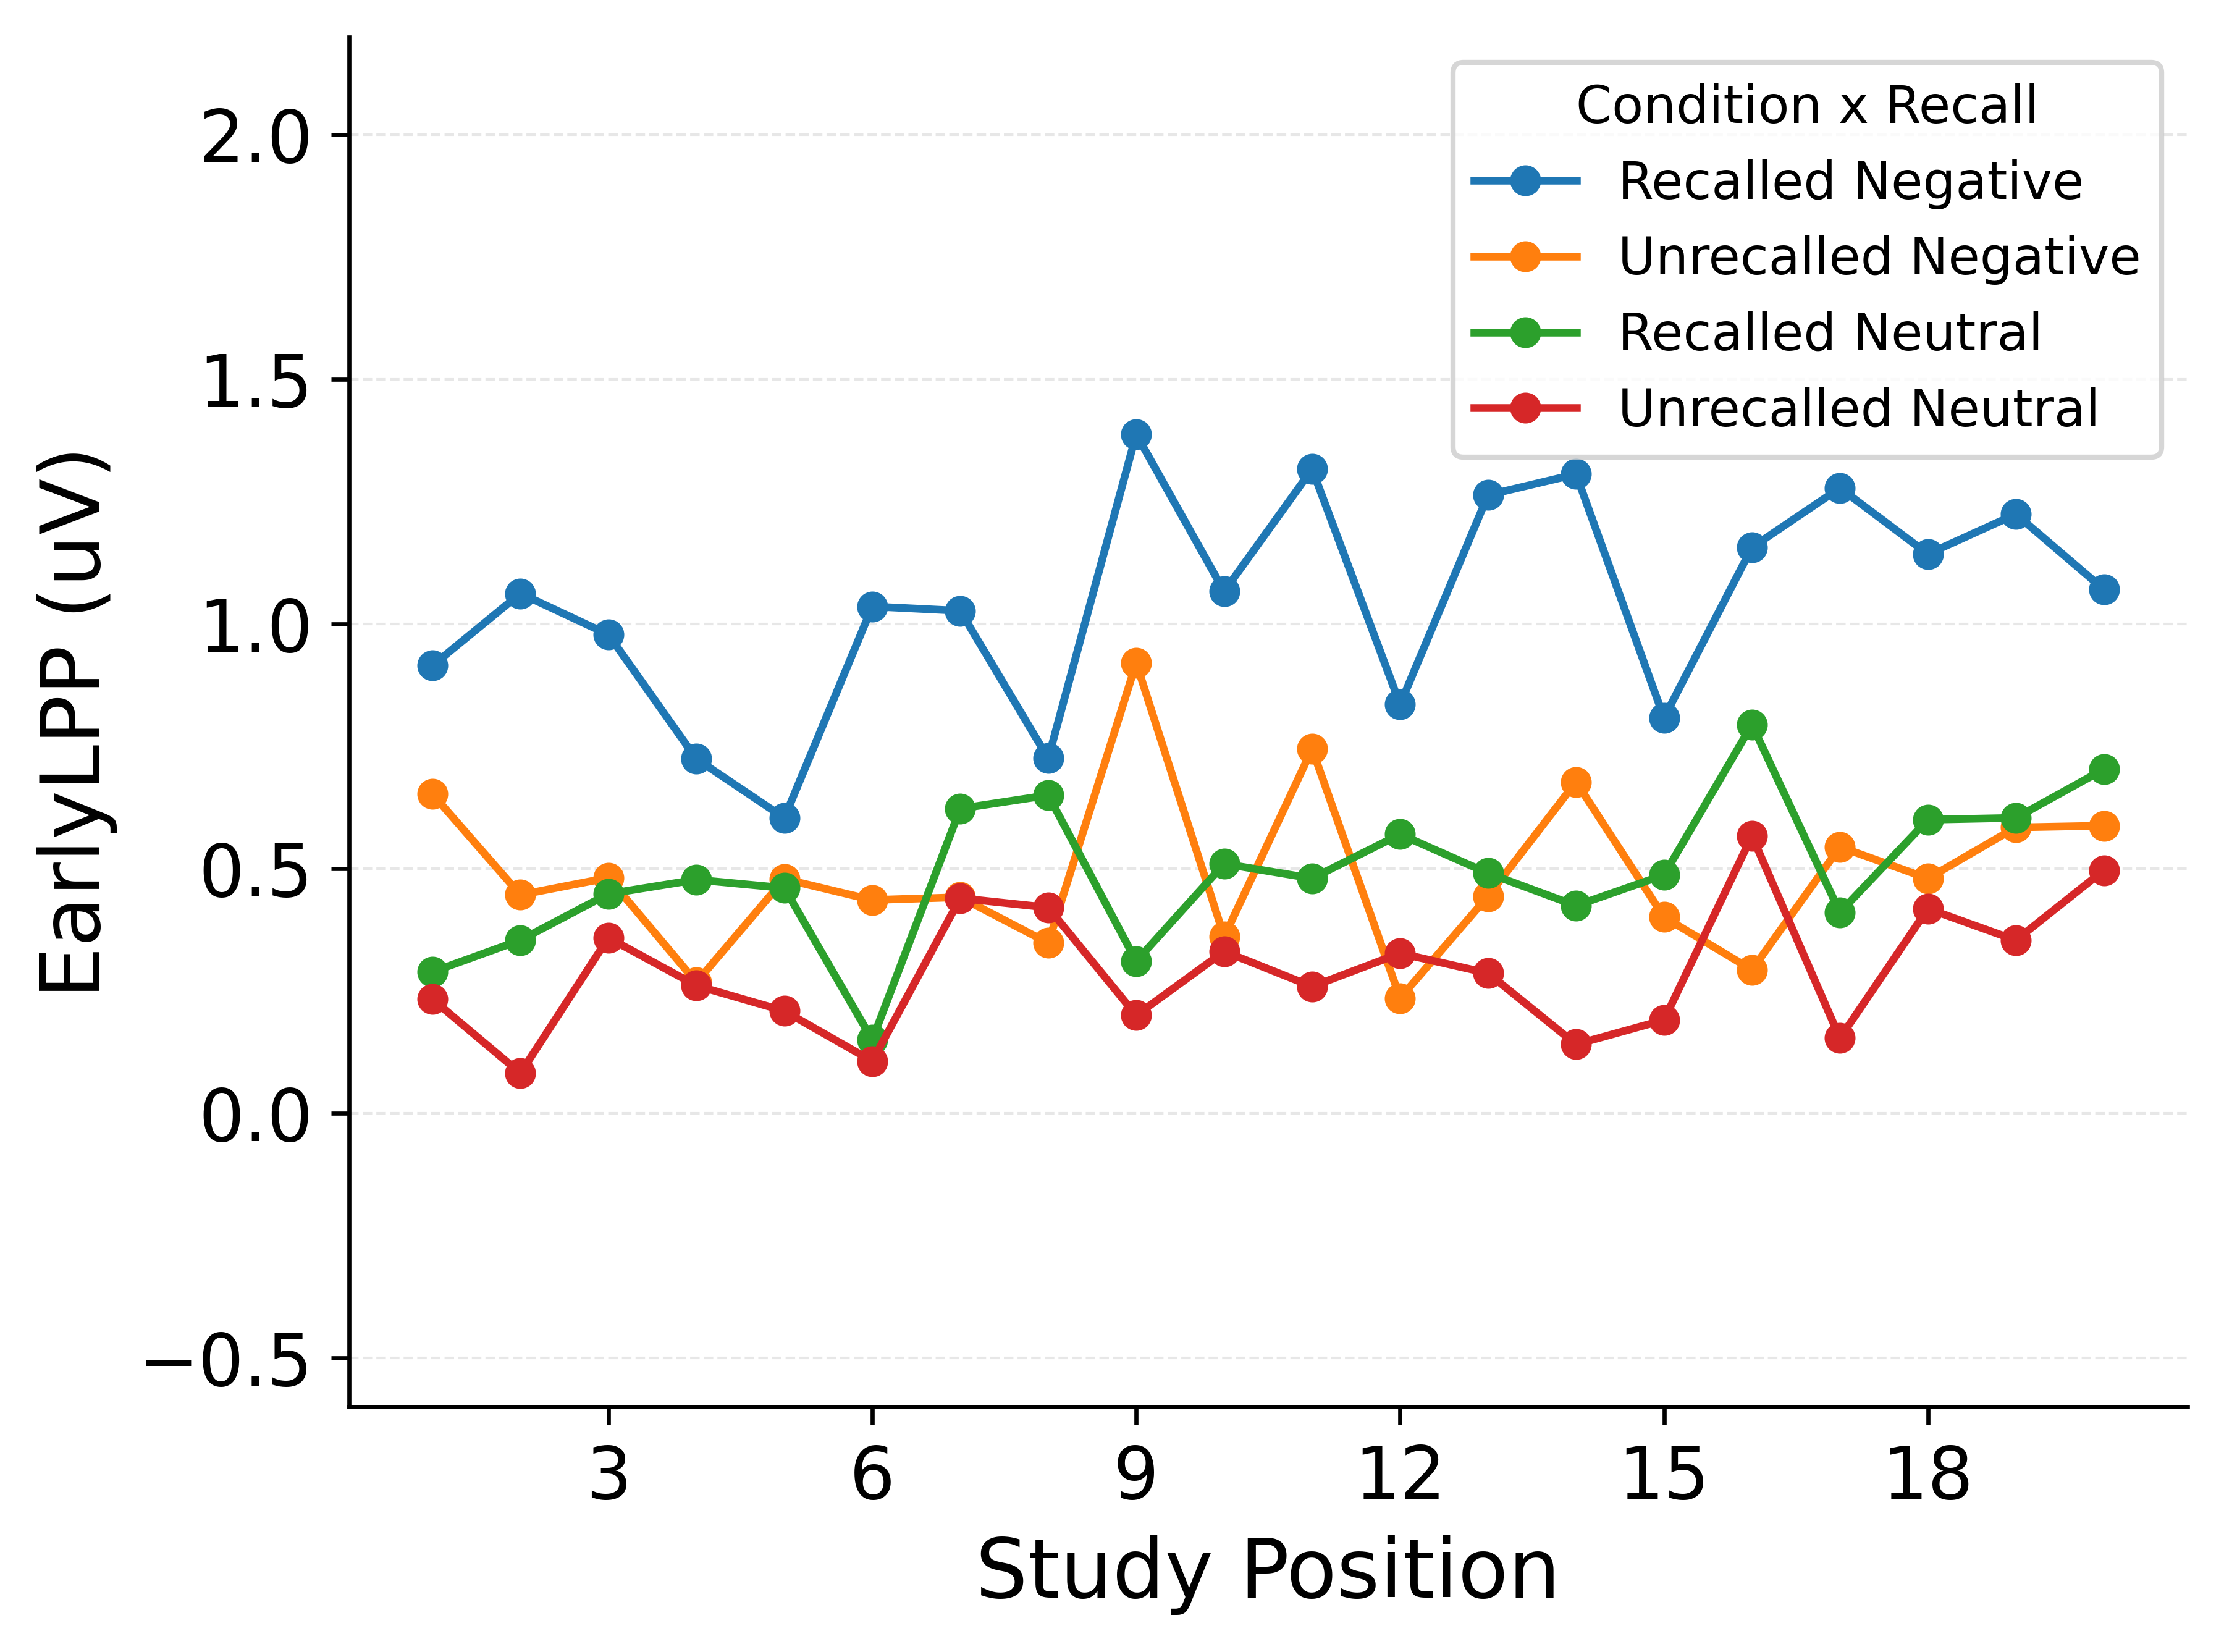
\includegraphics[keepaspectratio]{results/figures/fitting/TalmiEEG_EEGMainEffectsPlusInteraction_50_set_likelihood_fixed_term_best_of_3_cat_lpp_by_recall.png}}\end{minipage}%

\end{figure}%

In the Emotion-only simulations, the model captures much of the
emotional enhancement of memory in the Category-SPC but shows little
separation between recalled and unrecalled negative items in Early LPP.
This pattern indicates that emotion labels alone can reproduce the
overall category advantage without explaining LPP-linked recall
differences. In the Emotion + LPP (main effects) simulations, the model
fits both summary statistics but assigns a larger recalled--unrecalled
difference for neutral items and a smaller difference for negative
items. This pattern suggests that a single LPP slope captures the
overall association while misallocating the emotion-specific separation.
In the Emotion + LPP (interaction) simulations, the Category-SPC
preserves emotional enhancement of memory and the Early LPP panel shows
a clearer emotion-dependent separation between recalled and unrecalled
items. Together these benchmarks indicate that combining emotion and LPP
with an interaction provides the most faithful account of both the
category-level advantage and the emotion-specific LPP--recall pattern.

\appendix

\subsection{LPP by Item Type and Recall
Status}\label{lpp-by-item-type-and-recall-status}

\begin{figure}

\caption{\label{fig-amplitude_by_cat_by_recalled}LPP by time, recall
status, and item type.}

\centering{

\pandocbounded{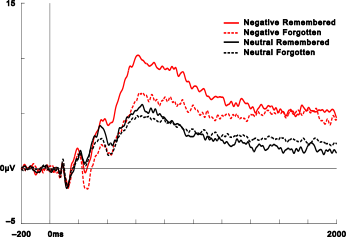
\includegraphics[keepaspectratio]{results/figures/amplitude_by_cat_by_recalled.png}}

}

\end{figure}%

\subsection{Recall Rate by Early LPP}\label{recall-rate-by-early-lpp}

This analysis is deprecated. It binned items by LPP amplitude within
item category and plotted recall rates per bin to check whether LPP
predicts recall beyond the emotional/neutral label. Bins were defined by
percentiles of the pooled LPP distribution, and results were shown
separately for Early LPP (400--700\,ms) and Late LPP (700--1,000\,ms).
LPP values were the provided z‑normalized amplitudes computed per
electrode and trial by subtracting the −200--0\,ms baseline and dividing
by the baseline SD (so values are on a mean‑0, SD‑1 scale). An earlier
plotting bug set a participant's bin value to zero when they contributed
no items to that bin, which biased sparse bins downward; this has been
fixed by excluding empty participant--bin cells from the proportion and
confidence‑interval calculations. The reference figure displays lines
predicted by a generalized mixed‑effects model of recall as a function
of LPP and item category, whereas the current plot shows empirical
proportions within bins; the two approaches diverge most at distribution
tails where data are sparse.

As seen in Figure~\ref{fig-cat_recall_by_early_lpp}, recall rates rise
with Early LPP for emotional items and are comparatively flatter for
neutral items. Observations were distributed unevenly across bins (see
count panels in Figure~\ref{fig-cat_recall_by_lpp_counts}). Because
there are more neutral than emotional items overall, neutral items
appear more frequently in every LPP bin. However, since recall rates are
proportions within bin, this does not bias the curves. Still, wide
intervals at extreme LPP values reflect very low occupancy in those bins
(and thus high uncertainty about recall rates there).

\begin{figure}

\caption{\label{fig-cat_recall_by_early_lpp}Recall rate by Early LPP
amplitude and item type in reference materials (LEFT) and in the present
dataset (RIGHT).}

\begin{minipage}{0.50\linewidth}
\pandocbounded{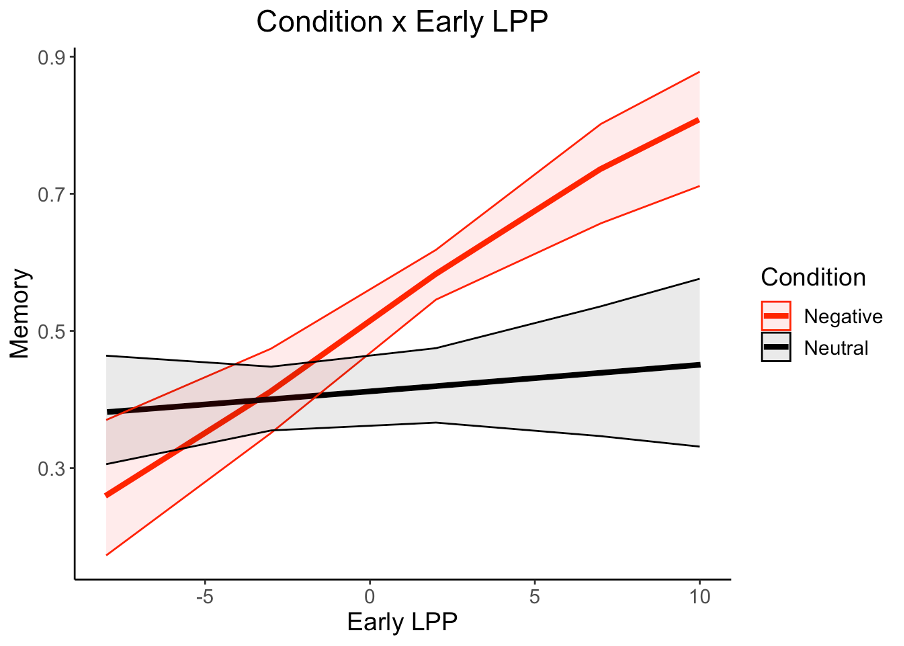
\includegraphics[keepaspectratio]{results/figures/reference_cat_recall_by_lpp.png}}\end{minipage}%
%
\begin{minipage}{0.50\linewidth}
\pandocbounded{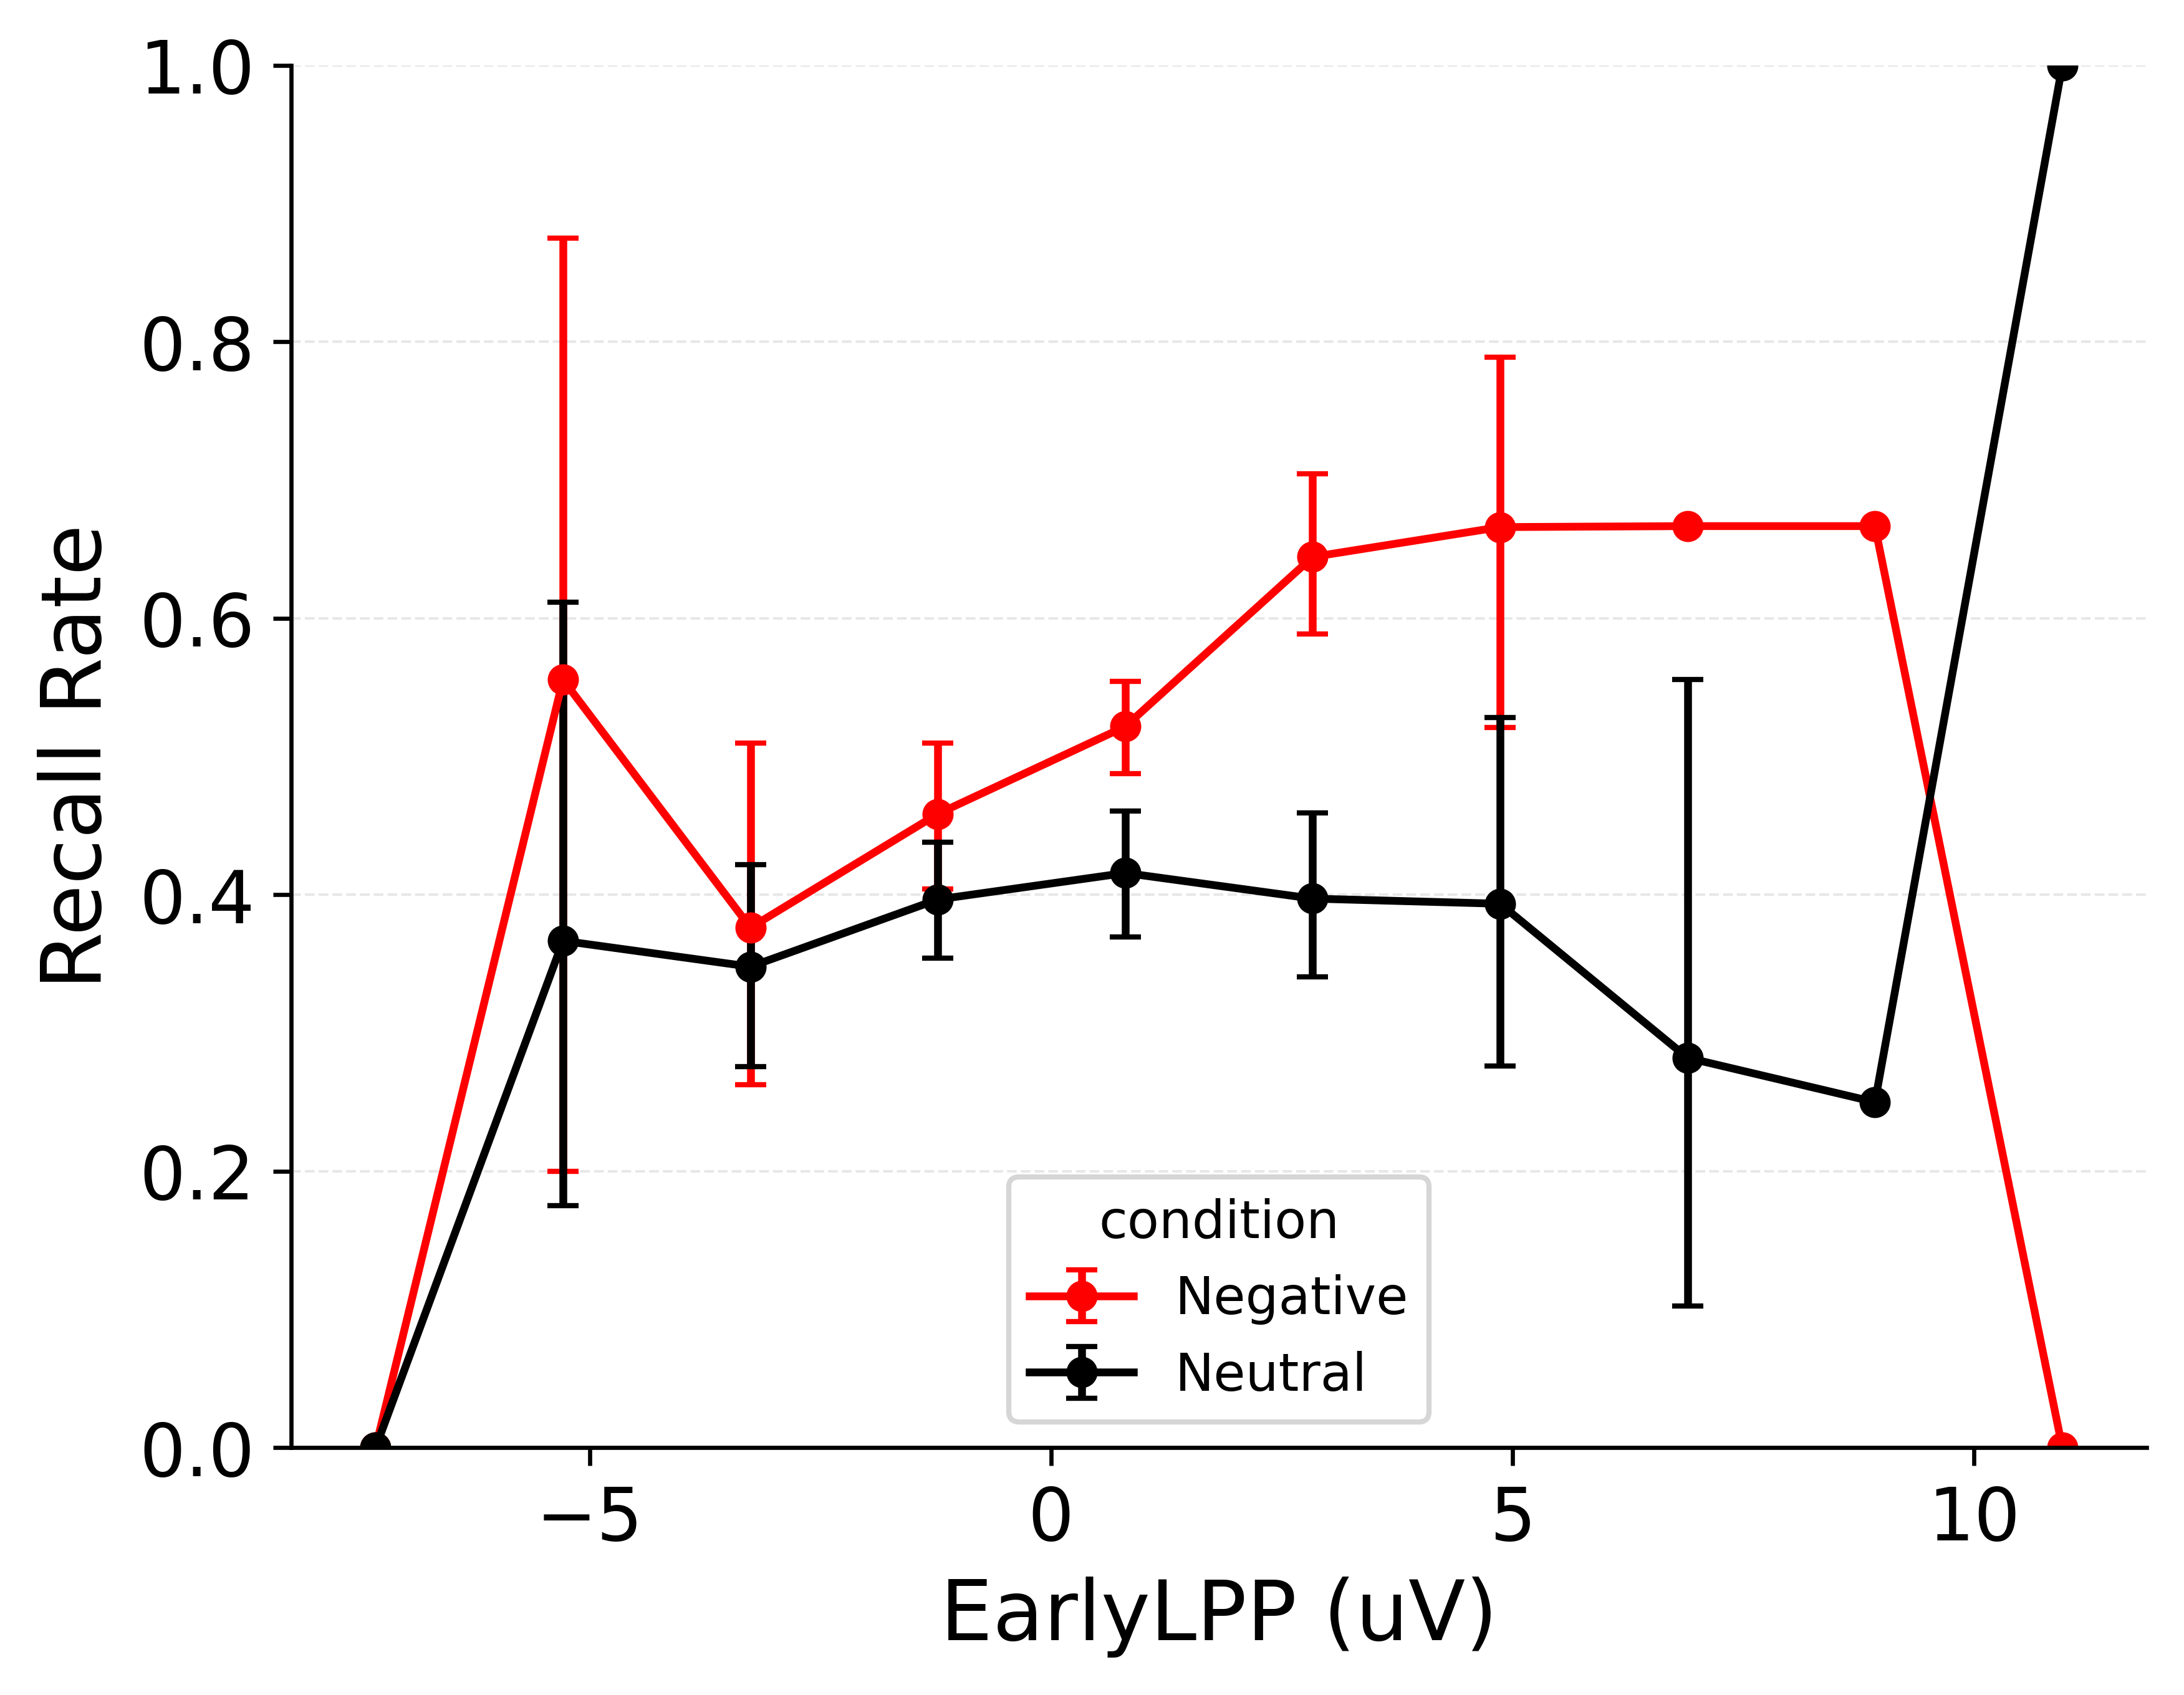
\includegraphics[keepaspectratio]{results/figures/analyses/cat_recall_by_lpp_EarlyLPP.png}}\end{minipage}%

\end{figure}%

We deprecate this analysis because binning introduces instability and
comparability problems: tail bins above roughly 4.86 and below −3.25
contain few observations, global percentile bins balance totals but not
per‑category counts, and bin‑edge choices can change the apparent trend
without changing the underlying data. Rather than redefine or stabilize
the binning procedure, we opt to retire it. For inference and model
development we instead rely on unbinned methods (generalized
mixed‑effects models and likelihood‑based evaluation of full recalled
sets) and on visualizations that condition on recall status without
binning (e.g., Figure~\ref{fig-cat_lpp_by_recall_split}). The plots are
retained only as qualitative checks against the reference analysis.

\begin{figure}

\caption{\label{fig-cat_recall_by_lpp_counts}Counts of observations per
bin for Early LPP (LEFT) and Late LPP (RIGHT).}

\begin{minipage}{0.50\linewidth}
\pandocbounded{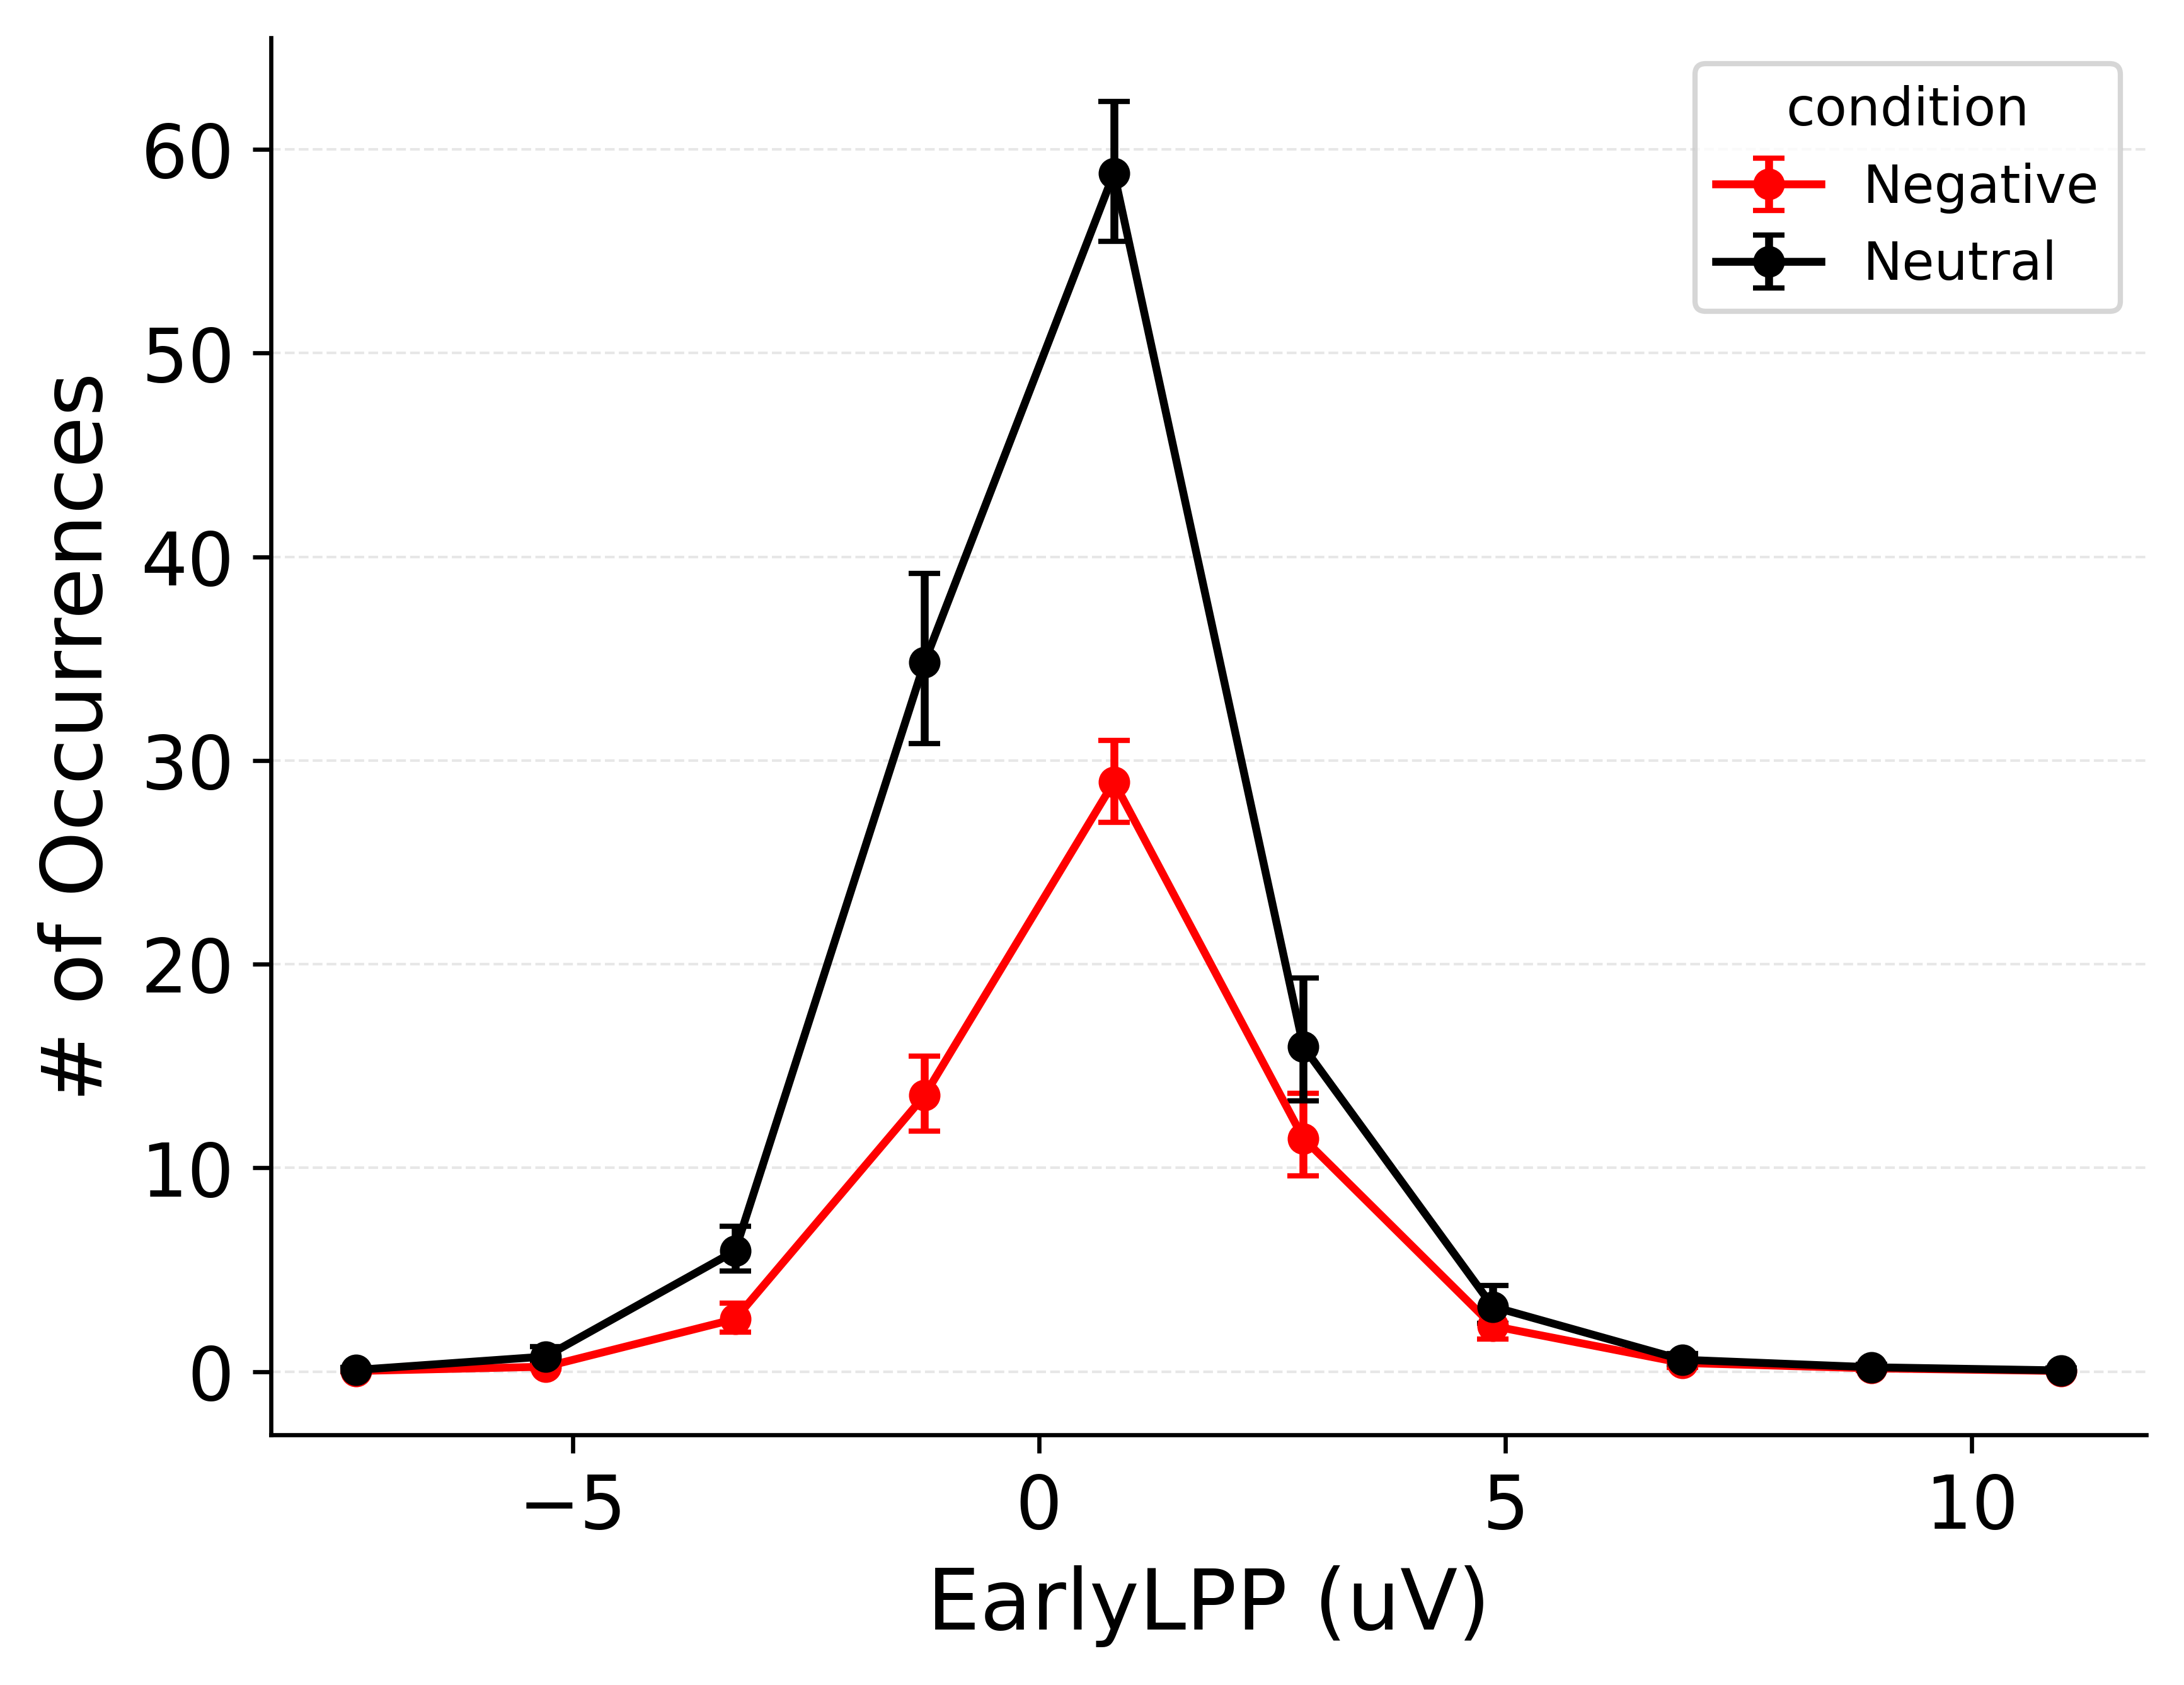
\includegraphics[keepaspectratio]{results/figures/analyses/cat_recall_by_lpp_EarlyLPP_counts.png}}\end{minipage}%
%
\begin{minipage}{0.50\linewidth}
\pandocbounded{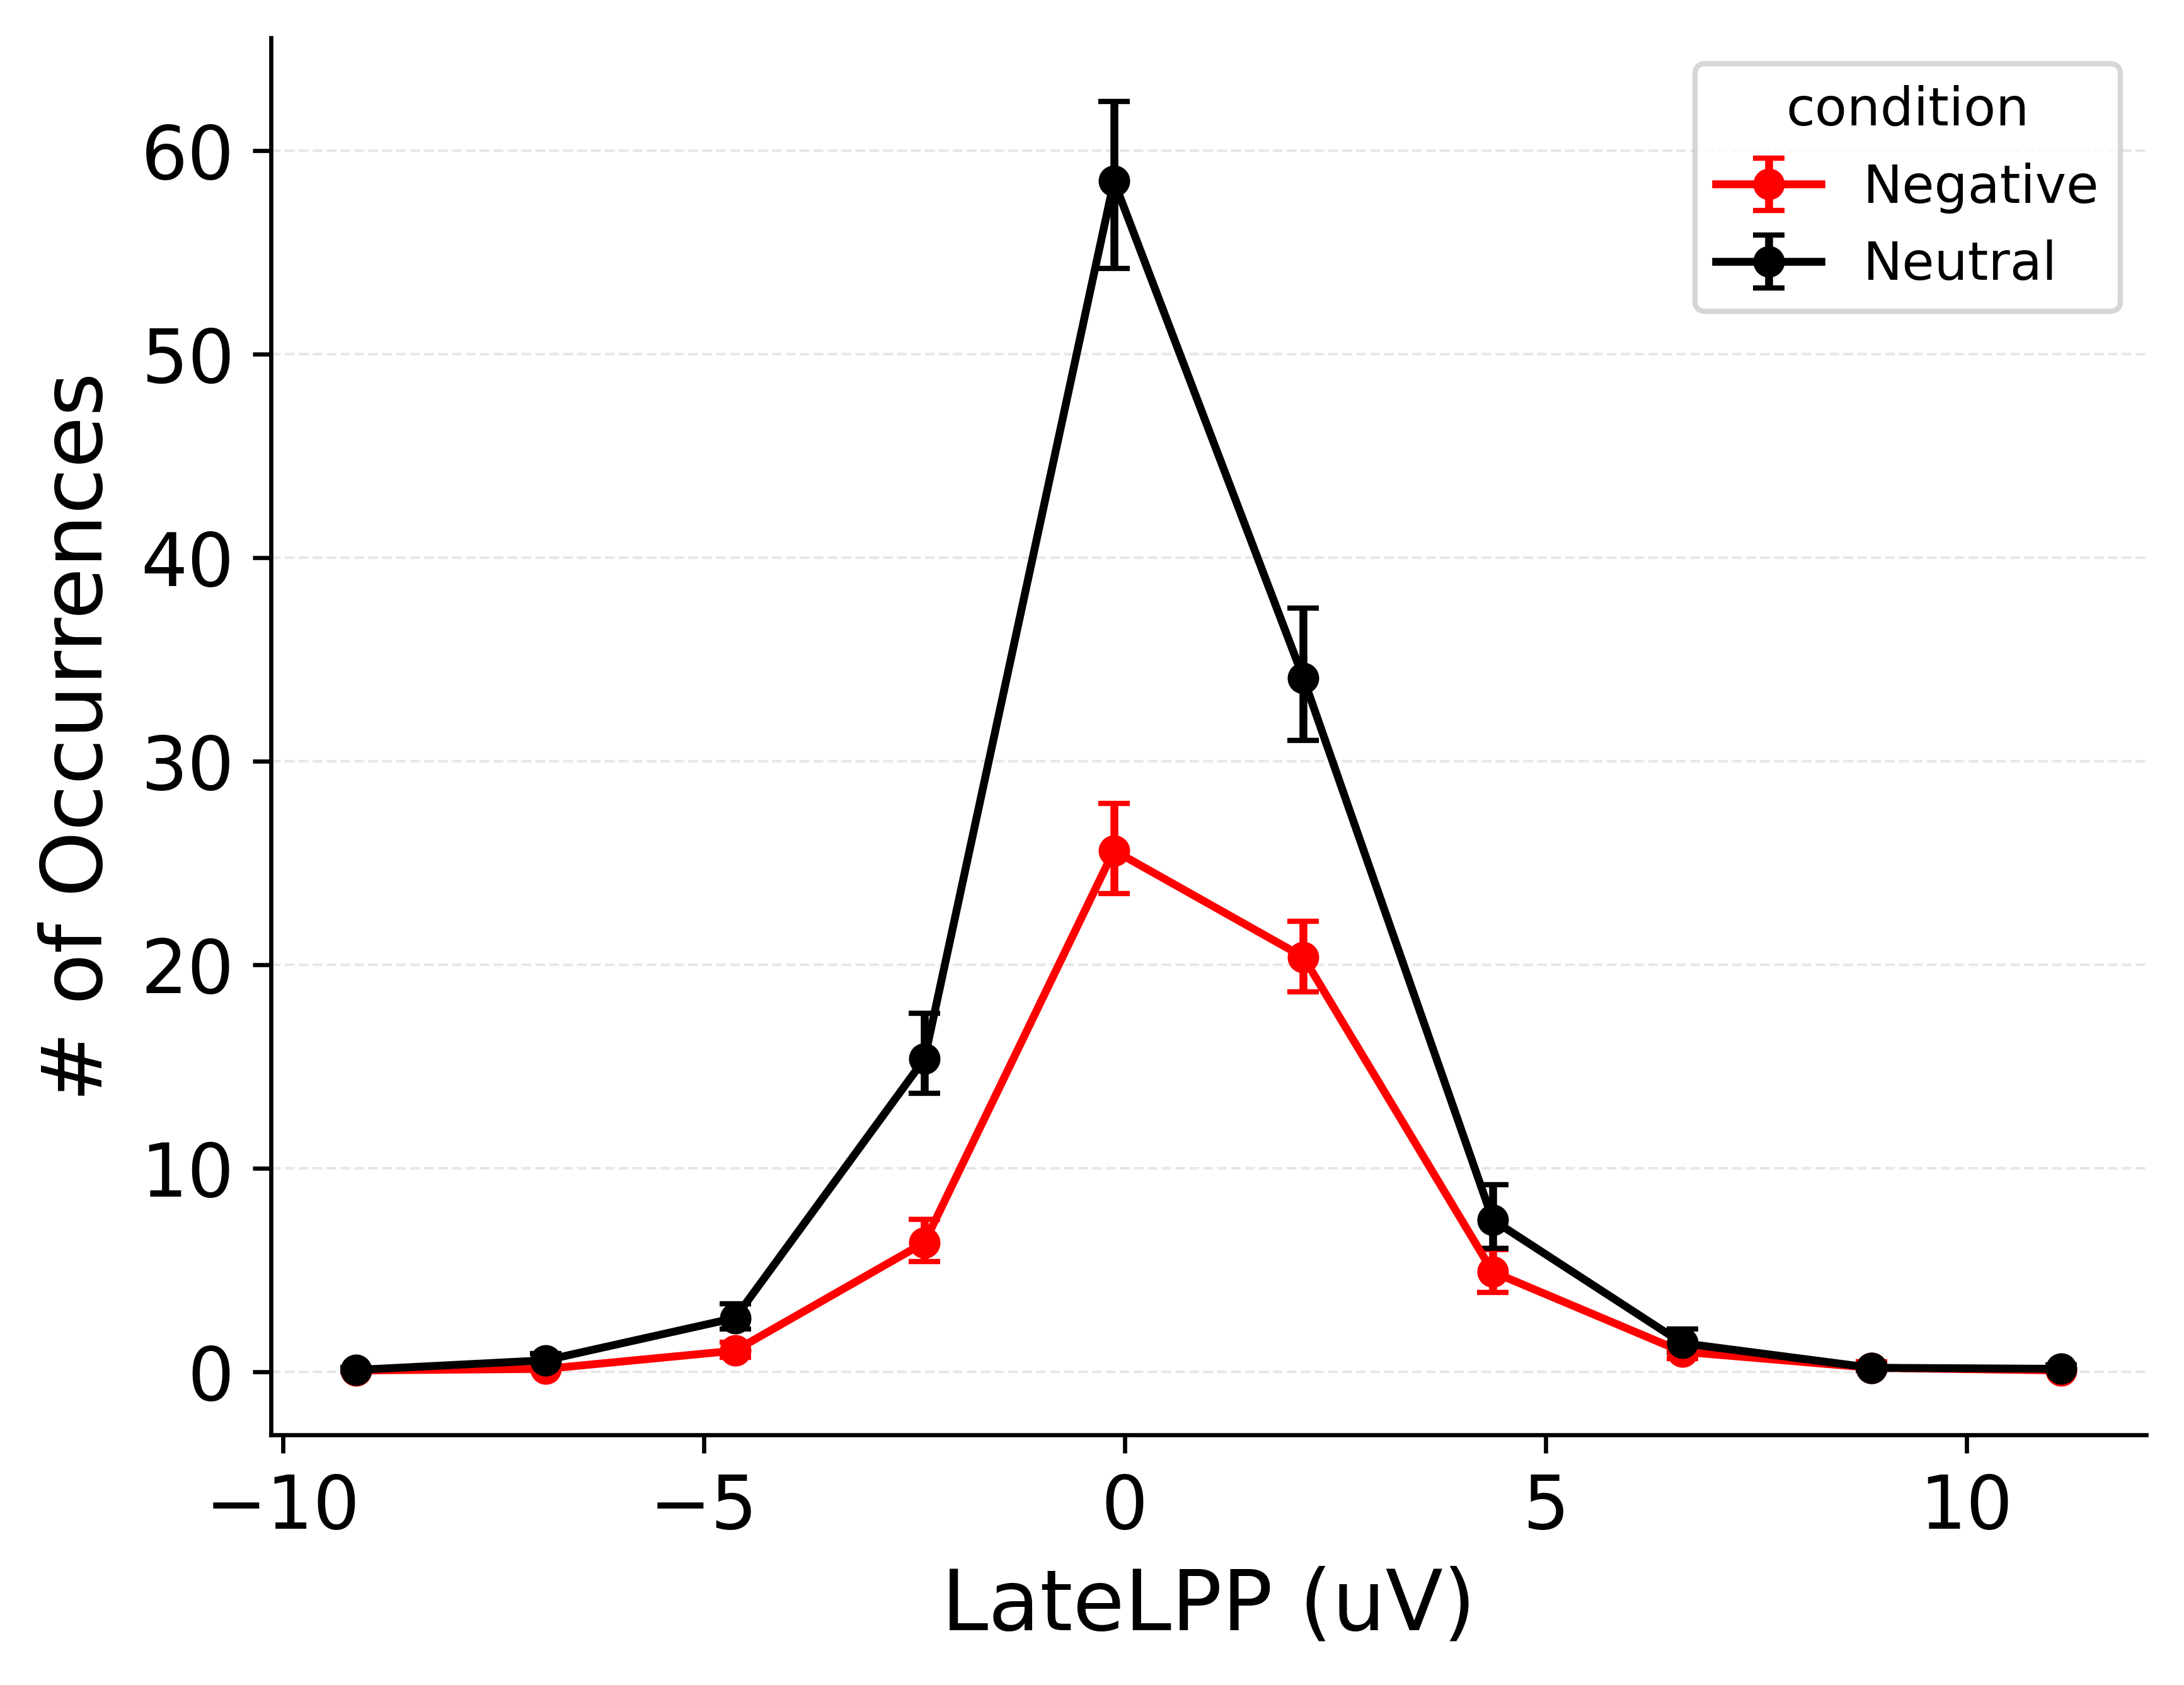
\includegraphics[keepaspectratio]{results/figures/analyses/cat_recall_by_lpp_LateLPP_counts.png}}\end{minipage}%

\end{figure}%

\subsection{Alternative Fitting Approaches
Considered}\label{alternative-fitting-approaches-considered}

\subsubsection{Simulation-Based Estimates of Set
Likelihood}\label{simulation-based-estimates-of-set-likelihood}

Before settling on the permutation-based set-likelihood procedure
described in the main text, we explored a more direct Monte Carlo
approach based on model-generated recall sequences. For each subject and
trial, we simulated many recall sequences from the model and then asked
how many of those simulations produced exactly the same recalled set as
observed in the data. The proportion of matching simulations provides an
unbiased Monte Carlo estimate of the set likelihood for that trial under
a given parameter setting.

In principle, this approach aligns closely with the generative structure
of the model: it directly samples from the joint distribution over
recall sequences induced by the encoding and retrieval dynamics. In
practice, however, it proved problematic. If no simulated sequence
happens to match the observed recalled set, the estimated likelihood for
that trial is zero, even when the parameter setting is reasonable. This
is particularly likely when many items are recalled on a list, because
the number of possible recall sequences that yield a given set grows
very quickly with set size. Even when some simulations do match the
observed set, the resulting likelihood estimates can be noisy unless a
large number of simulations are run per subject and trial, which makes
fitting costly and slow. These issues led us to favor the
permutation-based estimator used in the main analyses, which operates
over permutations of the observed set rather than over full simulated
sequences and thus avoids exact-match sparsity.

\subsubsection{Mean Squared Error Over Summary
Statistics}\label{mean-squared-error-over-summary-statistics}

We also experimented with a mean squared error (MSE) approach that fits
models to summary statistics rather than to trial-level recall sets. In
this scheme, we select one or more summary measures from the data (for
example, the Category-SPC), simulate the model under a candidate
parameter setting, compute the same statistics on the simulations, and
then score the fit by the mean squared difference between empirical and
simulated values. This approach is common in retrieved-context modeling
and is straightforward to implement and scale.

For the present dataset, fitting to the Category-SPC mainly tests
whether a model captures overall position effects and the average recall
advantage for emotional relative to neutral items. It is well suited to
assessing whether a neurally uninformed eCMR variant can reproduce the
emotional enhancement of memory (EEM), and indeed our neurally informed
extensions did not substantially improve fits to the Category-SPC
relative to their standard eCMR counterparts. This outcome is consistent
with what the mixed-effects analyses already suggest. The GMM results do
not imply that LPP should add much explanatory power for overall recall
rates of emotional versus neutral items beyond what is already captured
by the emotion labels themselves. Instead, they show that LPP is most
informative for distinguishing which \emph{emotional} items are more
likely to be recalled, with little additional predictive value for
neutral items.

Our neurally informed extensions were designed with this itemwise target
in mind. Parameters that act like a static emotional attention boost
(such as an ``emotion scale'' in standard eCMR or an LPP threshold used
to approximate an emotional boost) can capture EEM at the
serial-position-curve level. In contrast, parameters that link
trial-to-trial variations in LPP to variations in recall (such as an LPP
slope that modulates attention or binding strength) primarily influence
\emph{which} emotional items are recalled, not \emph{how many} emotional
items are recalled on average. As a result, MSE-based fits to summary
statistics like the Category-SPC are relatively insensitive to the
mechanisms we wish to test: they can confirm that emotional attention
mechanisms capture the EEM effect, but they are not well positioned to
detect improvements in explaining which items are recalled as a function
of LPP.

From this perspective, MSE over summary statistics is not ``less
rigorous'' than likelihood-based fitting, but it targets a different
question. It is most appropriate when the modeling goal is to match
coarse patterns such as overall recall rates and serial-position
effects. Our primary aim, however, is to evaluate neurally informed LPP
mechanisms that are intended to explain itemwise differences in recall
probability within the emotional condition. For that goal, a trial-level
set-likelihood objective, as described in the main text, provides a more
direct and sensitive test.

\subsection{Justification for Pure Main Effects
Model}\label{justification-for-pure-main-effects-model}

Consider a simplified ``spotlight'' view of retrieved-context dynamics.
At encoding, each item acquires an association strength or learning rate
\(S_i\). At retrieval, the activation of item \(i\) is roughly
proportional to a product of its trace strength and its match to the
current cue, for example

\[
A_i \propto (\text{cue–trace similarity}_i \times S_i)^\tau,
\]

followed by normalization across items. Importantly a sensitivity
parameter \(\tau > 1\) introduces nonlinear competition: items with
higher activation get disproportionately favored during recall. If
Emotion and LPP each contribute linearly to these ingredients (for
instance, adding to the learning rate and to the cue--trace match), then
the product contains an interaction term even when the encoding rule
itself includes only main effects. In other words, nonlinear
cue-dependent competition can generate an effective LPP × emotion
dependence in recall probabilities even without an explicit interaction
term in the learning-rate equation. This observation makes it a modeling
question, not a foregone conclusion, whether the interaction term
estimated by the GMM must be present at encoding or can arise as a
side-effect of retrieved-context dynamics. Together, these comparisons
address the core question without introducing additional structural
variants.

\section{Partial References}\label{partial-references}

\phantomsection\label{refs}
\begin{CSLReferences}{1}{0}
\bibitem[\citeproctext]{ref-friendly1982toronto}
Friendly, M., Franklin, P. E., Hoffman, D., \& Rubin, D. C. (1982). The
toronto word pool: Norms for imagery, concreteness, orthographic
variables, and grammatical usage for 1,080 words. \emph{Behavior
Research Methods \& Instrumentation}, \emph{14}(4), 375--399.

\bibitem[\citeproctext]{ref-healey2014memory}
Healey, M. K., \& Kahana, M. J. (2014). Is memory search governed by
universal principles or idiosyncratic strategies? \emph{Journal of
Experimental Psychology: General}, \emph{143}(2), 575.

\bibitem[\citeproctext]{ref-storn1997differential}
Storn, R., \& Price, K. (1997). Differential evolution--a simple and
efficient heuristic for global optimization over continuous spaces.
\emph{Journal of Global Optimization}, \emph{11}(4), 341--359.

\end{CSLReferences}






\end{document}